\chapter{Experiments} \label{chap-5}

This chapter presents the results of initial experimental studies of the production of an approximate Danilov distribution in the SNS ring by means of the elliptical painting method. The simulations in chapters \ref{chap-2}-\ref{chap-3} were used to guide the experiments, and the diagnostics described in Chapter \ref{chap-4} were used to measure the painted distribution.

Recall the definition of elliptical painting: the injected beam coordinates are scaled along an eigenvector of the one-turn transfer matrix. Each eigenvector, $\mathbf{v}_1$ or $\mathbf{v}_2$, traces an ellipse in the $x$-$y$ plane on a turn-by-turn basis, so elliptical painting can be performed in any ring. Yet a number of factors determine whether the painted distribution resembles a Danilov distribution. Consider the following three scenarios:

\begin{table}[h!]
    \centering
    \begin{tabularx}{1.0\textwidth} { 
        | >{\raggedright\arraybackslash}X 
        | >{\raggedright\arraybackslash}X | }
     \hline
     \textbf{Scenario} & \textbf{Turn-by-turn eigenvector behavior in $x$-$y$ plane} \\
     \hline
     (1) Uncoupled optics; unequal tunes & $\mathbf{v}_1$ traces a horizontal line and $\mathbf{v}_2$ traces a vertical line. \\
     \hline
     (2) Uncoupled optics; equal tunes & Same as (1), but any linear combination of $\mathbf{v}_1$ and $\mathbf{v}_2$ is an eigenvector and traces an ellipse. \\
     \hline
     (3) Coupled optics & It is possible for each eigenvector to trace an ellipse. \\
    \hline
    \end{tabularx}
    \label{tab:painting_scenarios}
\end{table}

Elliptical painting would produce a flat beam in Scenario (1) but a round beam in Scenarios (2) and (3). Scenario (3) is preferred because simulations indicate that it is more stable against imperfections than Scenario (2). Recall from Chapter \ref{chap-3} that the effect of solenoid magnets in the SNS ring has already been studied. Solenoid magnets were planned to be installed in the SNS ring in 2021, but their installation was delayed until late 2022, outside the time frame of this work; therefore, in the following experiments, the elliptical painting method was carried out by setting equal tunes in the ring (Scenario (2)). Although the quality of the final beam was not expected to approach the ``best-case scenario" simulated in Chapter \ref{chap-3}, it was hoped that it would be clearly distinguishable from a beam produced by traditional methods. 

A brief outline of this chapter: First, the experimental setup and data collection procedure is described. In Experiment 1, a production beam was measured for comparison and elliptical painting was attempted, but unsuccessful, at a beam energy of 1 GeV. In Experiment 2, the beam energy was lowered to 0.8 GeV to allow proper scaling of the injected beam coordinates. In Experiment 3, several parameters were varied to study the effect on the 4D emittance of the painted beam. Finally, the implications of these measurements are discussed.


\section{Procedure}

Accelerator physics experiments are performed in the SNS control room using the OpenXAL framework, which provides a high-level interface to perform tasks such as changing magnet strengths, triggering the beam, etc. It can also perform single-particle or envelope tracking using an online model of the accelerator. OpenXAL scripts are written in Java or Jython and are executed from the command line. Many graphical user interface (GUI) OpenXAL applications have been developed over the history of the SNS and are available for use in the control room. 

The following steps are taken during the experimental setup:
%
\begin{enumerate}
    \item 
    To reach the closed orbit to the foil, the beam energy is lowered from 1.0 GeV to 0.8 GeV by turning off several RF cavities at the end of the linac. This is performed by the SNS operations team. Generally, lowering the energy causes other accelerator components to trip or malfunction due to the modified timing system, and these must be corrected one-by-one. The first attempt to lower the energy to 0.8 GeV took over six hours.
    %
    \item
    The horizontal and vertical tunes are set to the same value using the Ring Optics Control (ROC) application. ROC varies several quadrupoles until the model tunes are equal to the desired tunes. The tunes are measured using turn-by-turn BPM readings from a single minipulse in the ring. Generally, the measured and model tunes are not quite equal; we therefore shift the ROC input tunes until the measured tunes converge to the desired tunes. 
    %
    \item
    Optional: The injection region is modified in some way to assist the injection kickers.
    %
    \item
    The eight injection kicker magnets are calibrated using the Ring Injection Control (RIC) application, as described in Chapter \ref{chap-1}. 
    %
    \item
    The initial/final kicker voltages are determined to obtain the desired closed-orbit coordinates at the foil, as described in Chapter \ref{chap-1}.
    %
    \item
    The initial/final voltages are connected with a square root waveform, and the waveform is applied to the injection kickers. The painting time (the duration of the waveform) is chosen at this step but can be changed later on. The painting time determines the number of minipulses in the final distribution, i.e., the beam intensity.
    %
    \item
    The number of injected turns before extraction is chosen. This allows the distribution to be measured at different times during injection. It is also possible to store the beam in the ring, although the SNS normally extracts the beam immediately after accumulation.
    %
\end{enumerate}
%
The next task is to prepare for the measurements. For the wire-scanner measurement, the first step is to modify the RTBT optics using the application developed in Chapter \ref{chap-4}. If the fixed-optics method is used, the optics are changed immediately. If the multi-optics method is used, the optics are pre-computed and stored for later use. 

The second possible measurement is the tomographic reconstruction from $x$-$y$ projections on the target. Since the optics calculation is time-consuming, it can be run in the background while wire-scans are collected. The use of target images for tomographic reconstruction was proposed late in this research, so the target scan was only performed in the last of the following experiments.


\section{Experiment 1}

The SNS reserves approximately two days per month for accelerator physics experiments, and various experiments must compete for time within this forty-eight hour period. At the time of our first experiment, setup of the injection region using the RIC application had not yet been completed. Although simulations indicated that the kickers were not strong enough to perform elliptical painting at 1 GeV kinetic energy, this had not been tested. And the SNS energy had not yet been decreased — a time-consuming and possibly error-prone task. The goal of Experiment 1 was therefore to push the injected coordinates $x$ and $y'$ to their limits at 1 GeV.

We decided to measure the distribution not only at its final state, but also at the intermediate states. Using the fixed-optics method, ten measurements could be performed within one hour. 

\subsection{Experiment 1a: correlated painting}

We first performed correlated painting for comparison. Recall that in correlated painting the displacements at the foil are increased from an initial offset to their final value, and the slope at the foil is always zero. The number of injected turns was reduced from 1000 to 500, and the beam was measured every 50 turns. 

The measured wire-scanner profiles are shown in Fig.~\ref{fig:exp1a_wsmeas}.
%
\begin{figure}[!p]
    \centering
    \begin{subfigure}{\textwidth}
        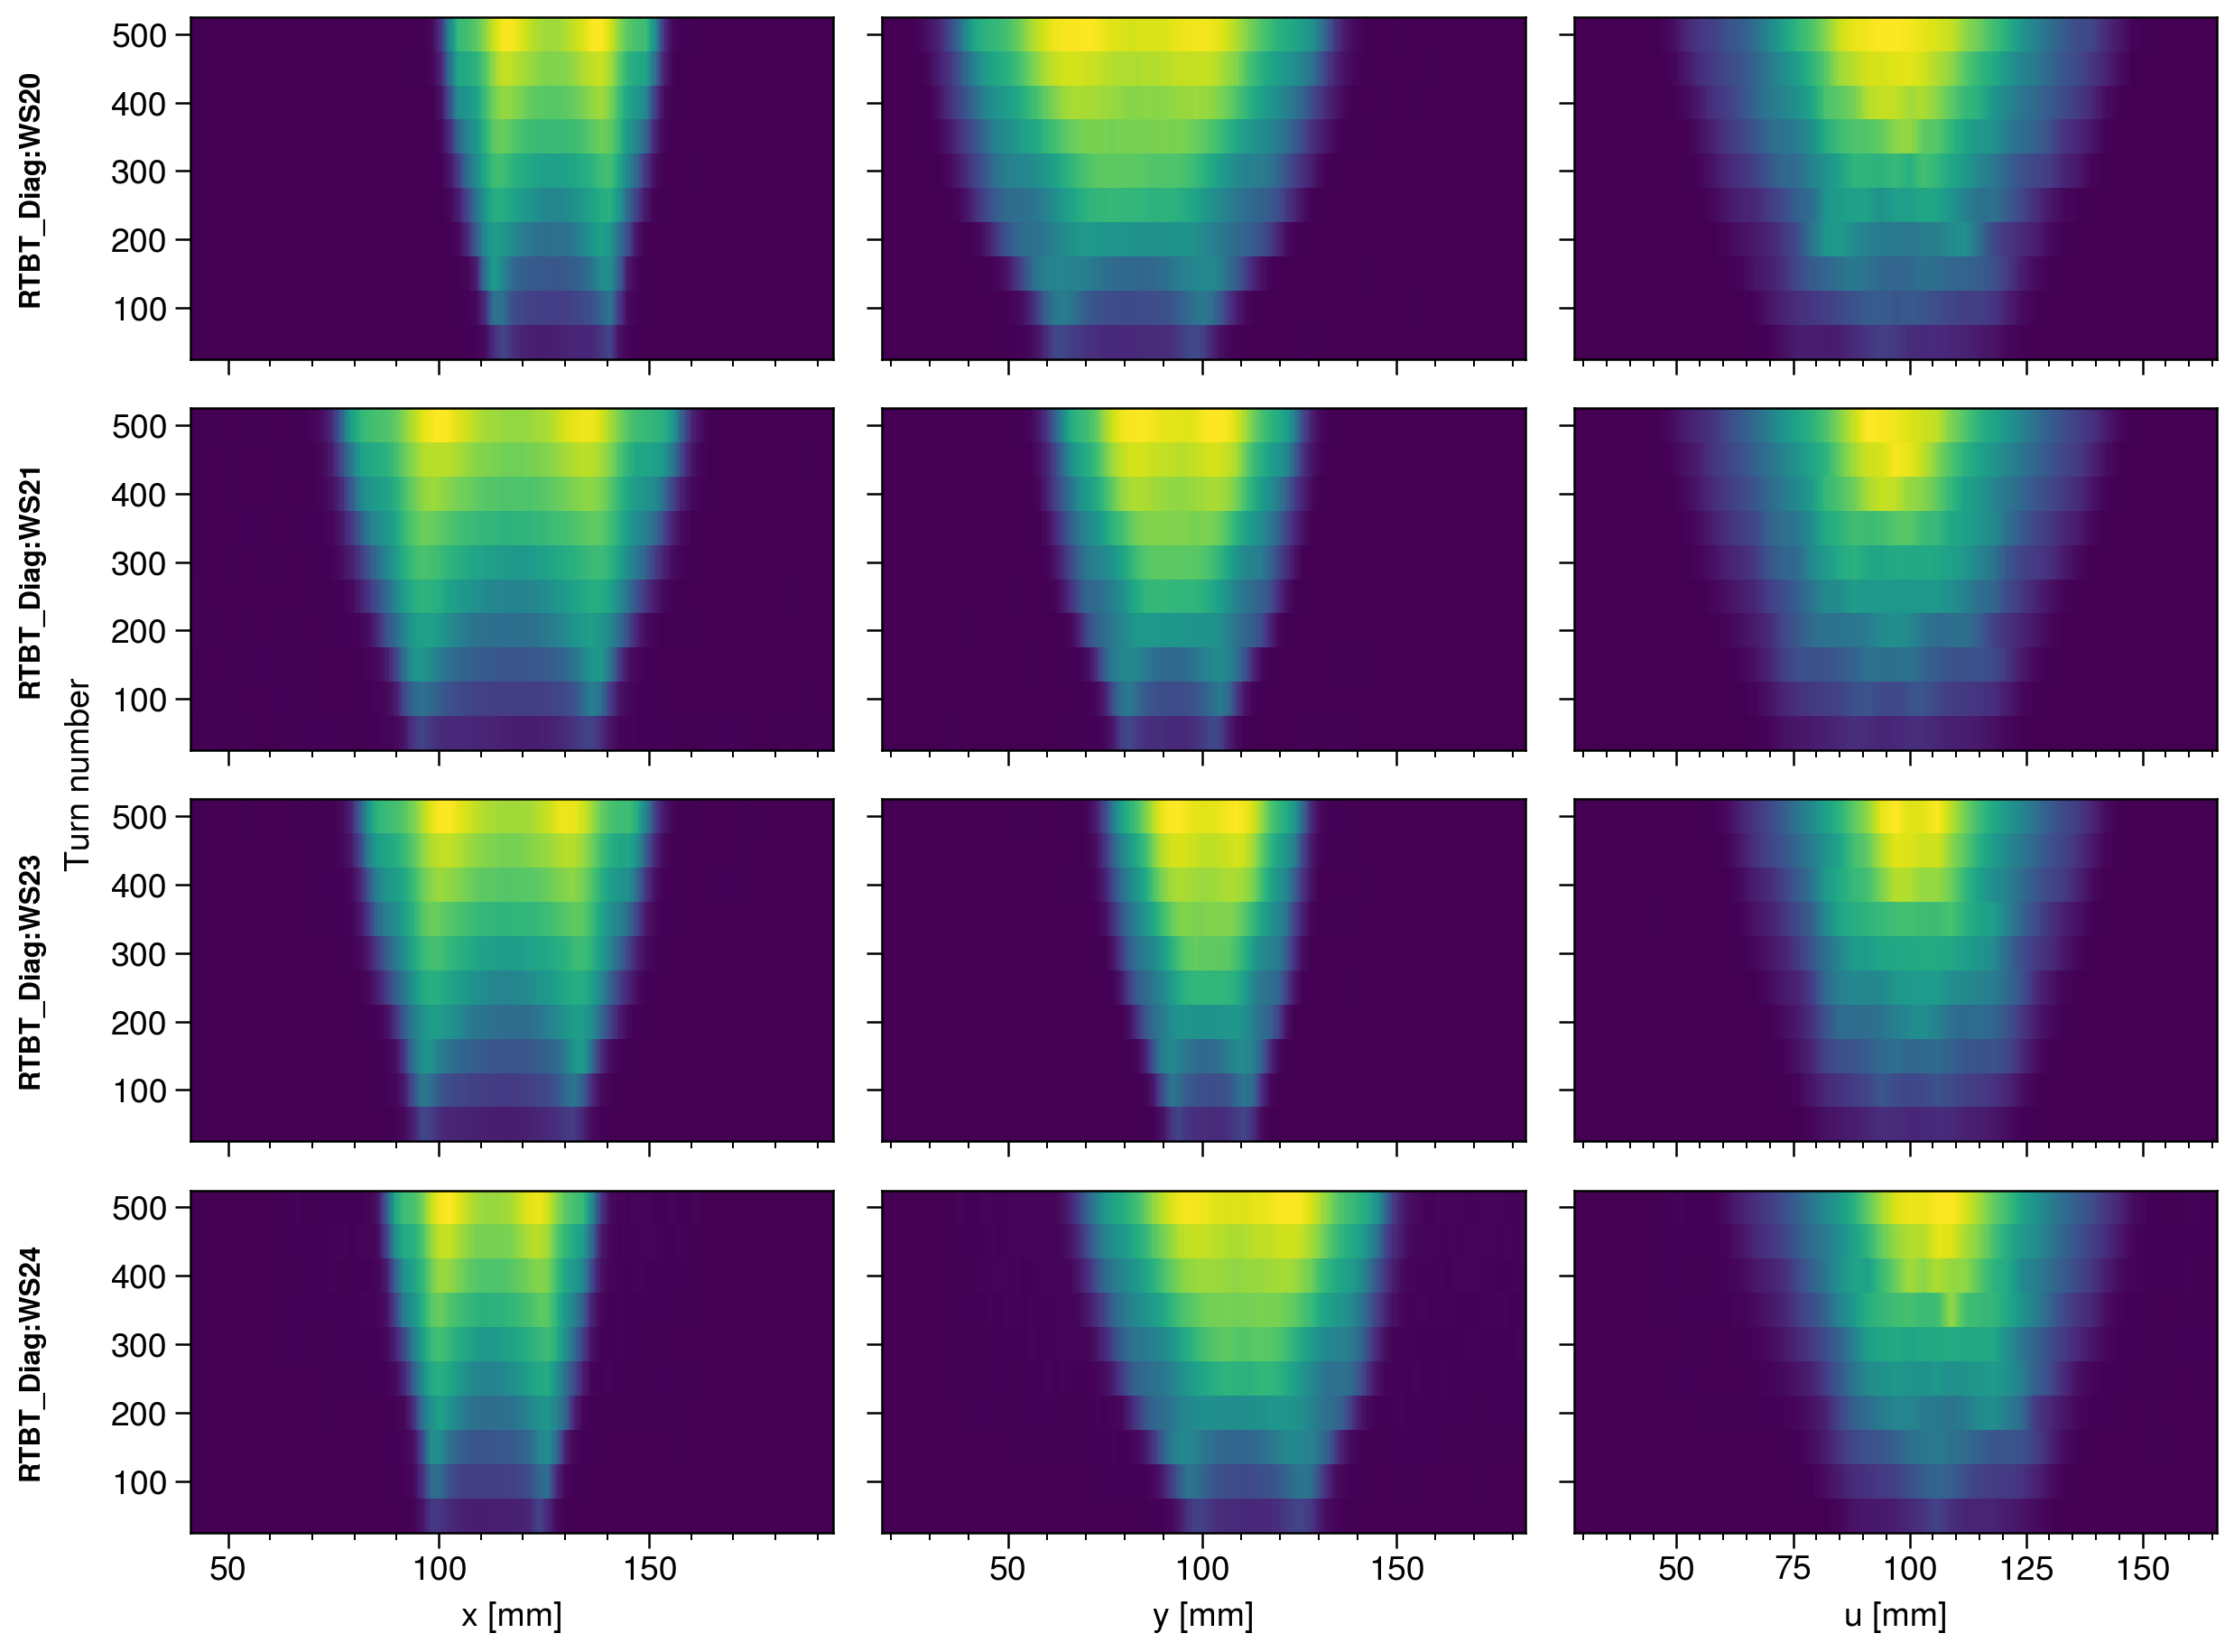
\includegraphics[width=\textwidth]{Images/chapter5/exp1a/waterfall.png}
    \end{subfigure}
    \vfill
    \vspace*{1.25cm}
    \vfill
    \begin{subfigure}{\textwidth}
        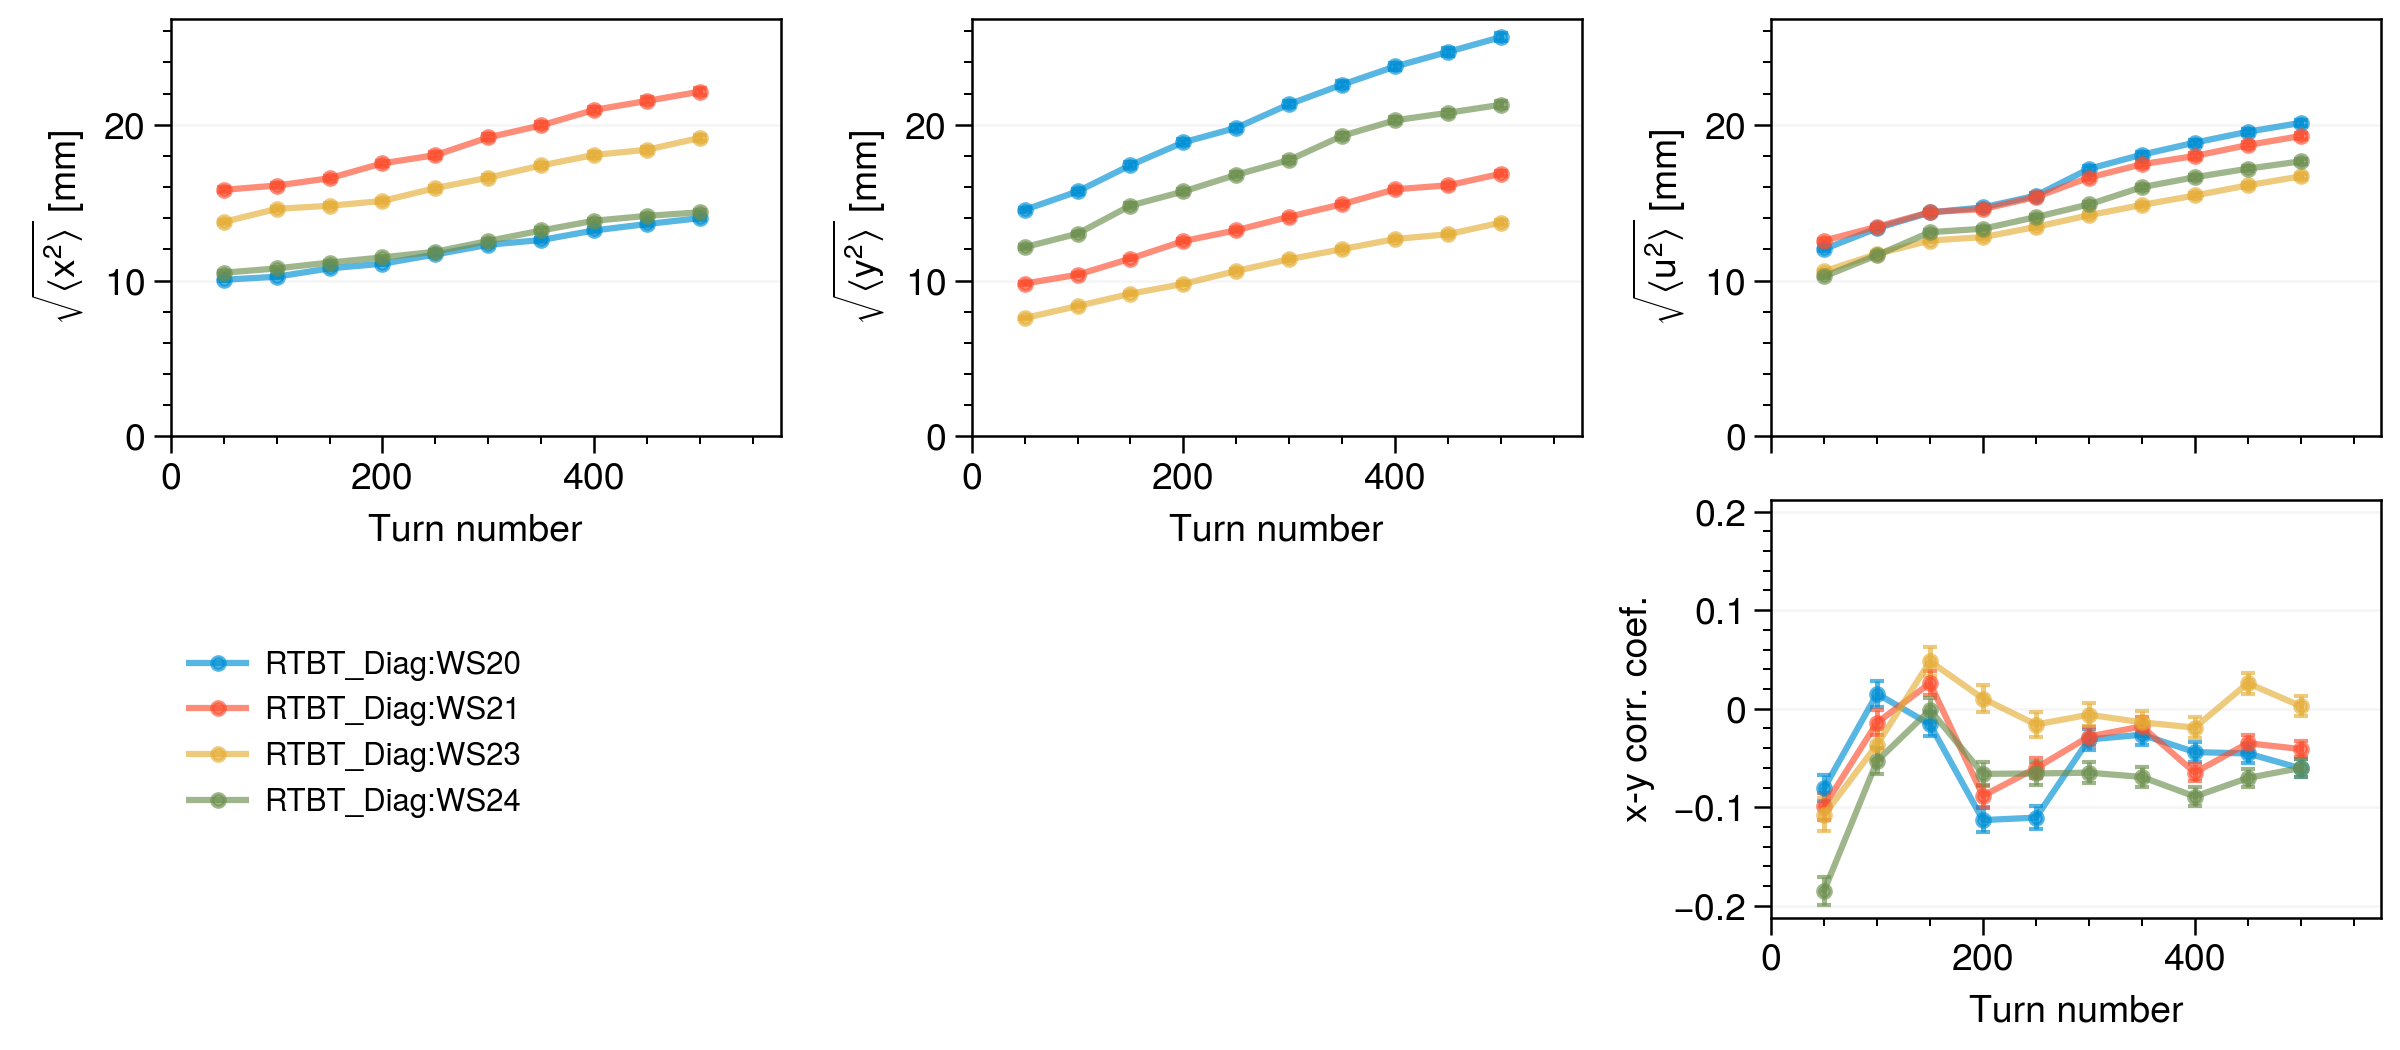
\includegraphics[width=\textwidth]{Images/chapter5/exp1a/rms.png}
    \end{subfigure}
    \caption{Measured wire-scanner profiles from Experiment 1a.}
    \label{fig:exp1a_wsmeas}
\end{figure}
%
%
\begin{figure}[!p]
    \centering
    \begin{subfigure}{0.6\textwidth}
        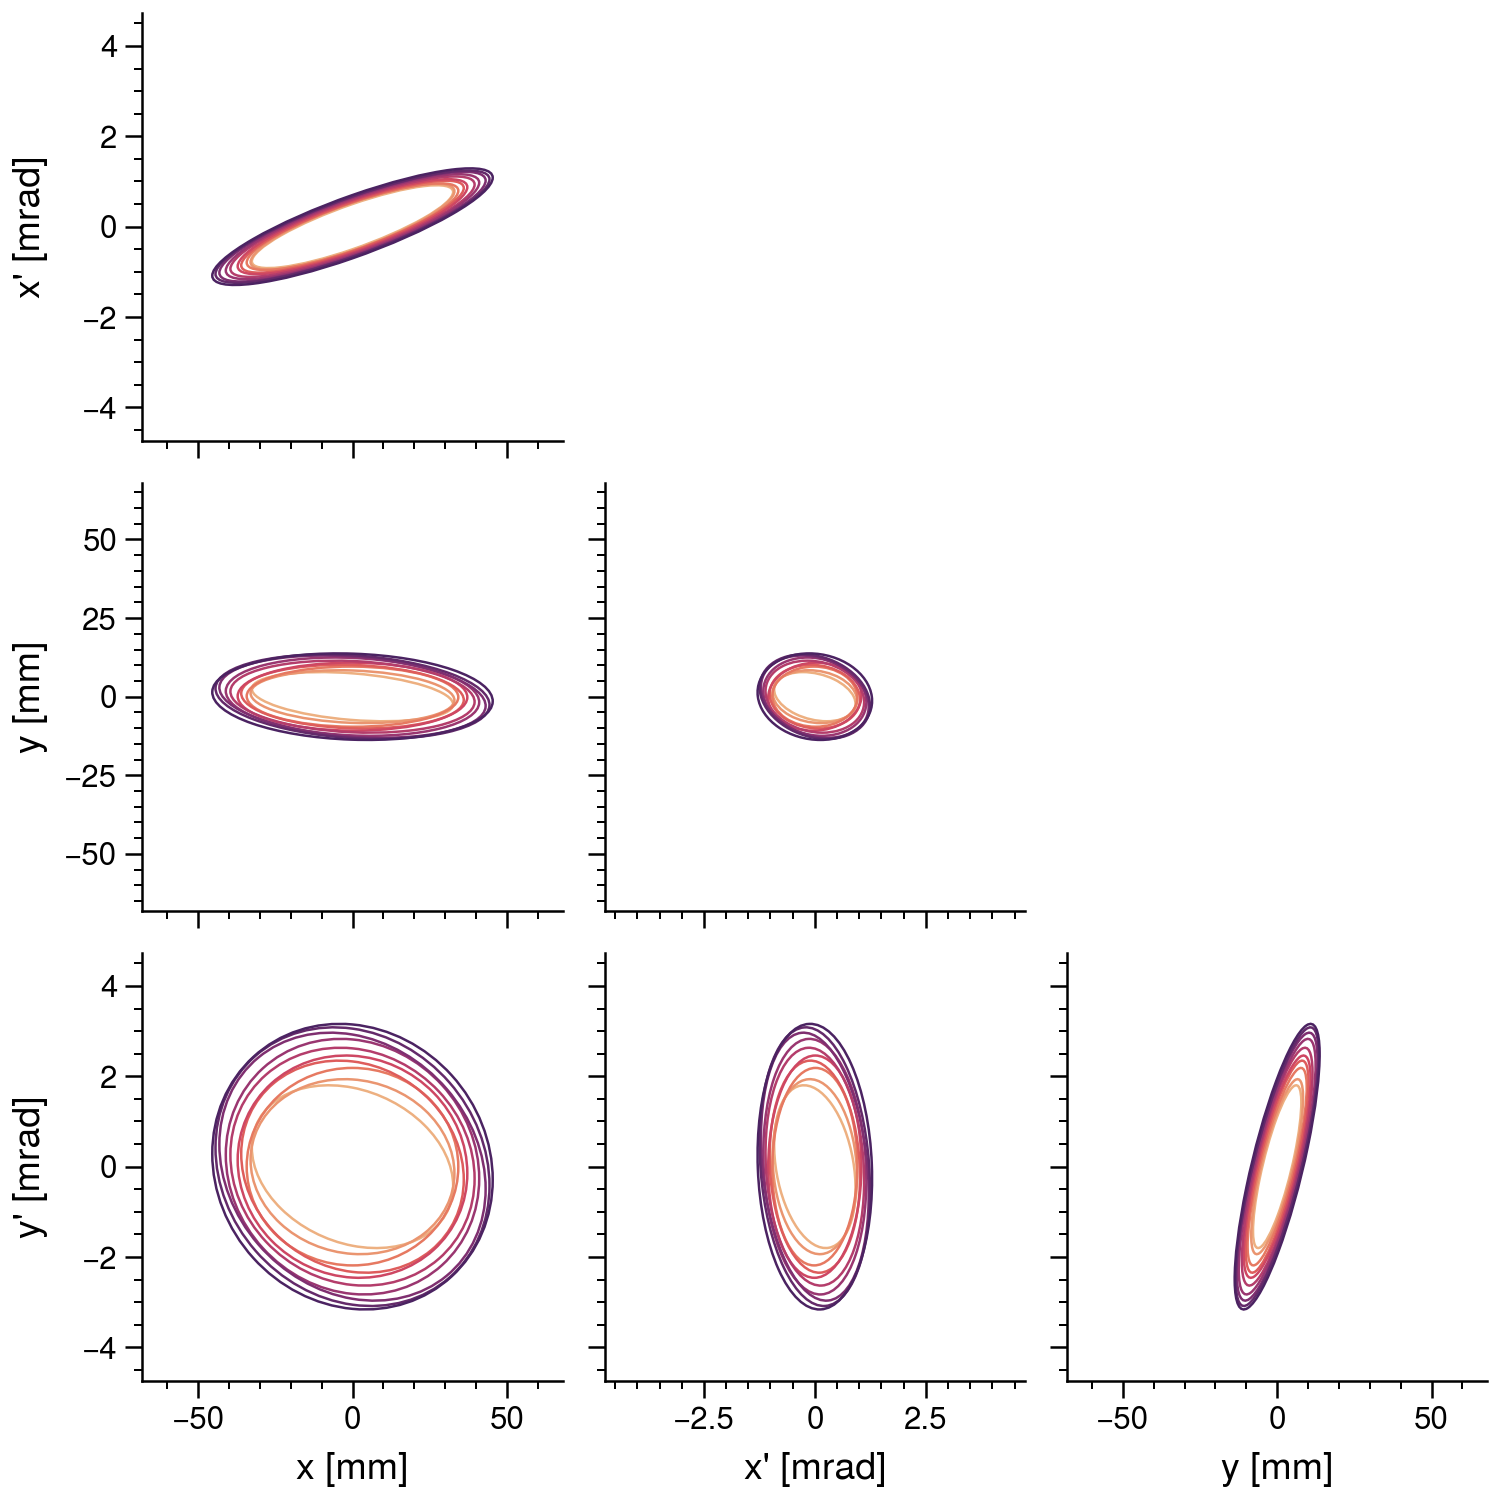
\includegraphics[width=\textwidth]{Images/chapter5/exp1a/corner.png}
    \end{subfigure}
    \hfill
    \begin{subfigure}[t]{0.39\textwidth}
        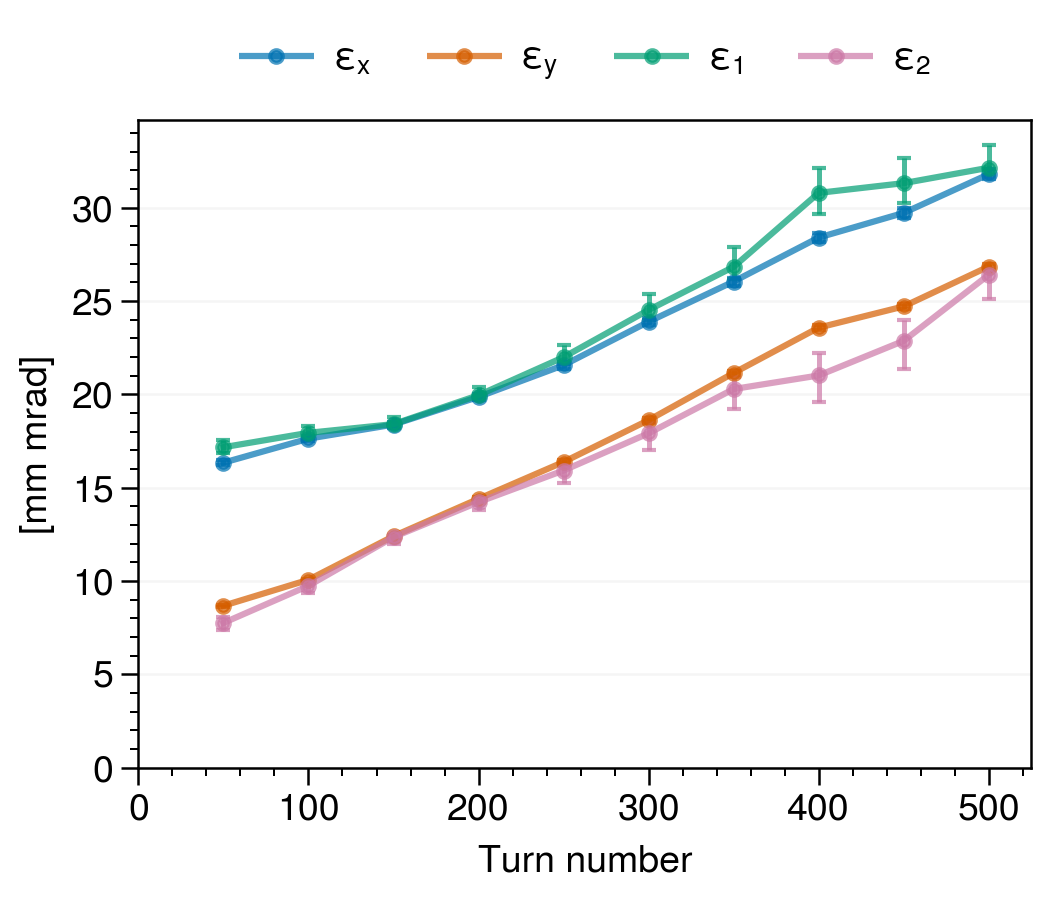
\includegraphics[width=\textwidth]{Images/chapter5/exp1a/emittances.png}
    \end{subfigure}
    \caption{Reconstructed emittances and covariance ellipses from Experiment 1a. In this and subsequent figures, the reconstruction is performed at BPM17 and the light/dark ellipses correspond to the start/end of injection.}
    \label{fig:exp1a_emittances}
\end{figure}
%
Each subplot shows the evolution of the projection onto a single wire; each row corresponds to a different wire-scanner and each column corresponds to a different projection axis — $x$, $y$, or $u$. That the closed orbit starts offset from the foil is evident from two initial peaks in the $x$ and $y$ projections. The distribution likely starts as a donut in $x$-$x'$ and $y$-$y'$, the hollow centers of which eventually partially fill in due to space charge and other nonlinear effects.

The reconstructed emittances and covariance ellipses at BPM17, just before QH18, are shown in Fig.~\ref{fig:exp1a_emittances}. Notice that the $x$-$x'$ and $y$-$y'$ ellipses maintain their shape and orientation over time while growing in area, which shows that the beam is matched to the ring optics in those planes. For our purposes, the main feature of Fig.~\ref{fig:exp1a_emittances} is that the measured cross-plane correlation is small, as expected. The error bars are calculated by repeating the reconstruction many times with noise added to the measured moments, then taking the mean and standard deviation over the trials. This can lead to asymmetric error bars. Previous measurements indicate that the moments estimated from the profiles have less than 2\% variation if the measurement is repeated, so we sampled within $\pm$ 2\% of the measured moments.

It is also possible to reconstruct the covariance matrix at different locations. Fig.~\ref{fig:exp1a_rec_betas_throughout} shows the reconstructed $\beta$ functions throughout the RTBT.
%
\begin{figure}[!p]
    \centering
    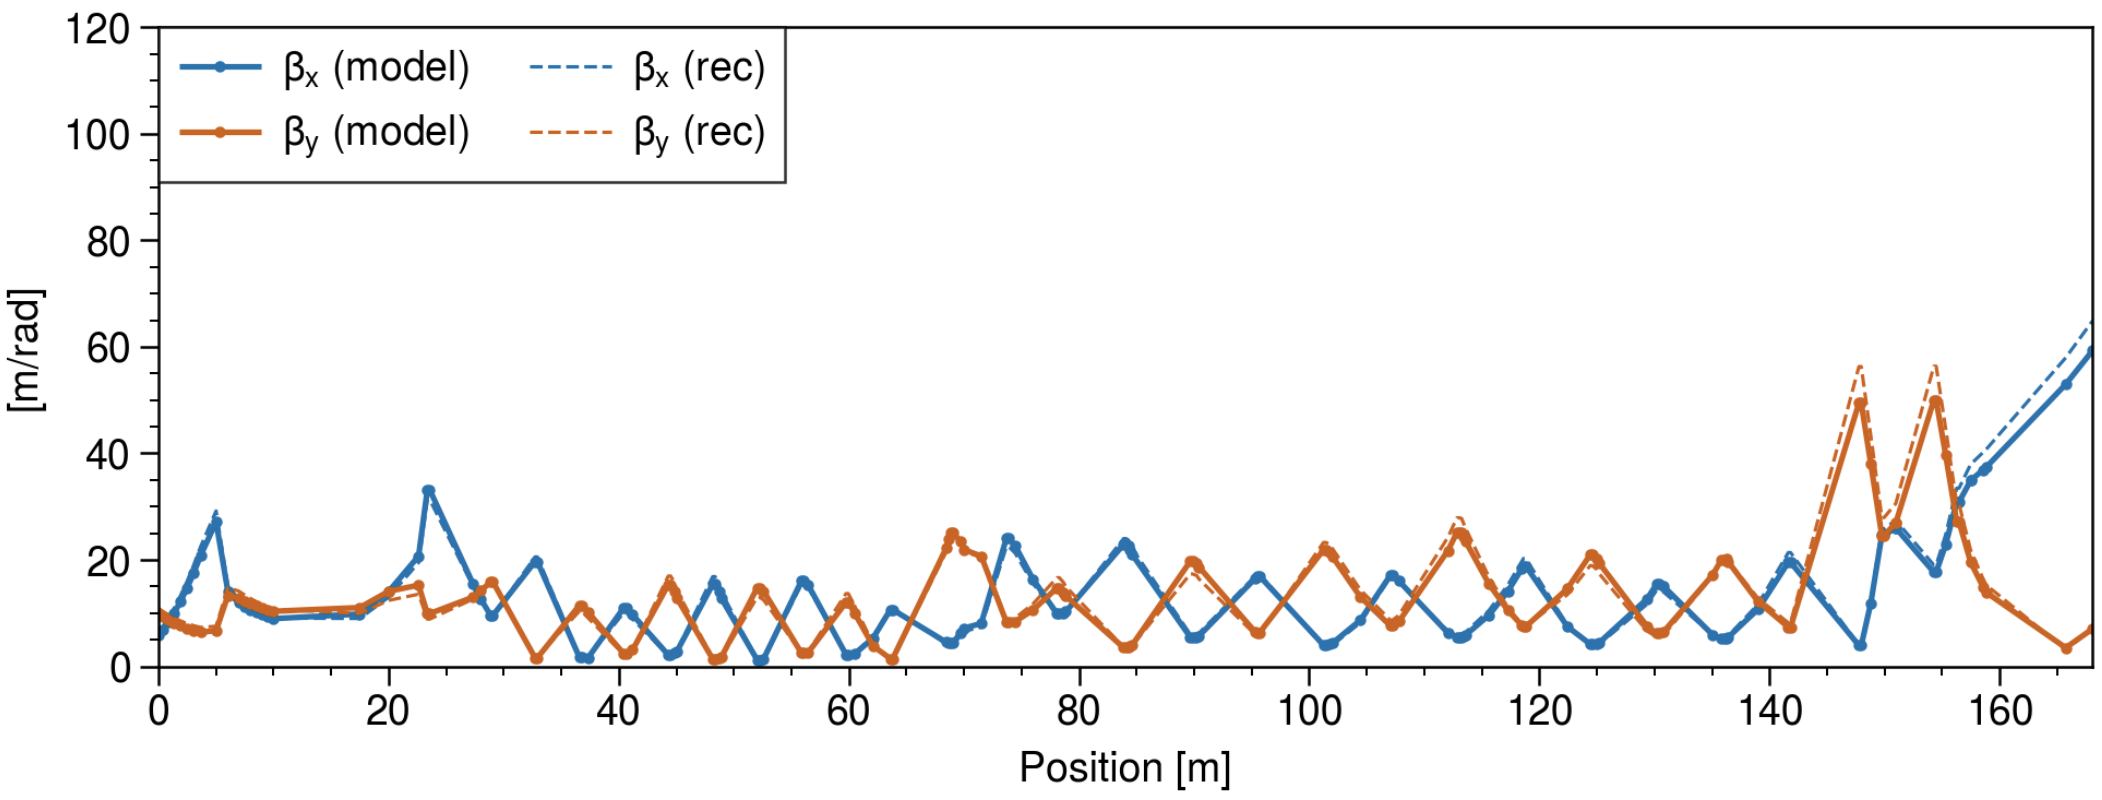
\includegraphics[width=1.0\textwidth]{Images/chapter5/exp1a/rec_betas_throughout.png}
    \caption{Reconstructed $\beta$ functions from Experiment 1a.}
    \label{fig:exp1a_rec_betas_throughout}
\end{figure}
%
The model parameters are computed from the linear transfer matrix of the ring + RTBT. This figure raises our confidence that the within-plane emittance measurements are accurate, and again shows that the beam is matched to the ring optics.



\subsection{Experiment 1b: attempted elliptical painting}

Next, we attempted to carry out elliptical painting. First, the horizontal and vertical tunes were set to 6.18. The next step was to move the closed orbit to the foil, which was found to be possible in the vertical plane but impossible in the horizontal plane; the minimum distance from the foil was 10 mm. Additionally, the maximum possible vertical slope was 0.7 mrad. It was decided to continue with the painting method using initial coordinates ($x$, $x'$, $y$, $y'$) $\approx$ (10 mm, 0 mrad, 0 mm, 0 mrad) and final coordinates ($x$, $x'$, $y$, $y'$) $\approx$ (21 mm, 0 mrad, 0 mm, 0.7 mrad). Using these settings, the initial beam would be a donut in $x$-$x'$ and a point in $y$-$y'$. In real space, it would be a flat horizontal line with higher density on the two ends of the line. In other words, injected particles would move along an ellipse in the $x$-$y$ plane with zero vertical size. As time progressed, the horizontal and vertical size of the ellipse would grow at different rates depending on the maximum painting $x$ and $y'$ coordinates. This is all assuming linear transport and non-interacting particles. Without a computer, it is unclear what would happen with the inclusion of space charge.

The measured wire-scanner profiles are shown in Fig.~\ref{fig:exp1b_wsmeas}, and the reconstructed emittances and covariance ellipses at BPM17 are shown in Fig.~\ref{fig:exp1a_emittances}.
%
\begin{figure}[!p]
    \centering
    \begin{subfigure}{\textwidth}
        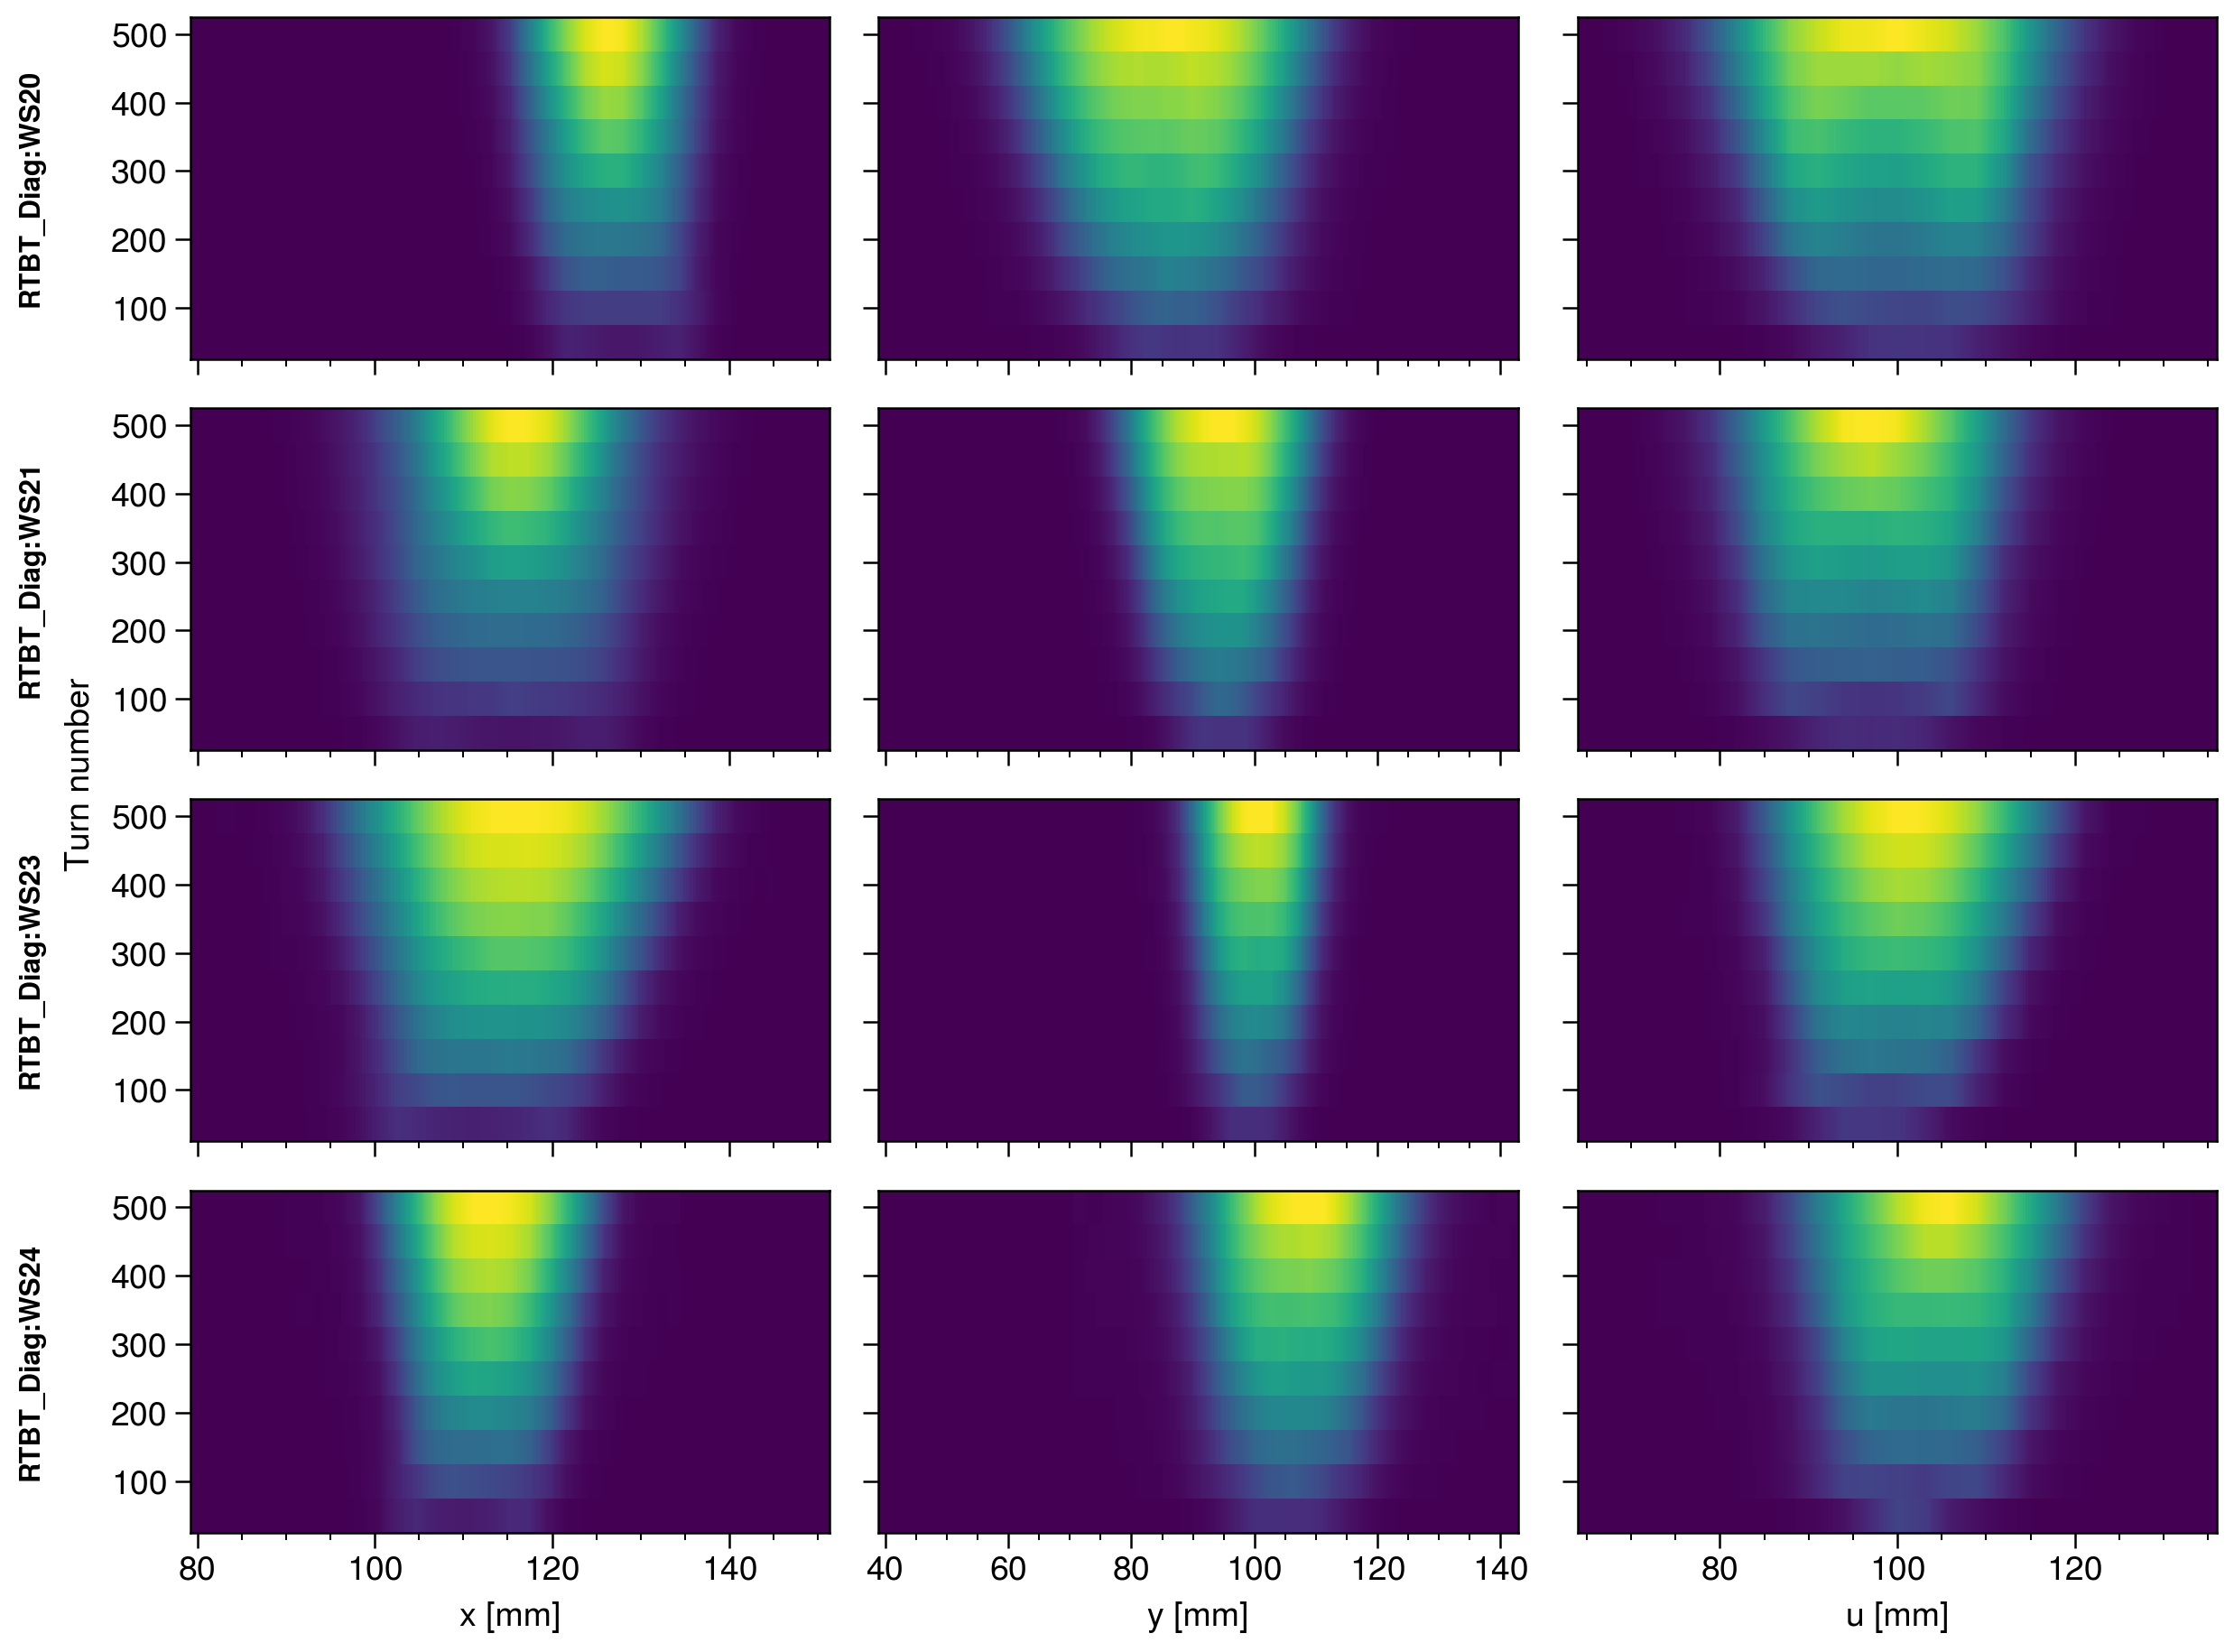
\includegraphics[width=\textwidth]{Images/chapter5/exp1b/waterfall.png}
    \end{subfigure}
    \vfill
    \vspace*{1.25cm}
    \vfill
    \begin{subfigure}{\textwidth}
        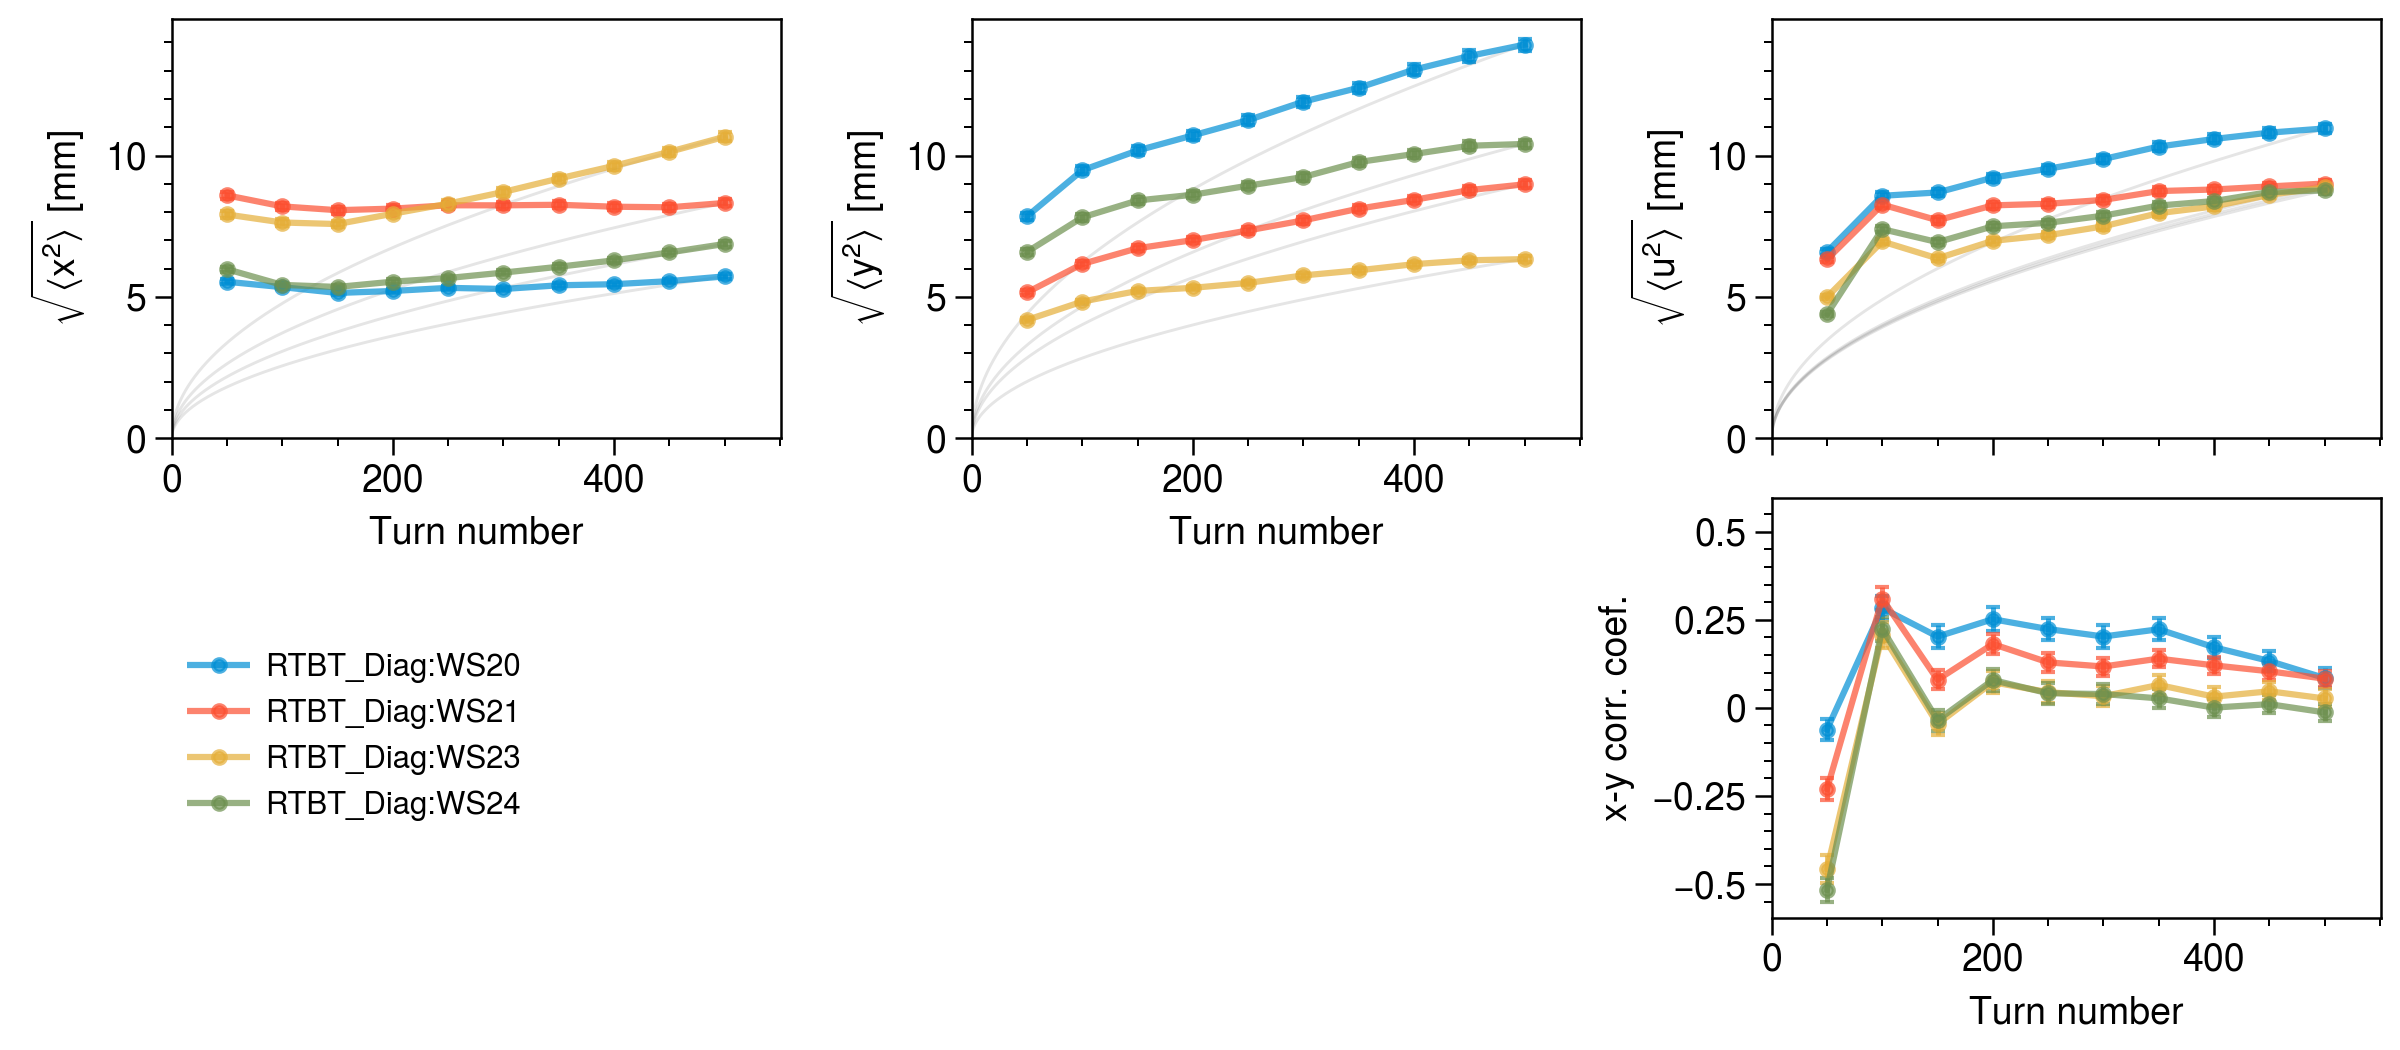
\includegraphics[width=\textwidth]{Images/chapter5/exp1b/rms.png}
    \end{subfigure}
    \caption{Measured wire-scanner profiles from Experiment 1b.}
    \label{fig:exp1b_wsmeas}
\end{figure}
%
%
\begin{figure}[!p]
    \centering
    \begin{subfigure}{0.6\textwidth}
        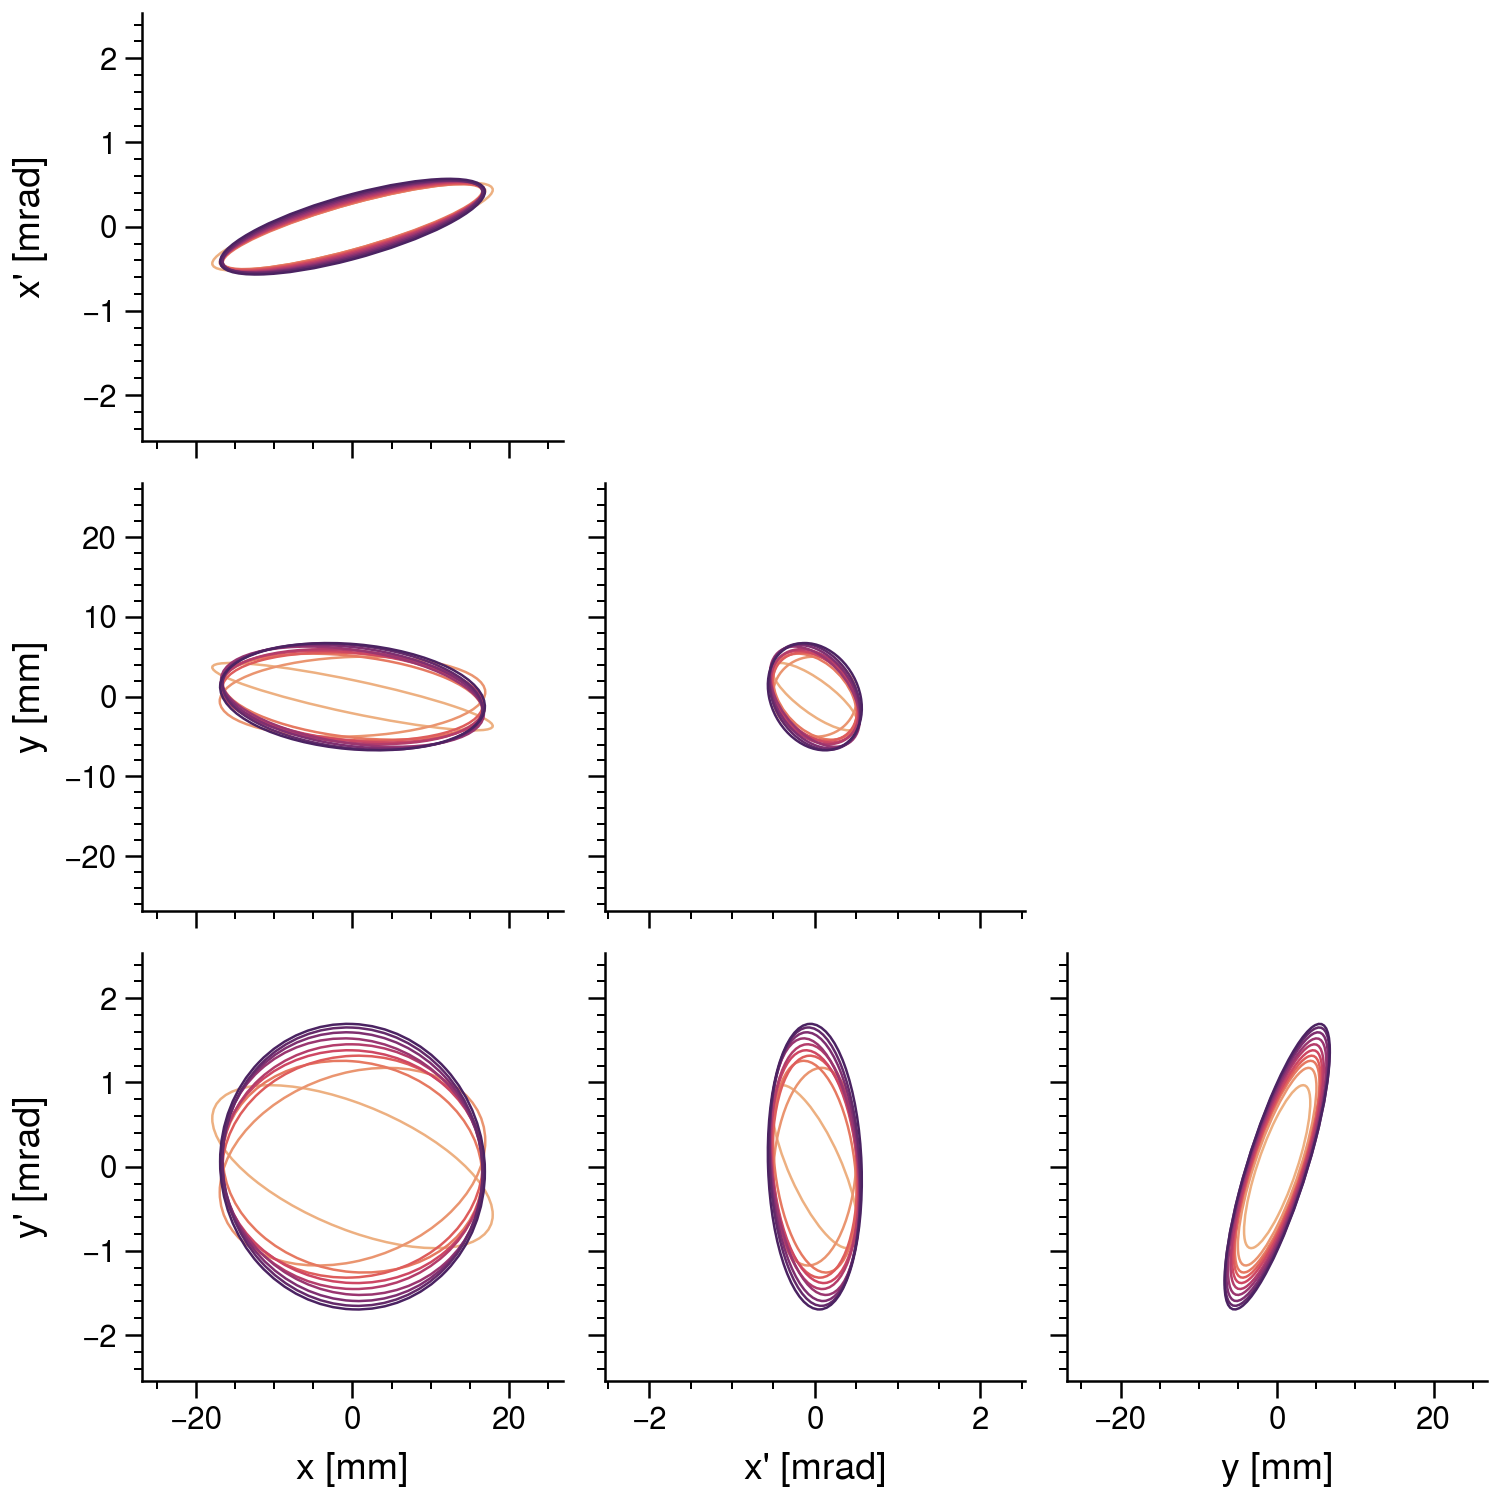
\includegraphics[width=\textwidth]{Images/chapter5/exp1b/corner.png}
    \end{subfigure}
    \hfill
    \begin{subfigure}[t]{0.39\textwidth}
        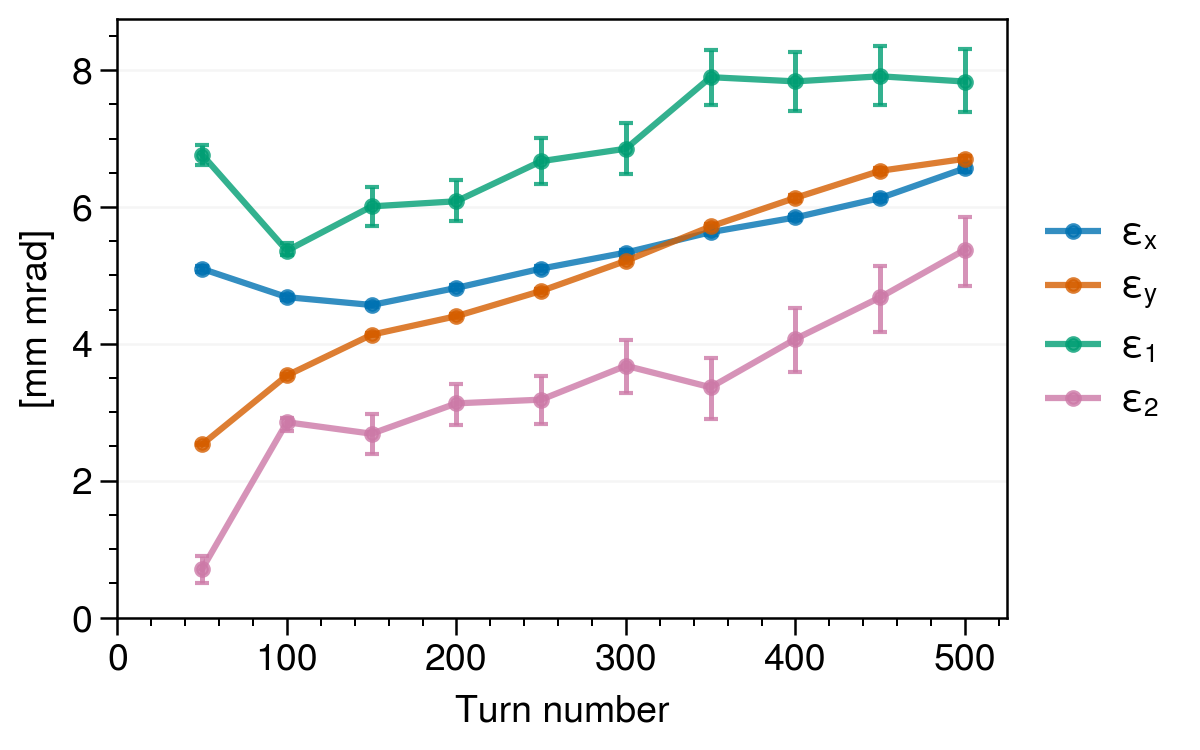
\includegraphics[width=\textwidth]{Images/chapter5/exp1b/emittances.png}
    \end{subfigure}
    \caption{Reconstructed emittances and covariance ellipses from Experiment 1b.}
    \label{fig:exp1b_emittances}
\end{figure}
%
Notice the growth of the vertical beam size in comparison with the horizontal size. The $x$-$x'$ distribution likely began as a donut and filled in over time while also growing in radius, hence the relative lack of growth in the horizontal beam size. The vertical beam size, on the other hand, starts at a small value and increases throughout injection. Additionally, there is now a clear separation between the intrinsic emittances. We conclude that the measured distribution was significantly different than in the previous experiment and was closer to the desired distribution.

We close with a PIC simulation of this case in Fig.~\ref{fig:exp1b_sim}. 
%
\begin{figure}[!p]
    \centering
    \begin{subfigure}{0.85\textwidth}
        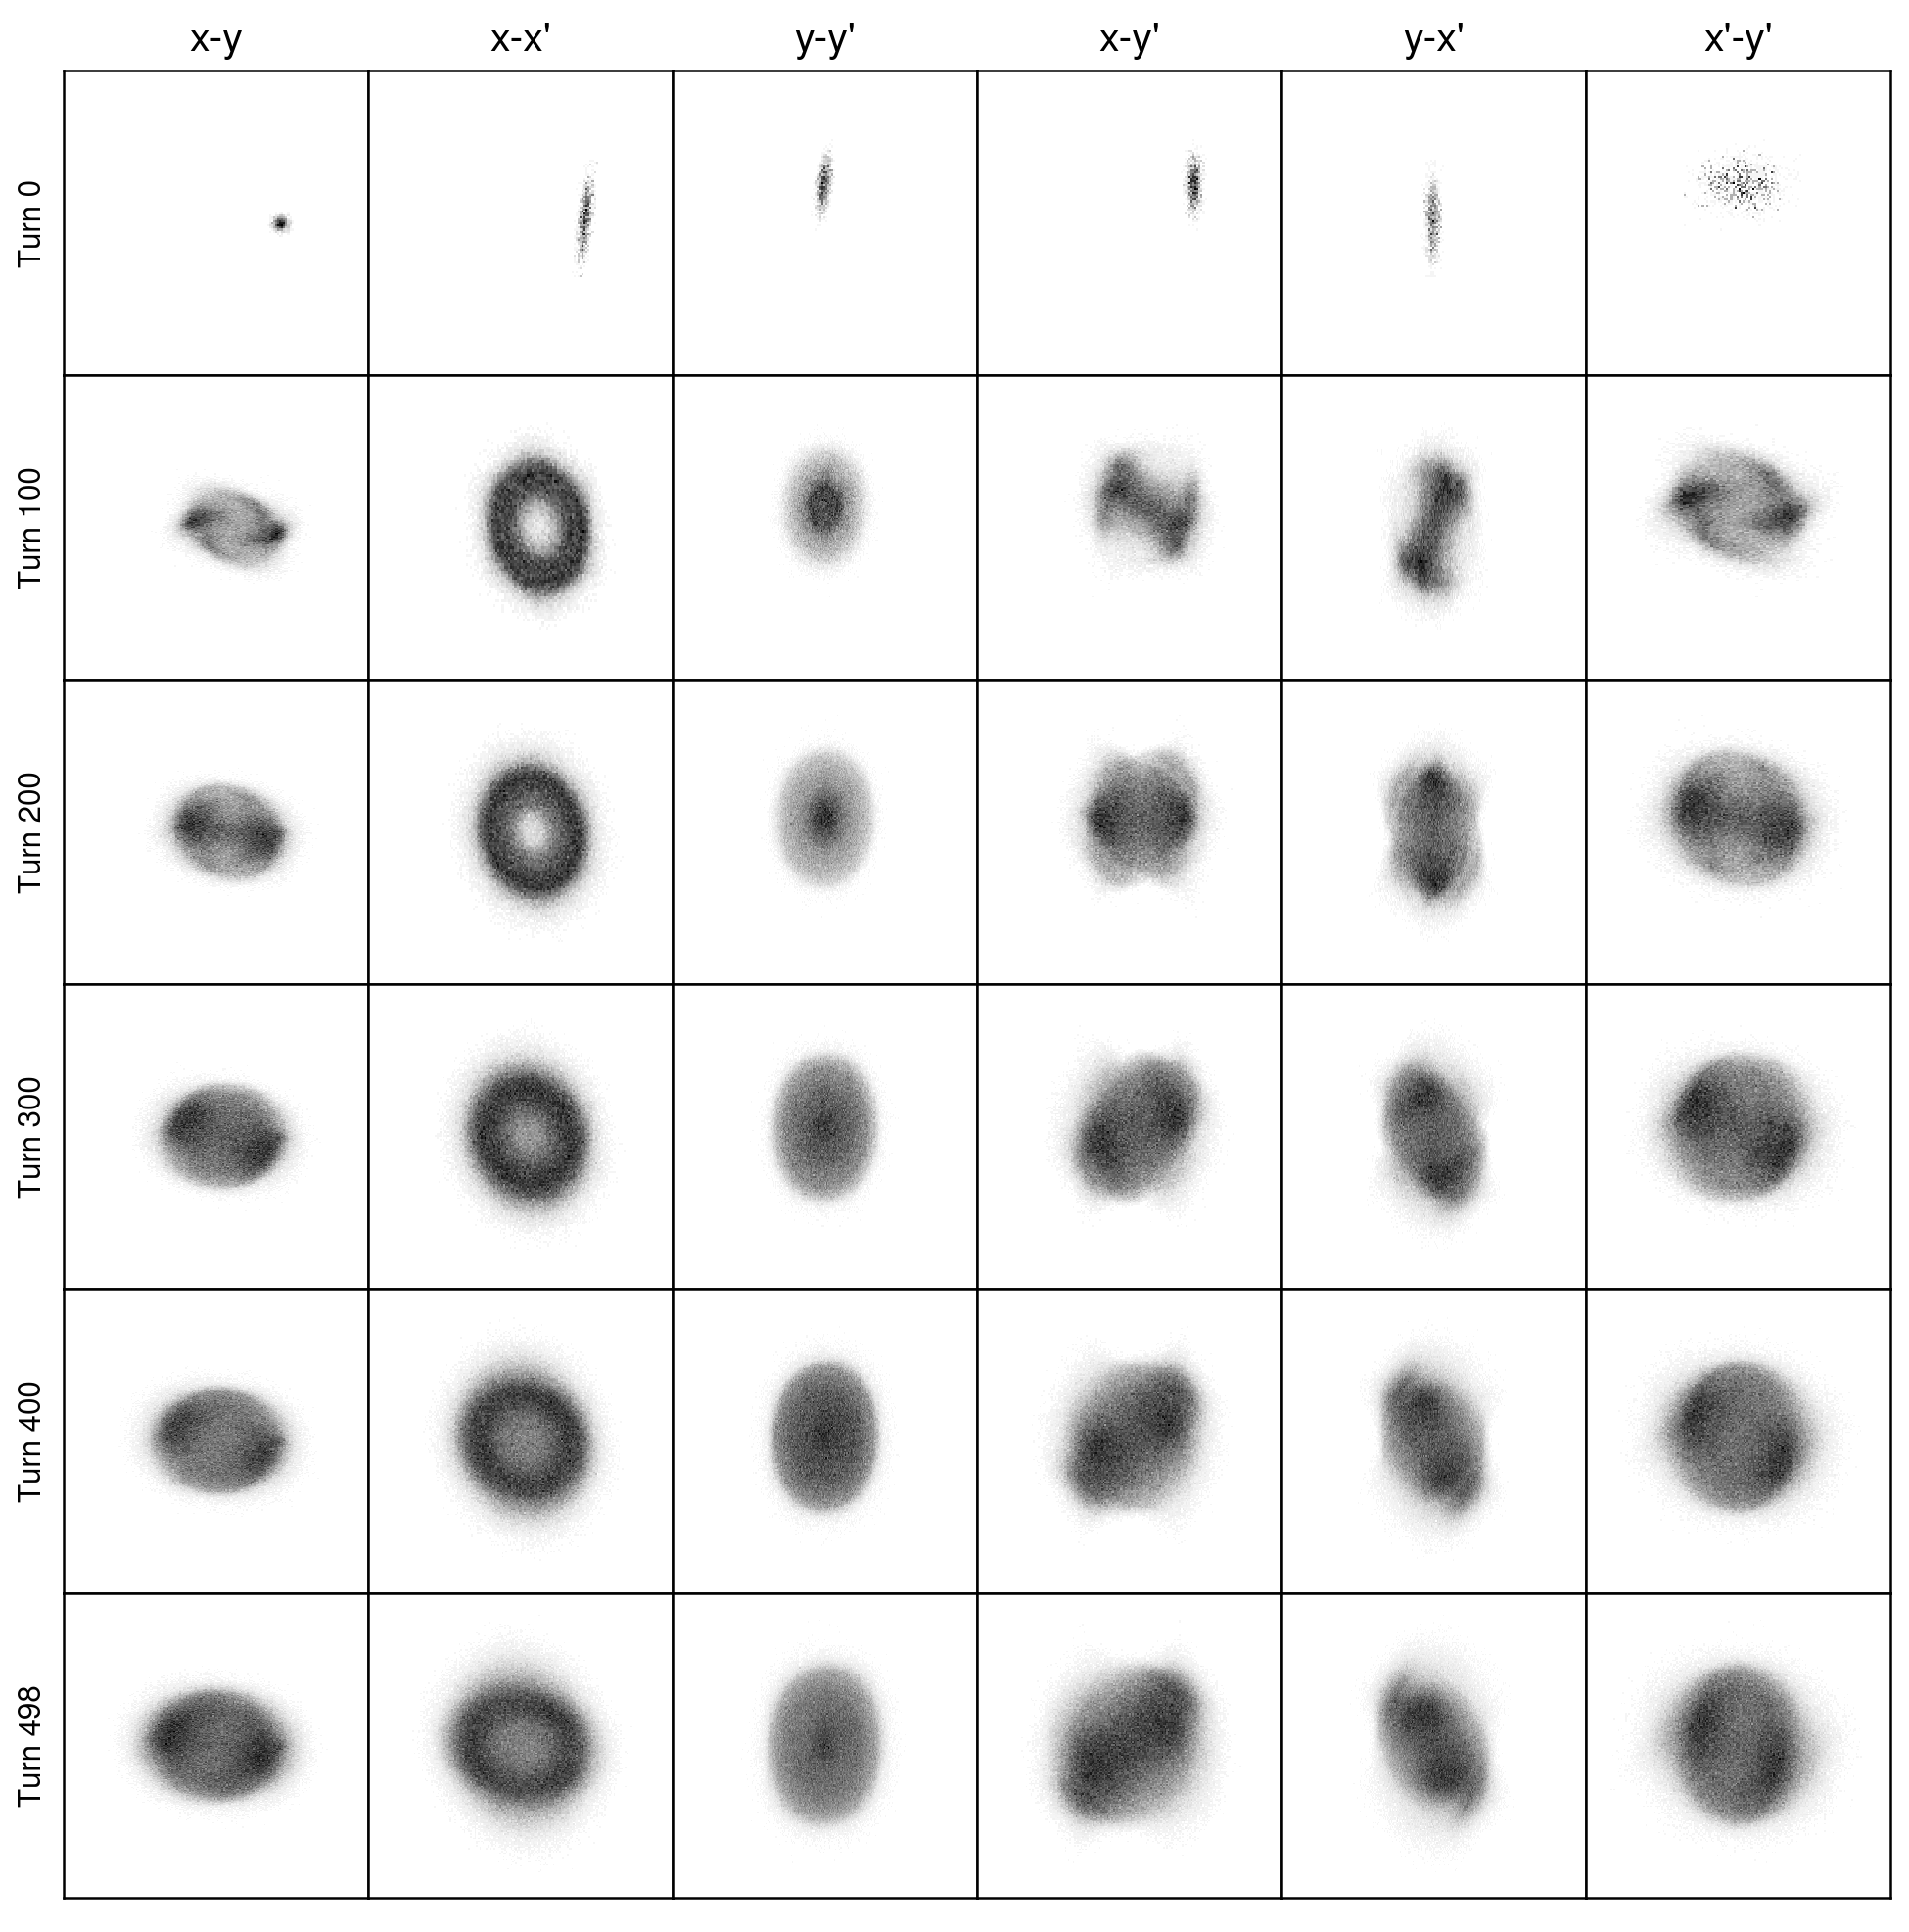
\includegraphics[width=\textwidth]{Images/chapter5/exp1b/sim_snapshots.png}
    \end{subfigure}
    \vfill
    \vspace*{1.0cm}
    \vfill
    \begin{subfigure}{0.7\textwidth}
        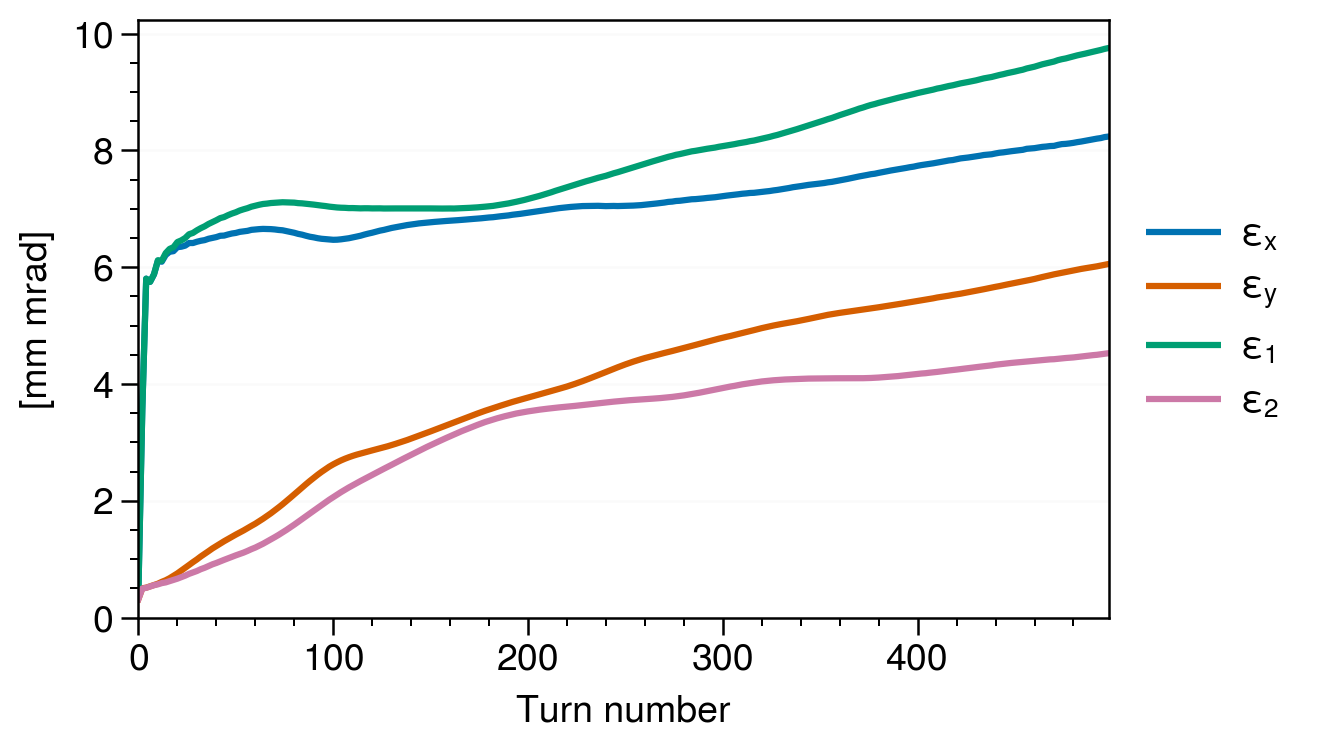
\includegraphics[width=\textwidth]{Images/chapter5/exp1b/sim_emittances.png}
    \end{subfigure}
    \caption{Simulation of Experiment 1b.}
    \label{fig:exp1b_sim}
\end{figure}
%
Keep in mind that the $\beta$ functions at the injection point are not exactly the same as in the experiment, so the exact values of the emittances are not expected to agree. The purpose of these simulations is to shed light on the measured data; we look for qualitative agreement in the emittance evolution, which appears to be present, as well as an explanation for the shape of the wire-scanner profiles through comparison with the 2D projections of the simulated distribution. Here, the $x$-$x'$ donut is clear in the simulation.


\section{Experiment 2}

In Experiment 2, the beam energy was lowered to 0.8 GeV for the first time. The closed orbit was able to reach the foil, and a maximum vertical slope of ${y'}_{max} \approx 1.1$ mrad was achieved. Although ${y'}_{max}$ is small, elliptical painting is possible with these settings. 

In the setup procedure, an optional step was listed: 3. Modify the injection region in some way to assist the injection kickers. There are several tricks that can be played to increase ${y'}_{max}$. One option would be to move the foil farther into the beam pipe, but this is undesired because it would require modification of the trajectory of the surviving hydrogen ions. Another option is to use the vertical orbit corrector dipoles in the injection region to increase the maximum vertical slope. This is not straightforward in reality because the correctors are already used to flatten the orbit during neutron production. There are two correctors before and after the foil. Our strategy was to manually change the first two correctors, then use the second two correctors and every other corrector in the ring to flatten the orbit (using an existing Orbit Correction application). There are four options for the sign of the changes applied to the first two correctors: $\uparrow\uparrow$, $\uparrow\downarrow$, $\downarrow\uparrow$, $\downarrow\downarrow$. For each option, a small change was applied to the dipole currents and the injection kickers were asked to maximize the vertical slope at the foil. This did not work; modifying the correctors lead to significant closed-orbit waves throughout the ring that could not be flattened. The use of orbit correctors was left as a future optimization. 

The remaining free parameters are the beam intensity and the maximum horizontal position $x_{max}$. Assuming $\alpha \approx 0$ at the injection point, the ratio of painted emittances is
%
\begin{equation}
    \frac{\varepsilon_y}{\varepsilon_x} \approx 
    \beta_x \beta_y \left(\frac{{y'}_{max}}{x_{max}}\right)^2 
\end{equation}
%
It is known that the matched solution with space charge has equal emittances. In simulations, this can easily be achieved since the $\beta$ functions are known. In reality, the exact $\beta$ functions are unknown. The model $\beta$ functions at the injection point are both near 10 mm/mrad; for $y'_{max}$ = 1 mrad, this would require $x_{max}$ = 10 mm — a small beam. But we must keep in mind that the ratio is quite sensitive to changes in $\beta_{x, y}$; for example, $\beta_x$ = $\beta_y$ = 11 m/rad would produce $\varepsilon_y / \varepsilon_x \approx 1.5$. We decided to use $x_{max}$ = 21 mm. The beam intensity was kept at 500 injected turns, or roughly $0.75 \times 10^{14}$ protons.

The measured wire-scanner profiles are shown in Fig.~\ref{fig:exp2_wsmeas}, and the reconstructed emittances and covariance ellipses at BPM17 are shown in Fig.~\ref{fig:exp2_emittances}.
%
\begin{figure}[!p]
    \centering
    \begin{subfigure}{\textwidth}
        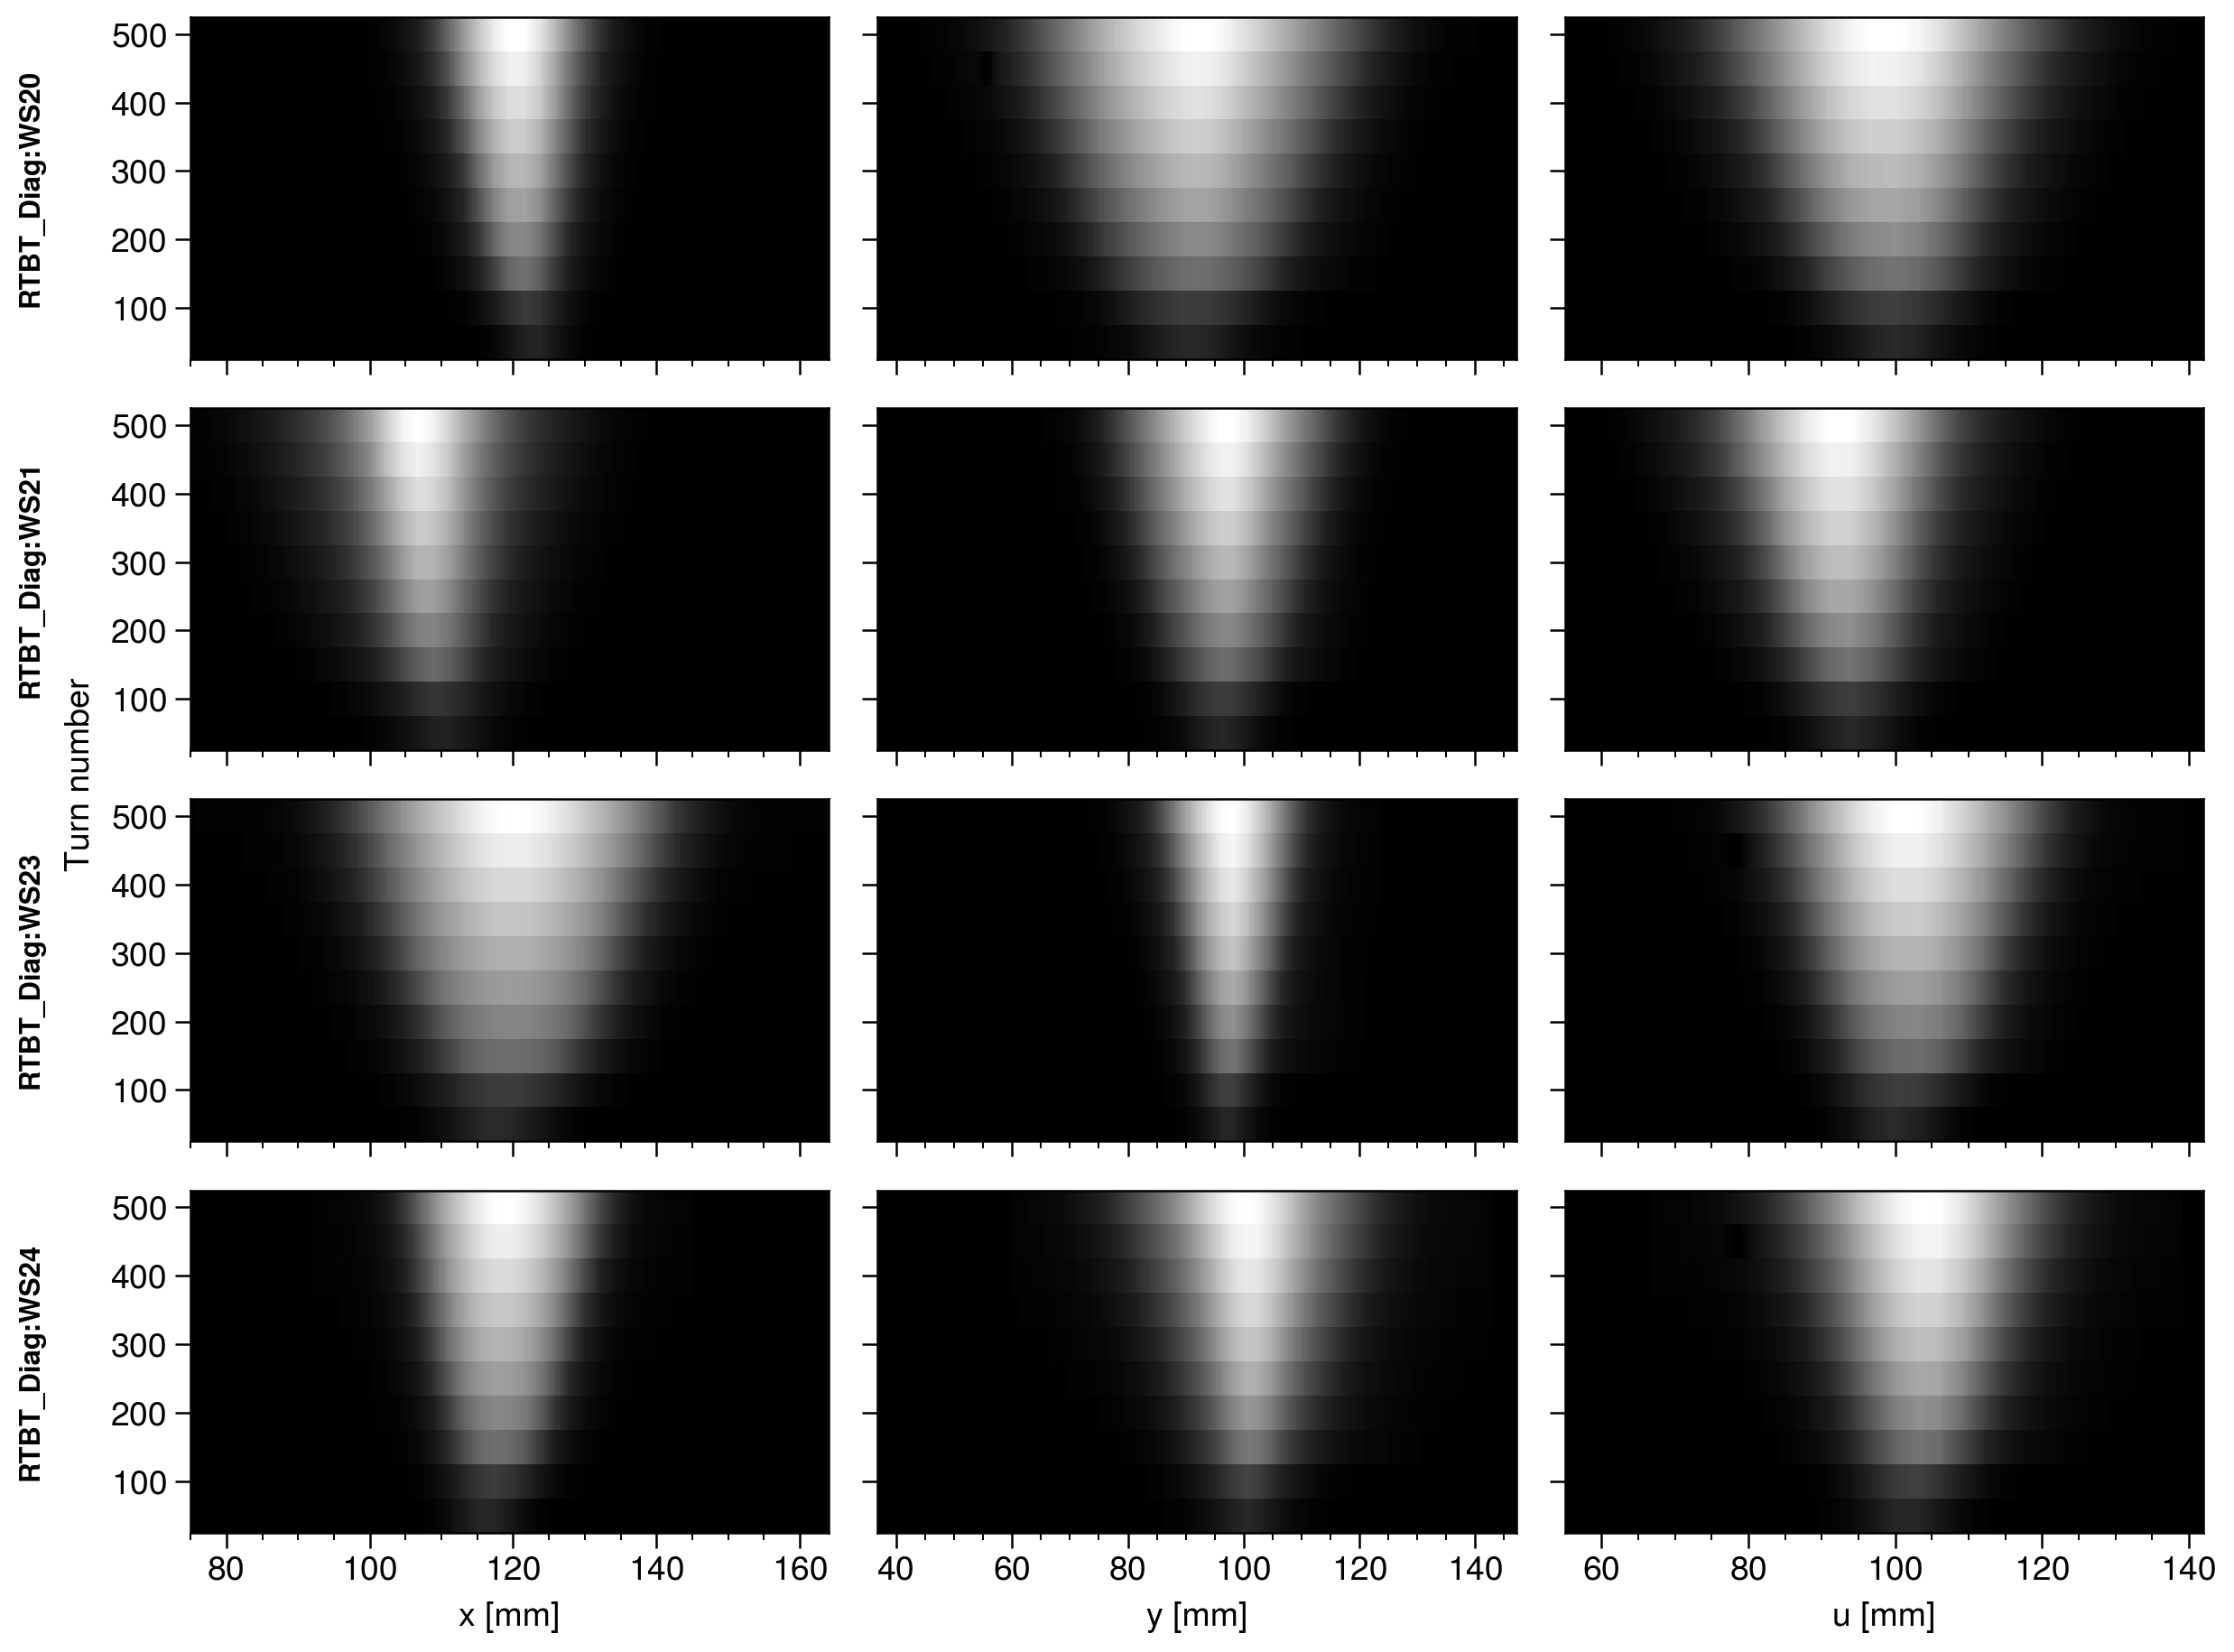
\includegraphics[width=\textwidth]{Images/chapter5/exp2/waterfall.png}
    \end{subfigure}
    \vfill
    \vspace*{1.25cm}
    \vfill
    \begin{subfigure}{\textwidth}
        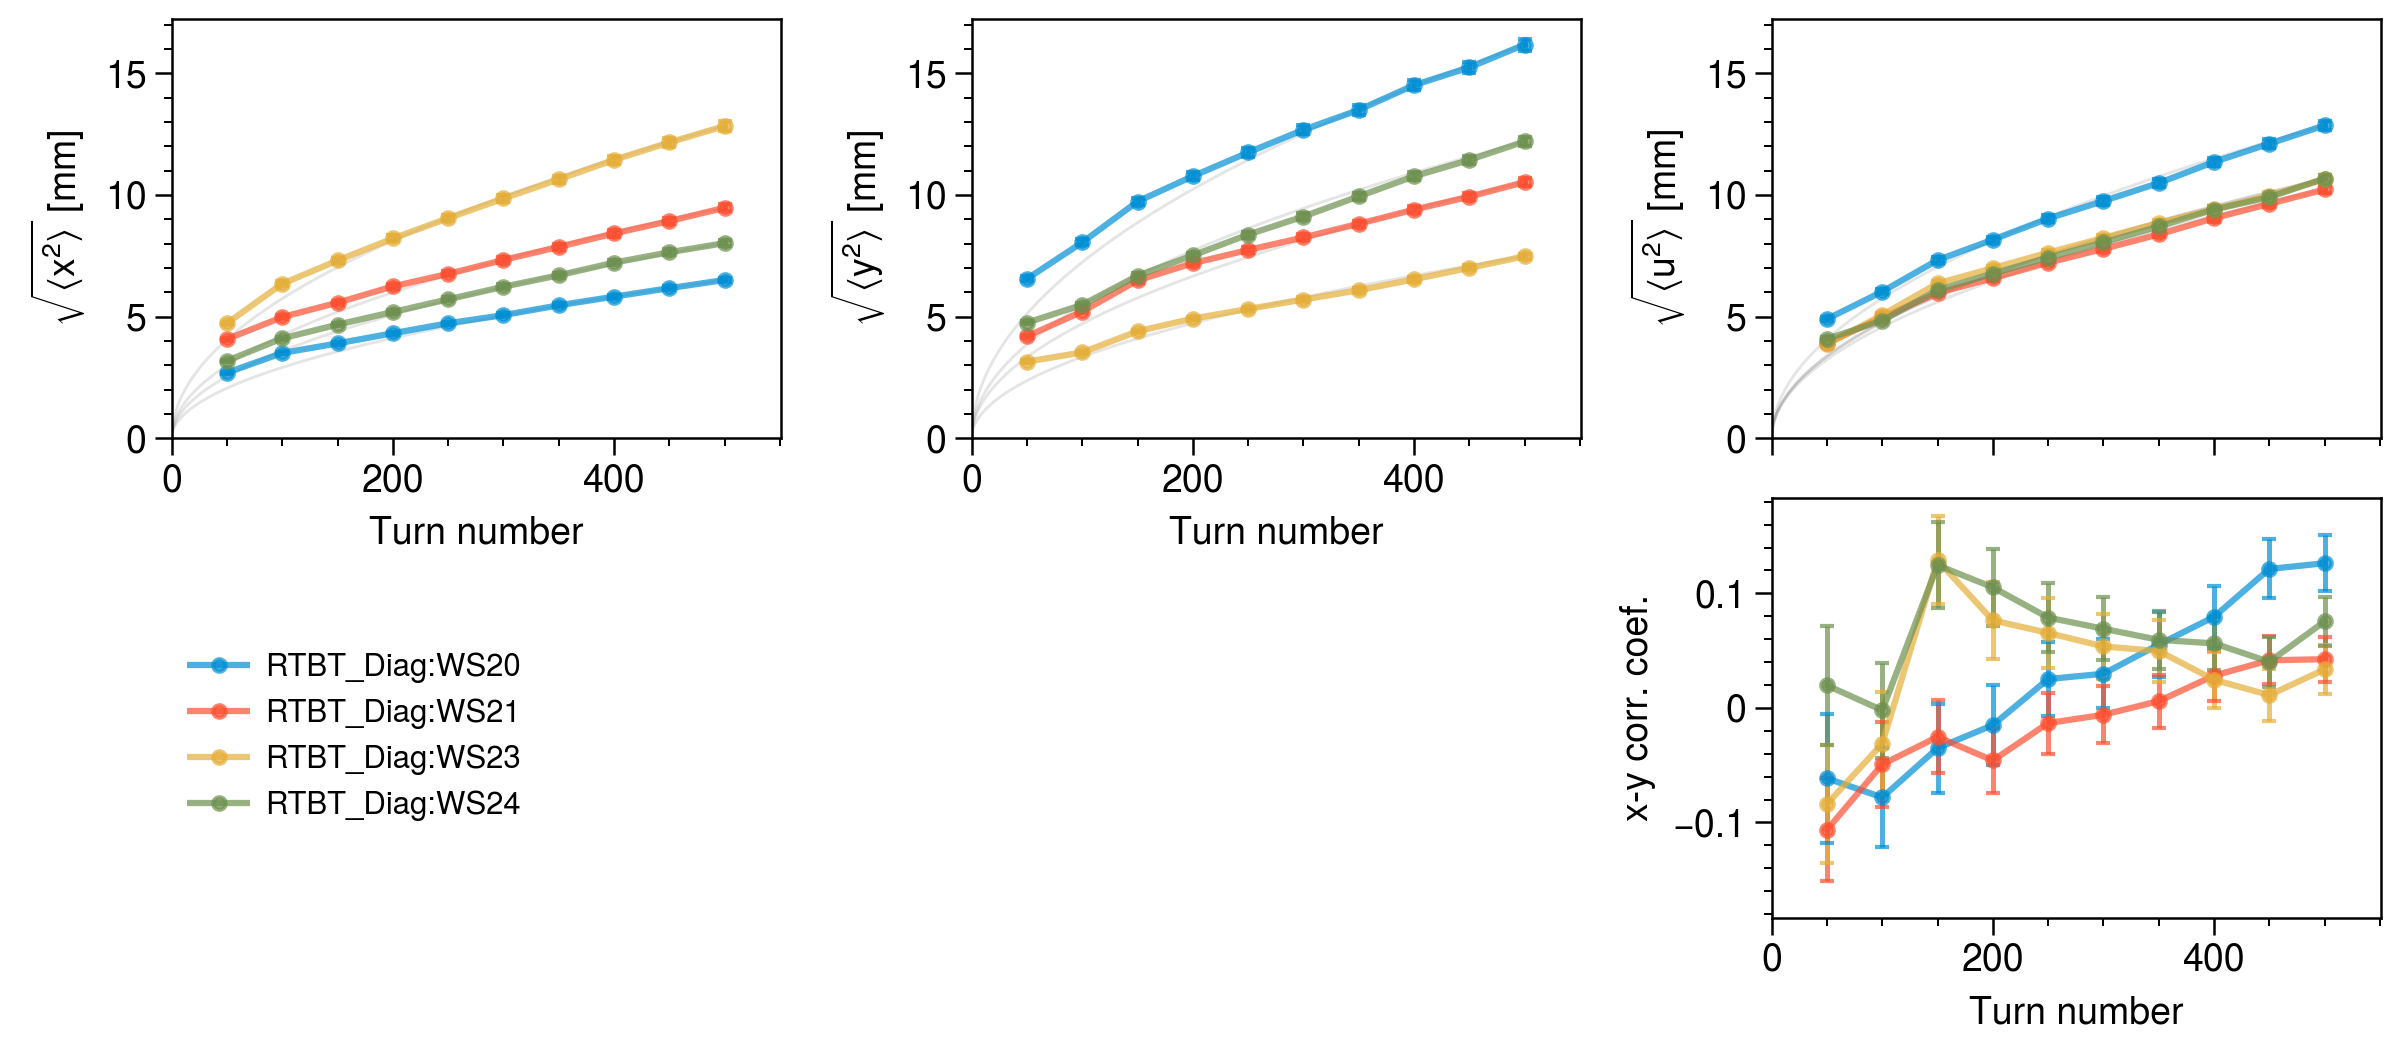
\includegraphics[width=\textwidth]{Images/chapter5/exp2/rms.png}
    \end{subfigure}
    \caption{Measured wire-scanner profiles during injection from Experiment 2.}
    \label{fig:exp2_wsmeas}
\end{figure}
%
%
\begin{figure}[!p]
    \centering
    \begin{subfigure}{0.6\textwidth}
        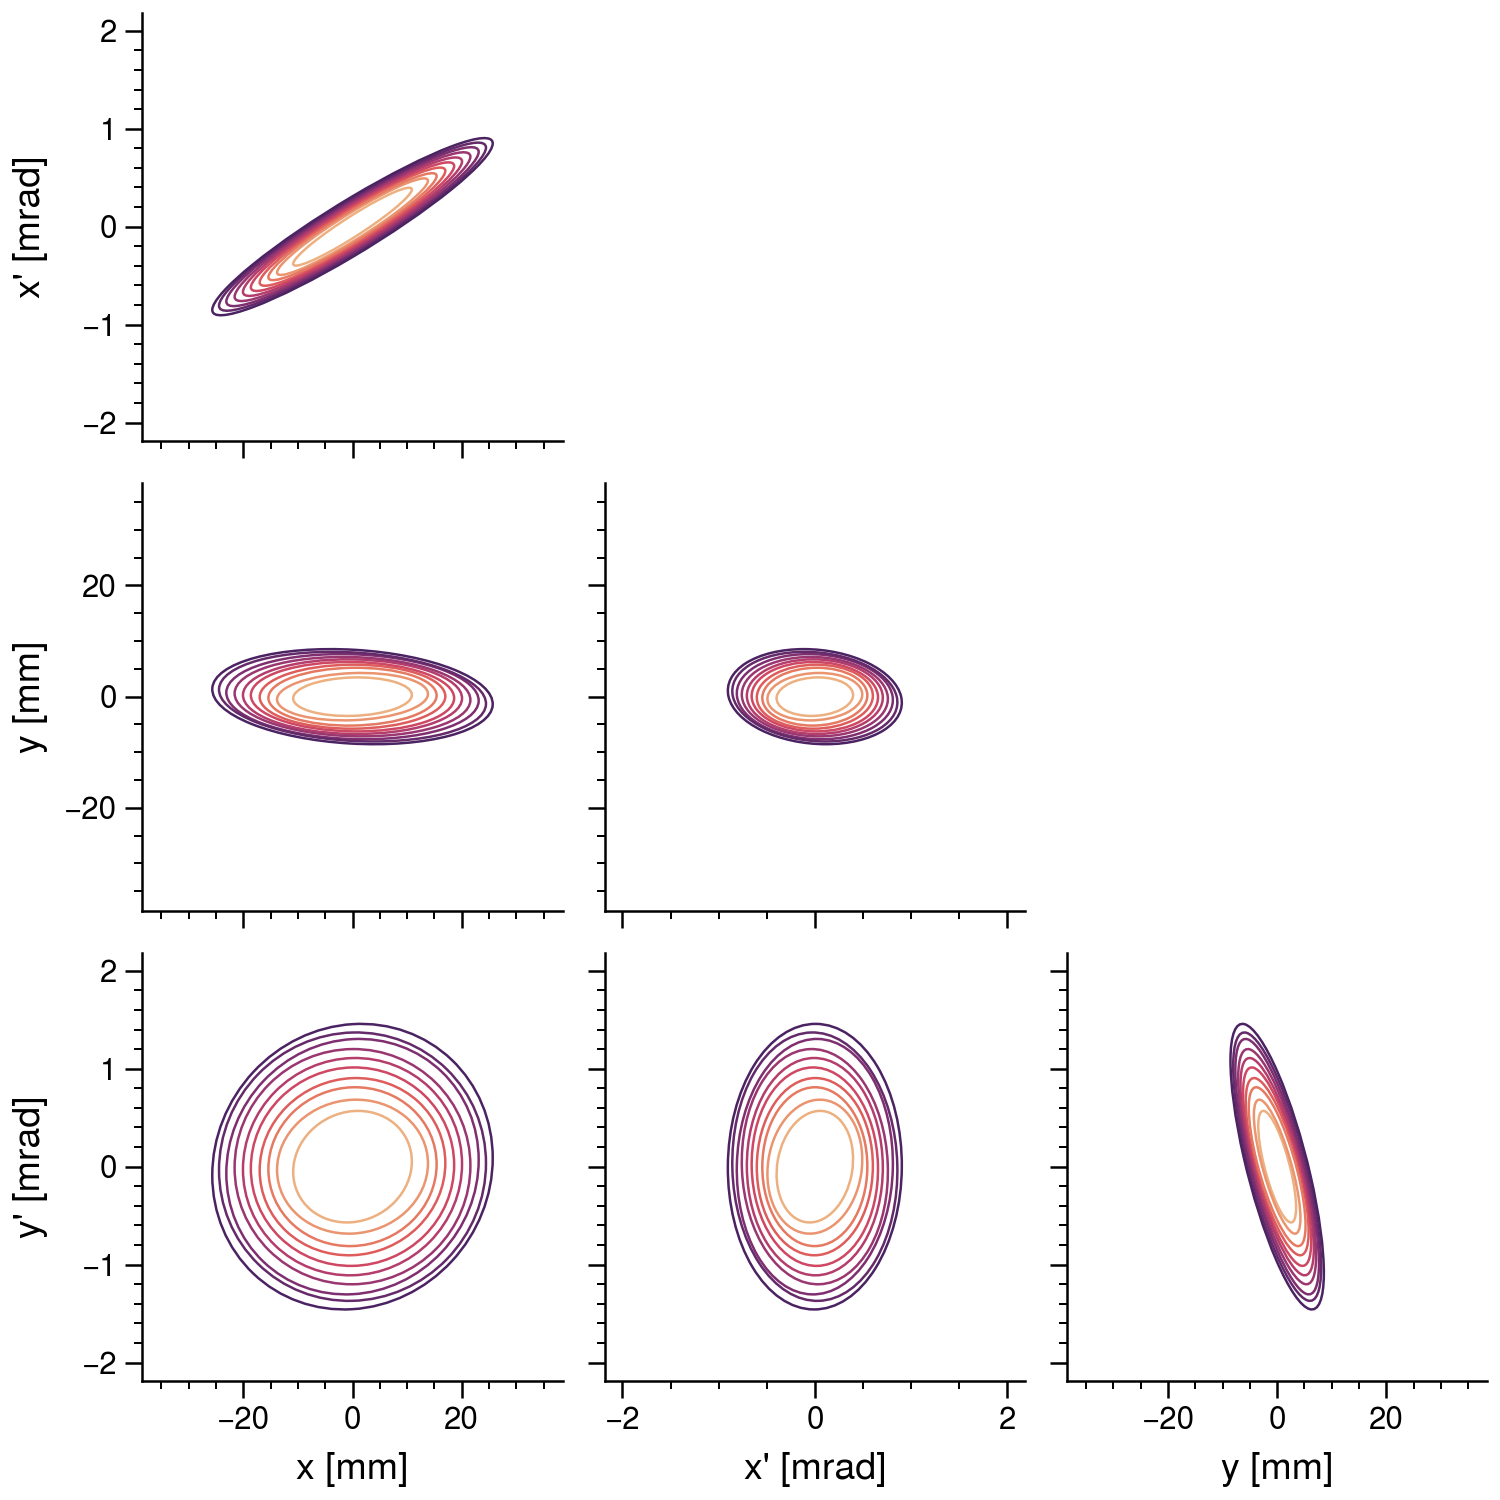
\includegraphics[width=\textwidth]{Images/chapter5/exp2/corner.png}
    \end{subfigure}
    \hfill
    \begin{subfigure}[t]{0.39\textwidth}
        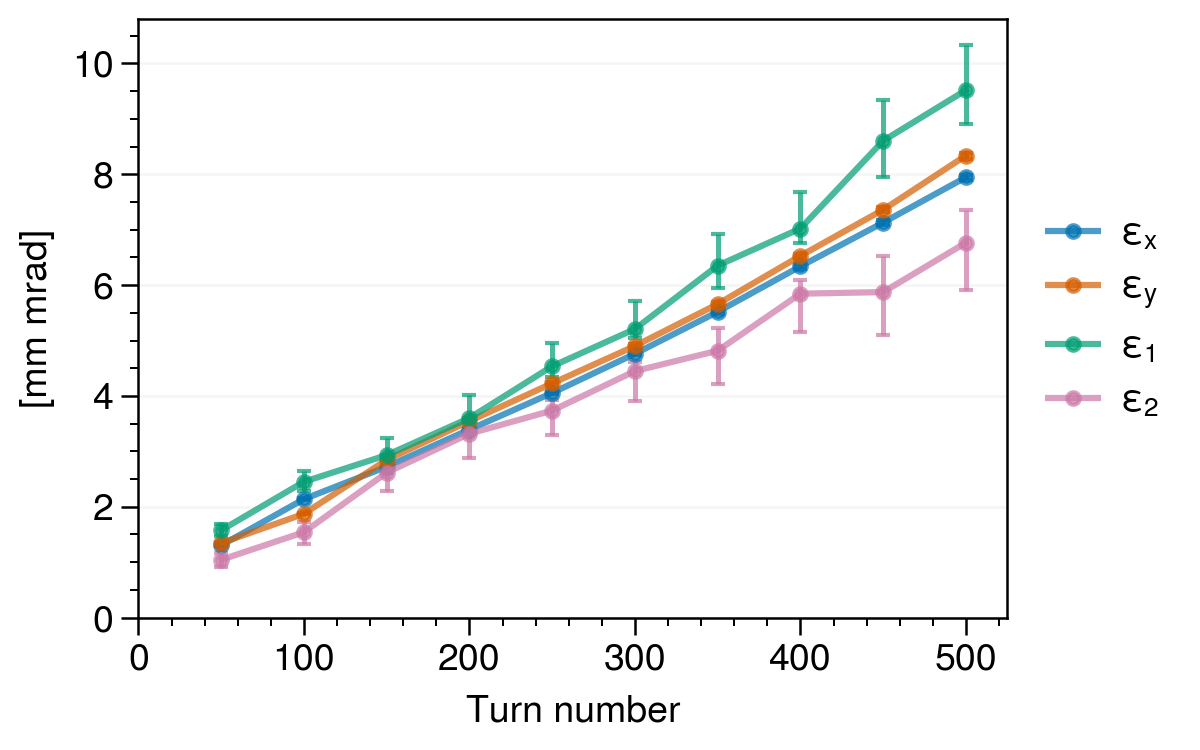
\includegraphics[width=\textwidth]{Images/chapter5/exp2/emittances.png}
    \end{subfigure}
    \caption{Reconstructed emittances and covariance ellipses from Experiment 2.}
    \label{fig:exp2_emittances}
\end{figure}
%
The apparent emittances increase linearly from a small initial value, as desired. The intrinsic emittances begin to split, although not by much, at the end of injection.

A simulation of this case is shown in Fig.~\ref{fig:exp2_sim}.
%
\begin{figure}[!p]
    \centering
    \begin{subfigure}{0.85\textwidth}
        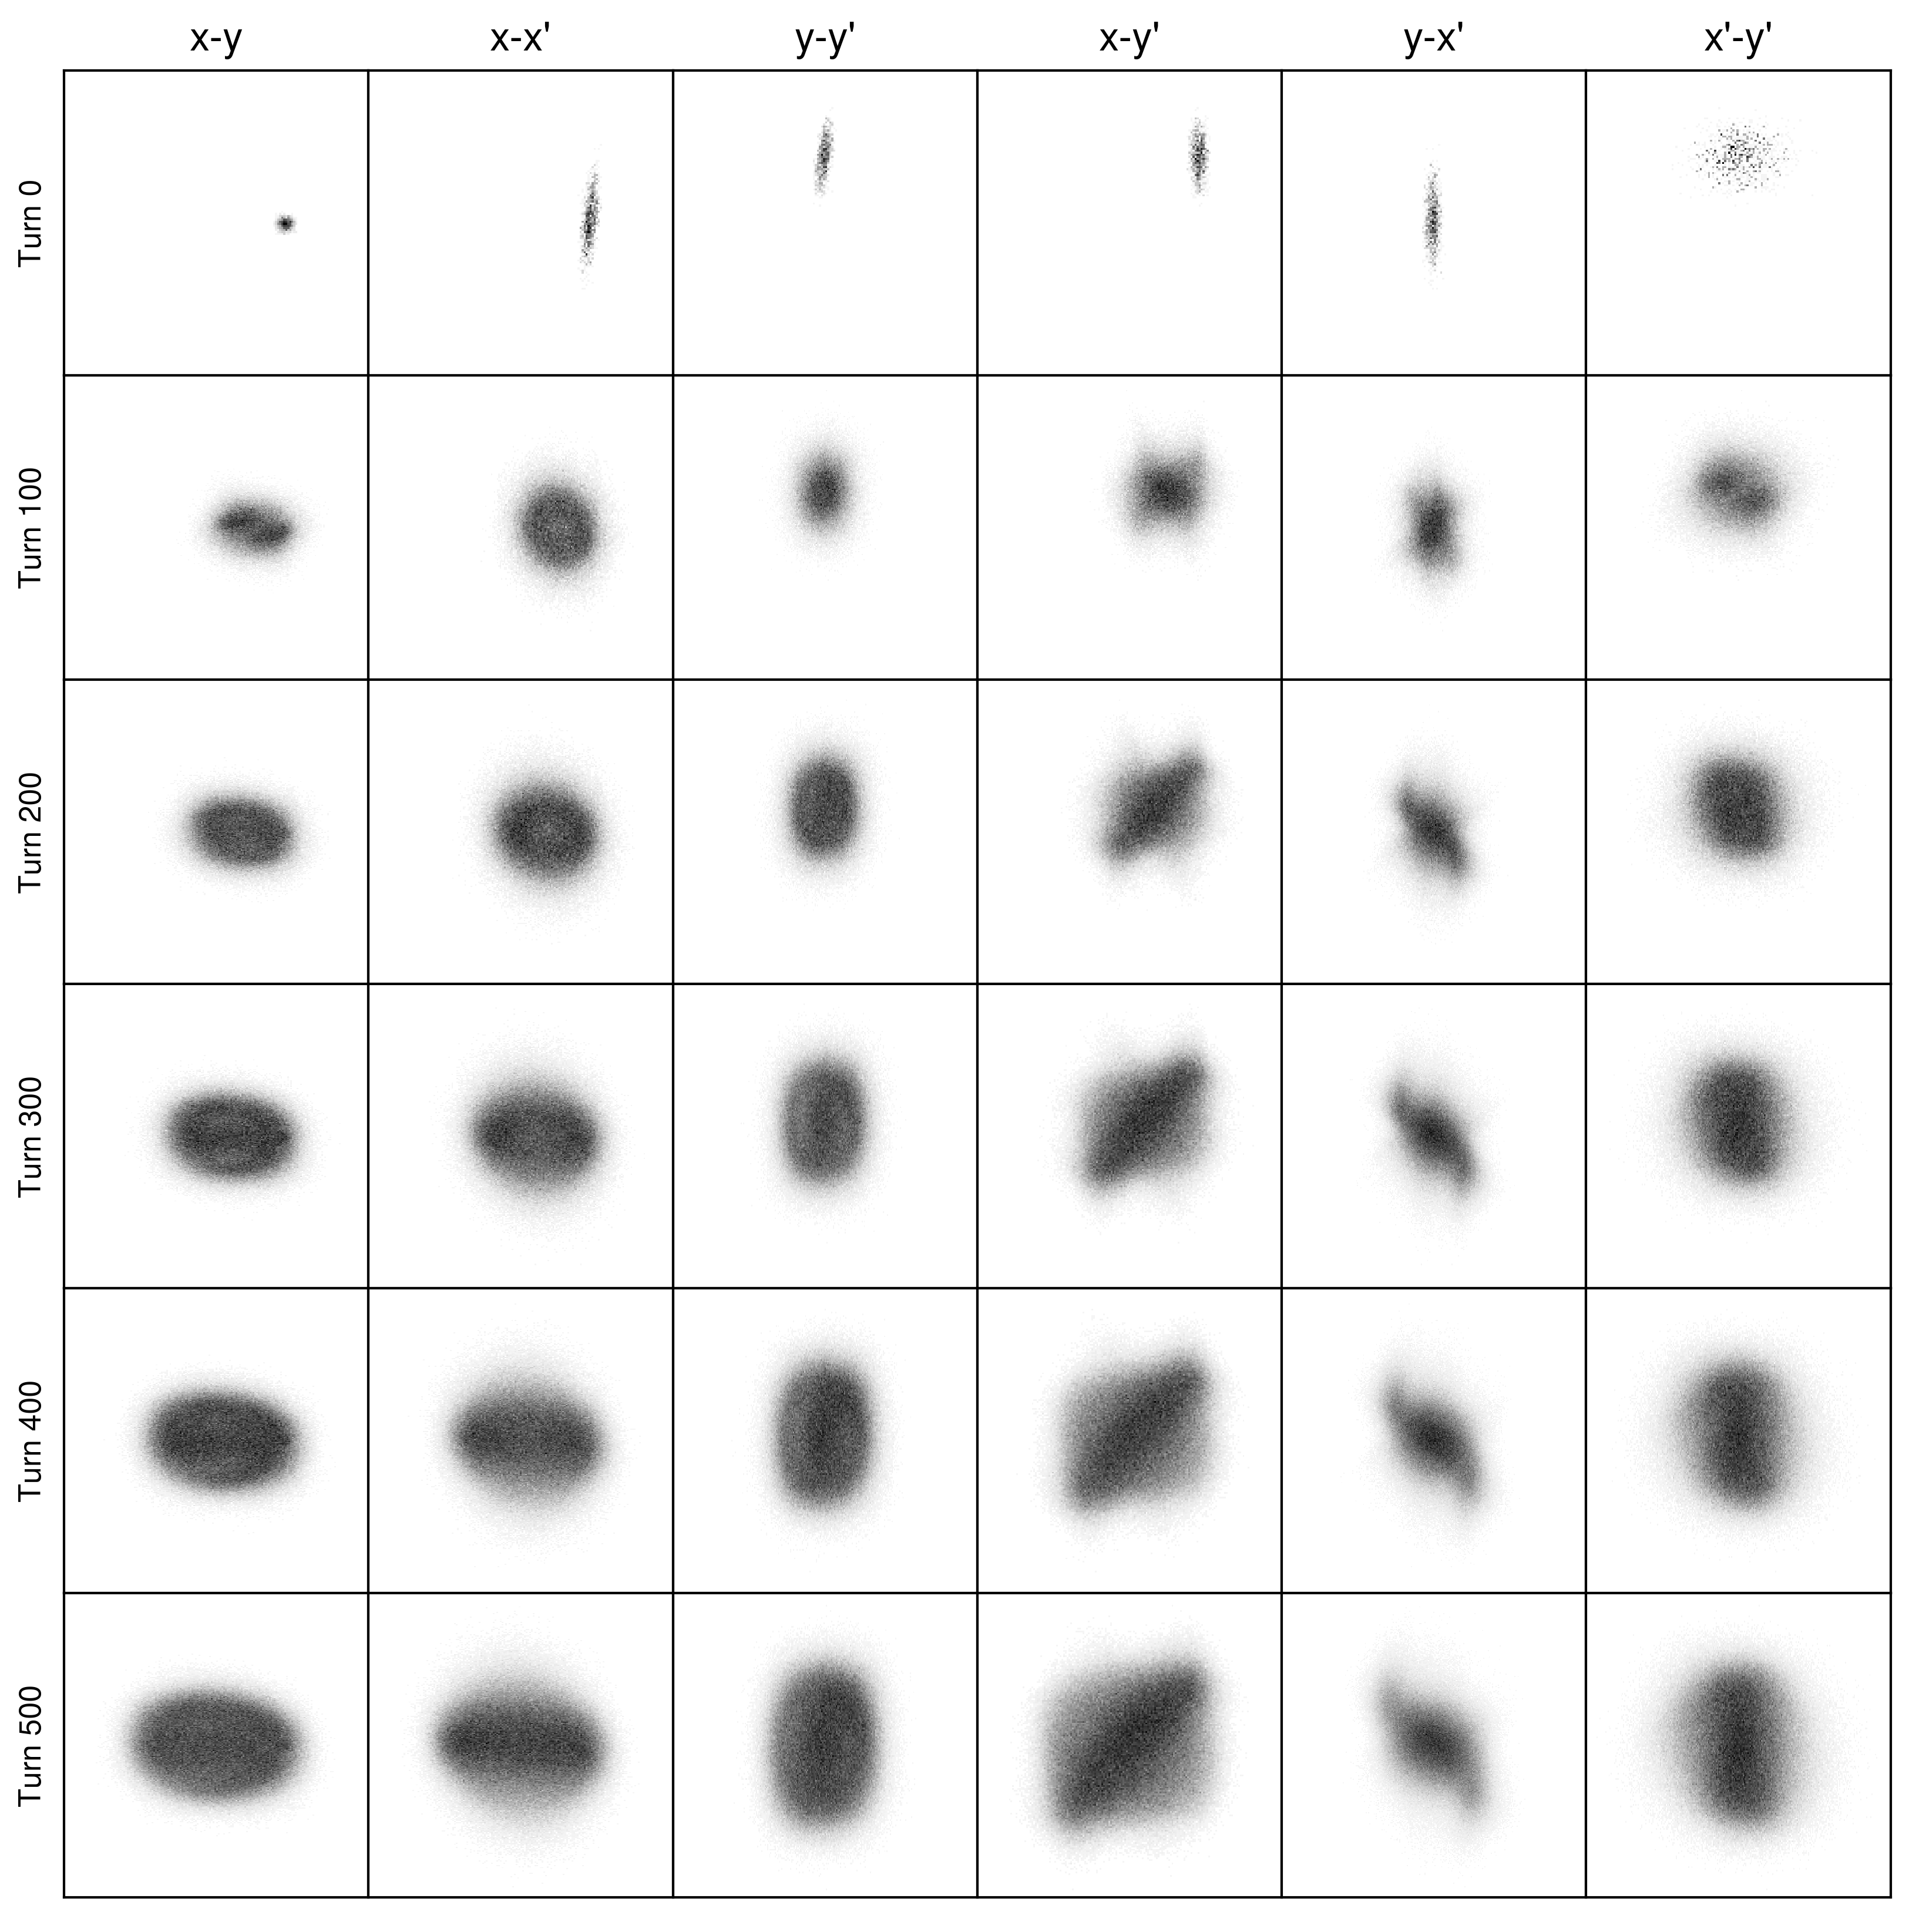
\includegraphics[width=\textwidth]{Images/chapter5/exp2/sim_snapshots.png}
    \end{subfigure}
    \vfill
    \vspace*{1.0cm}
    \vfill
    \begin{subfigure}{0.7\textwidth}
        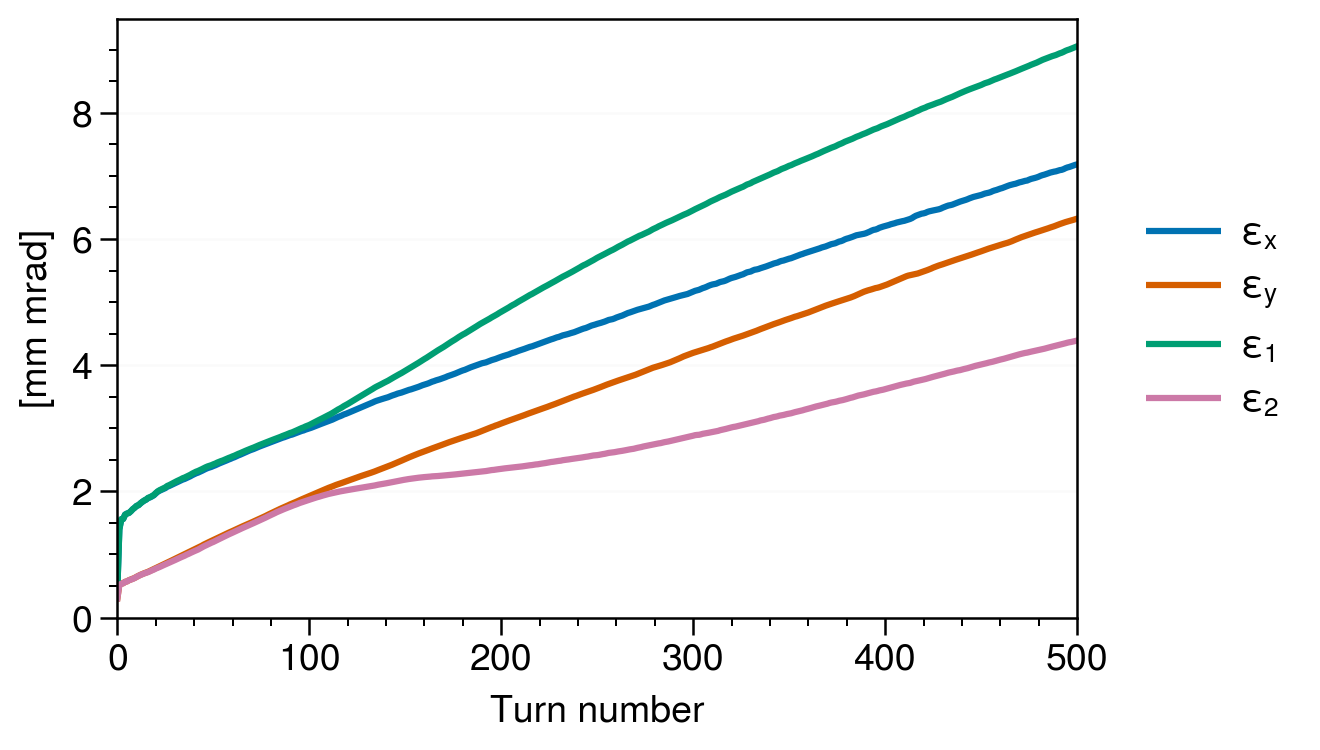
\includegraphics[width=\textwidth]{Images/chapter5/exp2/sim_emittances.png}
    \end{subfigure}
    \caption{Simulation of Experiment 2.}
    \label{fig:exp2_sim}
\end{figure}
%
Notice that $\varepsilon_2$ begins to flatten after turn 100, but does not remain flat. Although the final $x$-$y'$ projection has a higher density along the painting path, the linear correlation is significantly blurred. This is likely because space charge has a strong effect on the evolution at this intensity, energy, and beam size. Nonetheless, the simulation predicts a ``better" result than what was measured.



\section{Experiment 3}

The same setup for Experiment 2 was repeated in Experiment 3. One difference was that the beam length was increased from roughly 30/64 of the ring length to 45/64 of the ring length to better approximate a coasting beam. At the start of the experiment, the beam intensity and beam size were varied; at each setting, the covariance matrix of the final distribution were reconstructed using four wire-scanner profiles. The results are shown in Fig.~\ref{fig:exp3_search}. (The intensities are not exact; they are obtained by multiplying the nominal minipulse intensity by the number of injected turns.) Collective effects clearly have an effect on the final distribution. It is somewhat surprising that the split in the intrinsic emittances increased with the beam intensity. 
%
\begin{figure}[!p]
    \centering
    \vspace*{1.0cm}
    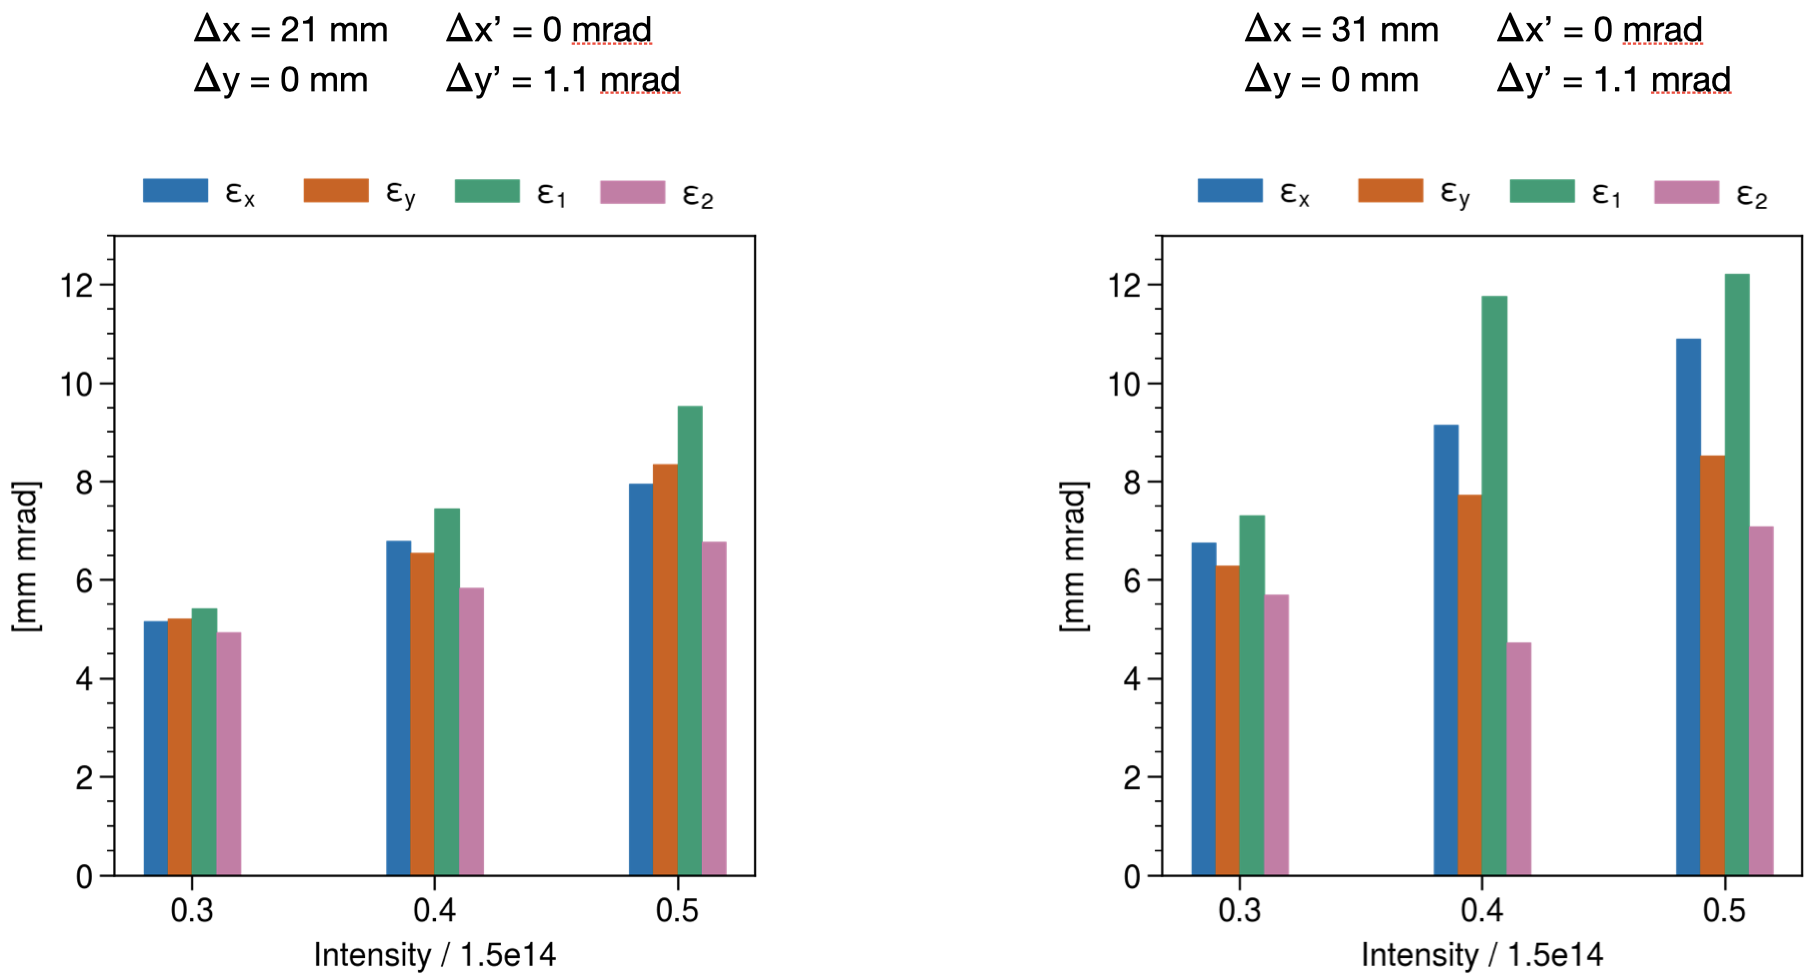
\includegraphics[width=\textwidth]{Images/chapter5/exp3/search.png}
    \caption{Measured emittances vs. beam intensity for two sets of injected coordinates. [TO DO: ADD ERROR BARS]}
    \label{fig:exp3_search}
    \vspace*{1.0cm}
\end{figure}
%
The middle cluster in the right subplot was identified as the most interesting case, and the measurement process of the previous two experiments was repeated — see Fig.~\ref{fig:exp3_wsmeas} and Fig.~\ref{fig:exp3_emittances}.
%
\begin{figure}[!p]
    \centering
    \begin{subfigure}{\textwidth}
        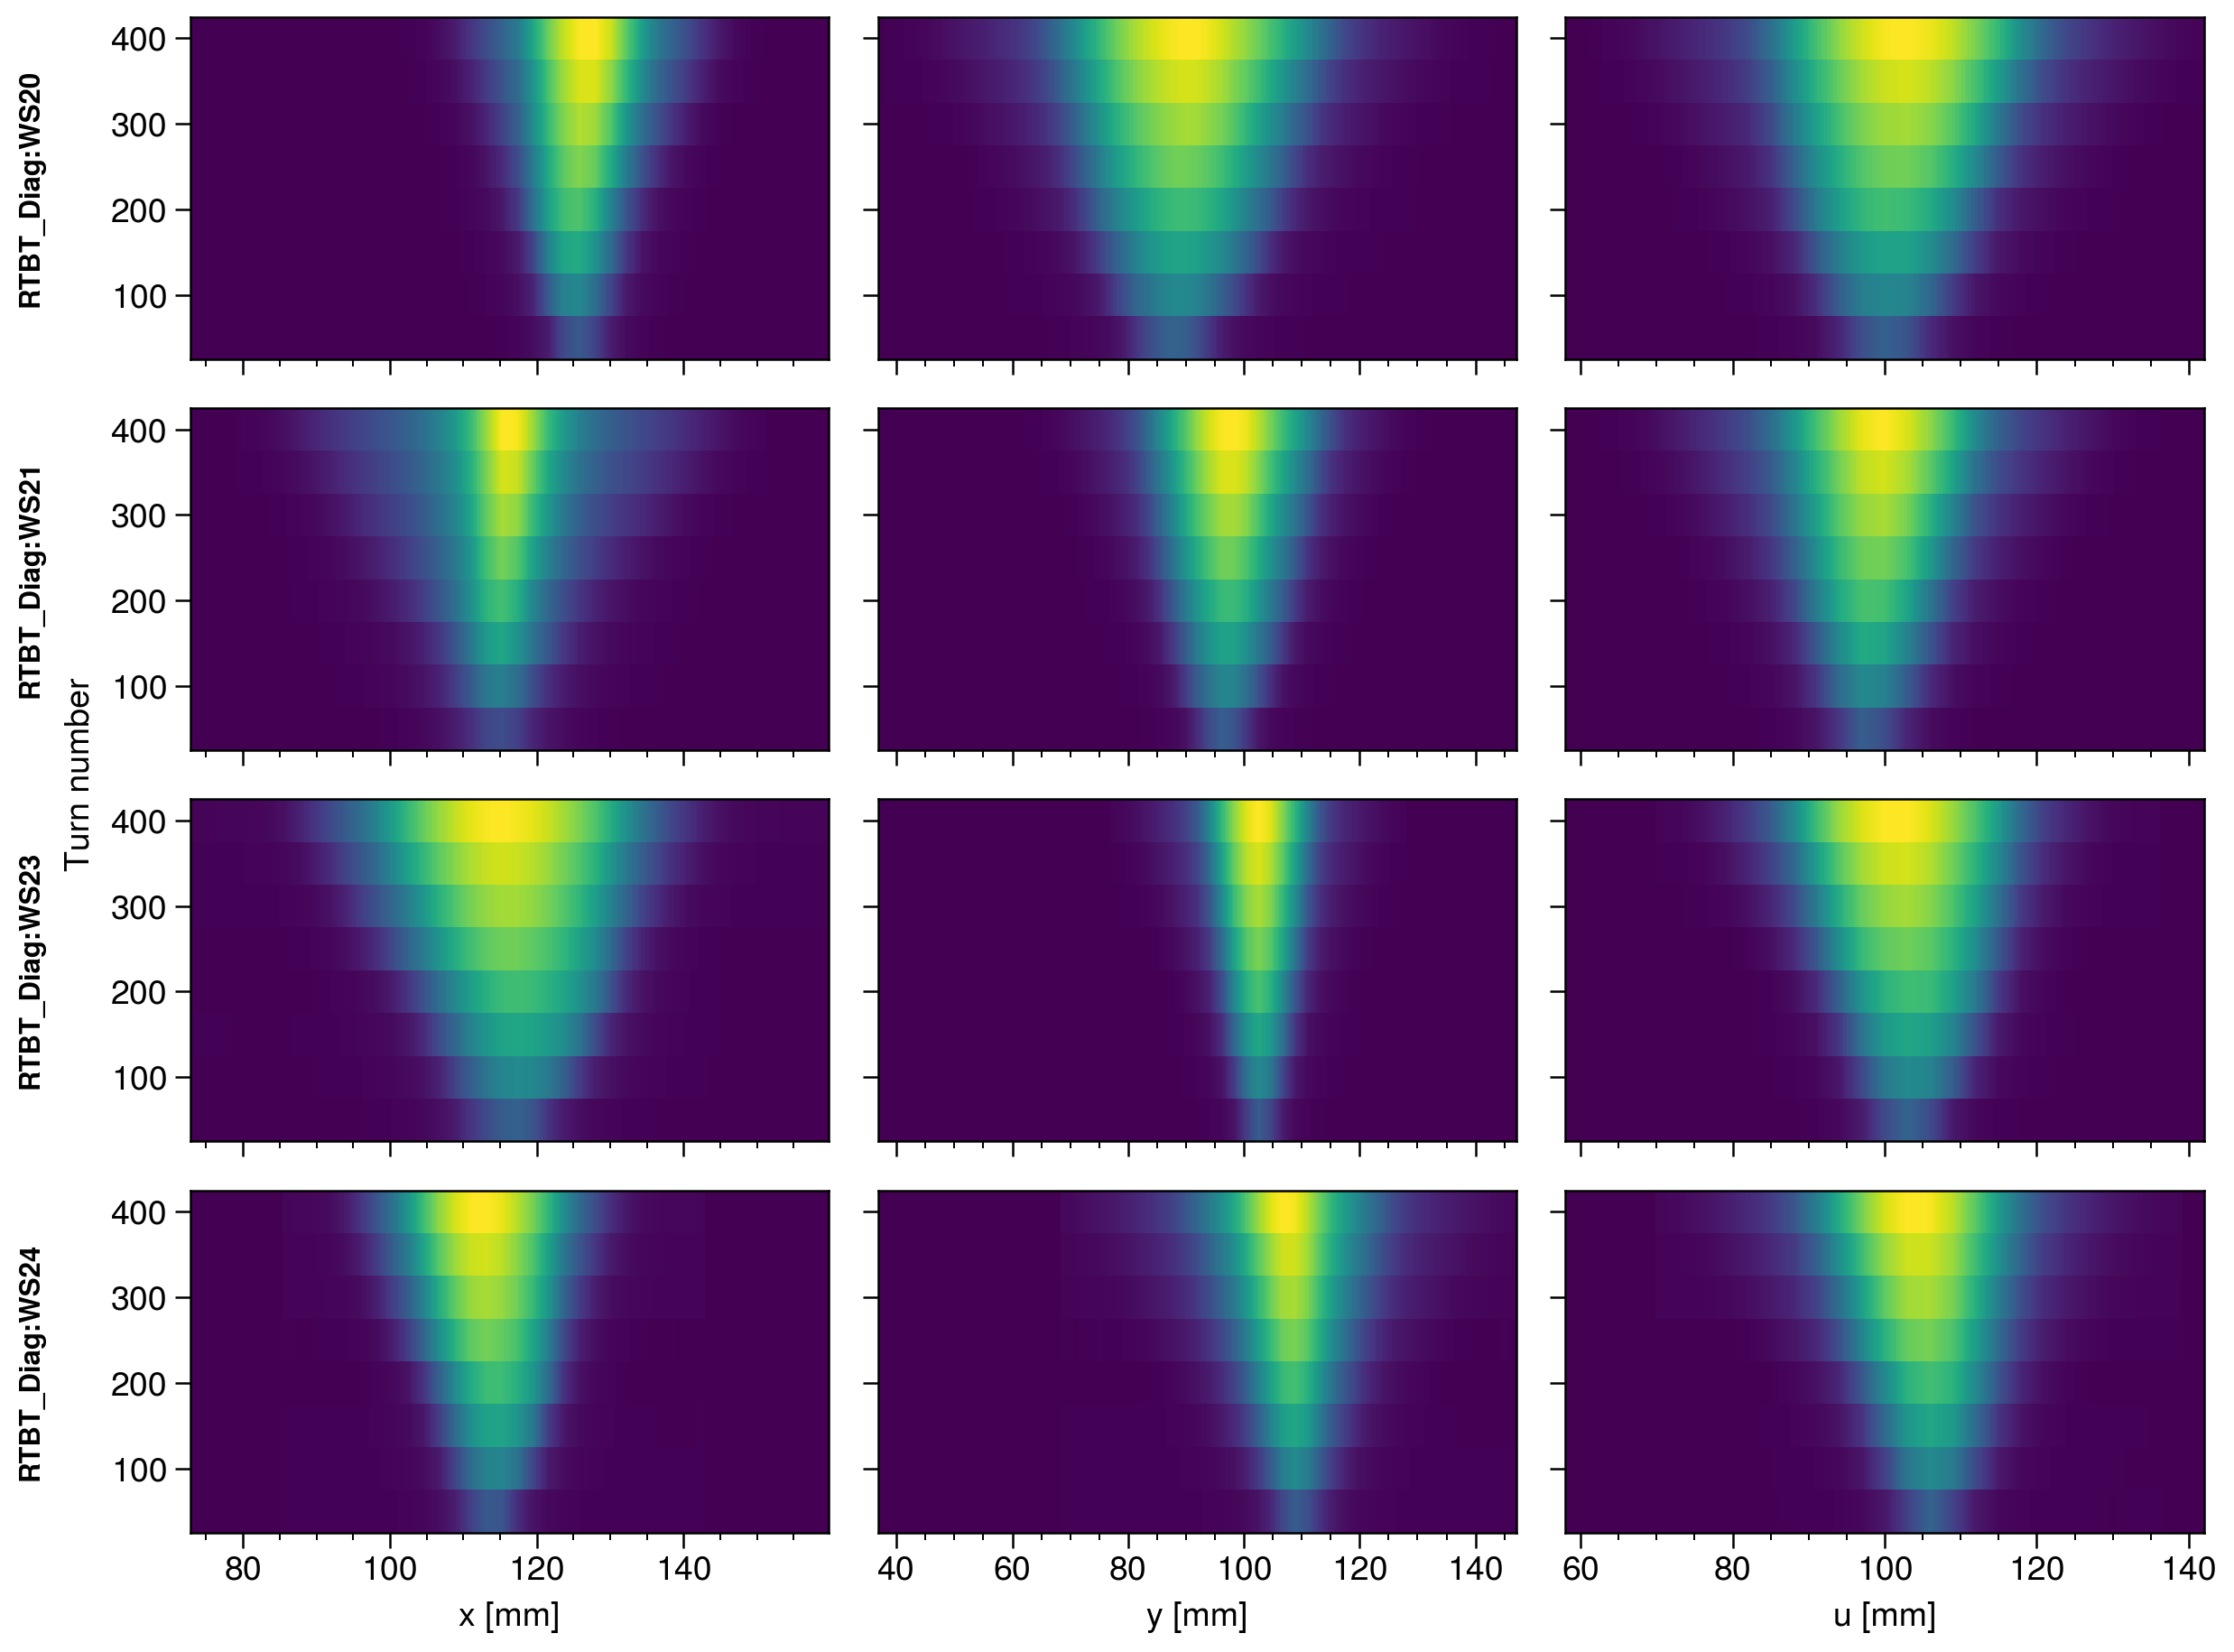
\includegraphics[width=\textwidth]{Images/chapter5/exp3/waterfall.png}
    \end{subfigure}
    \vfill
    \vspace*{1.25cm}
    \vfill
    \begin{subfigure}{\textwidth}
        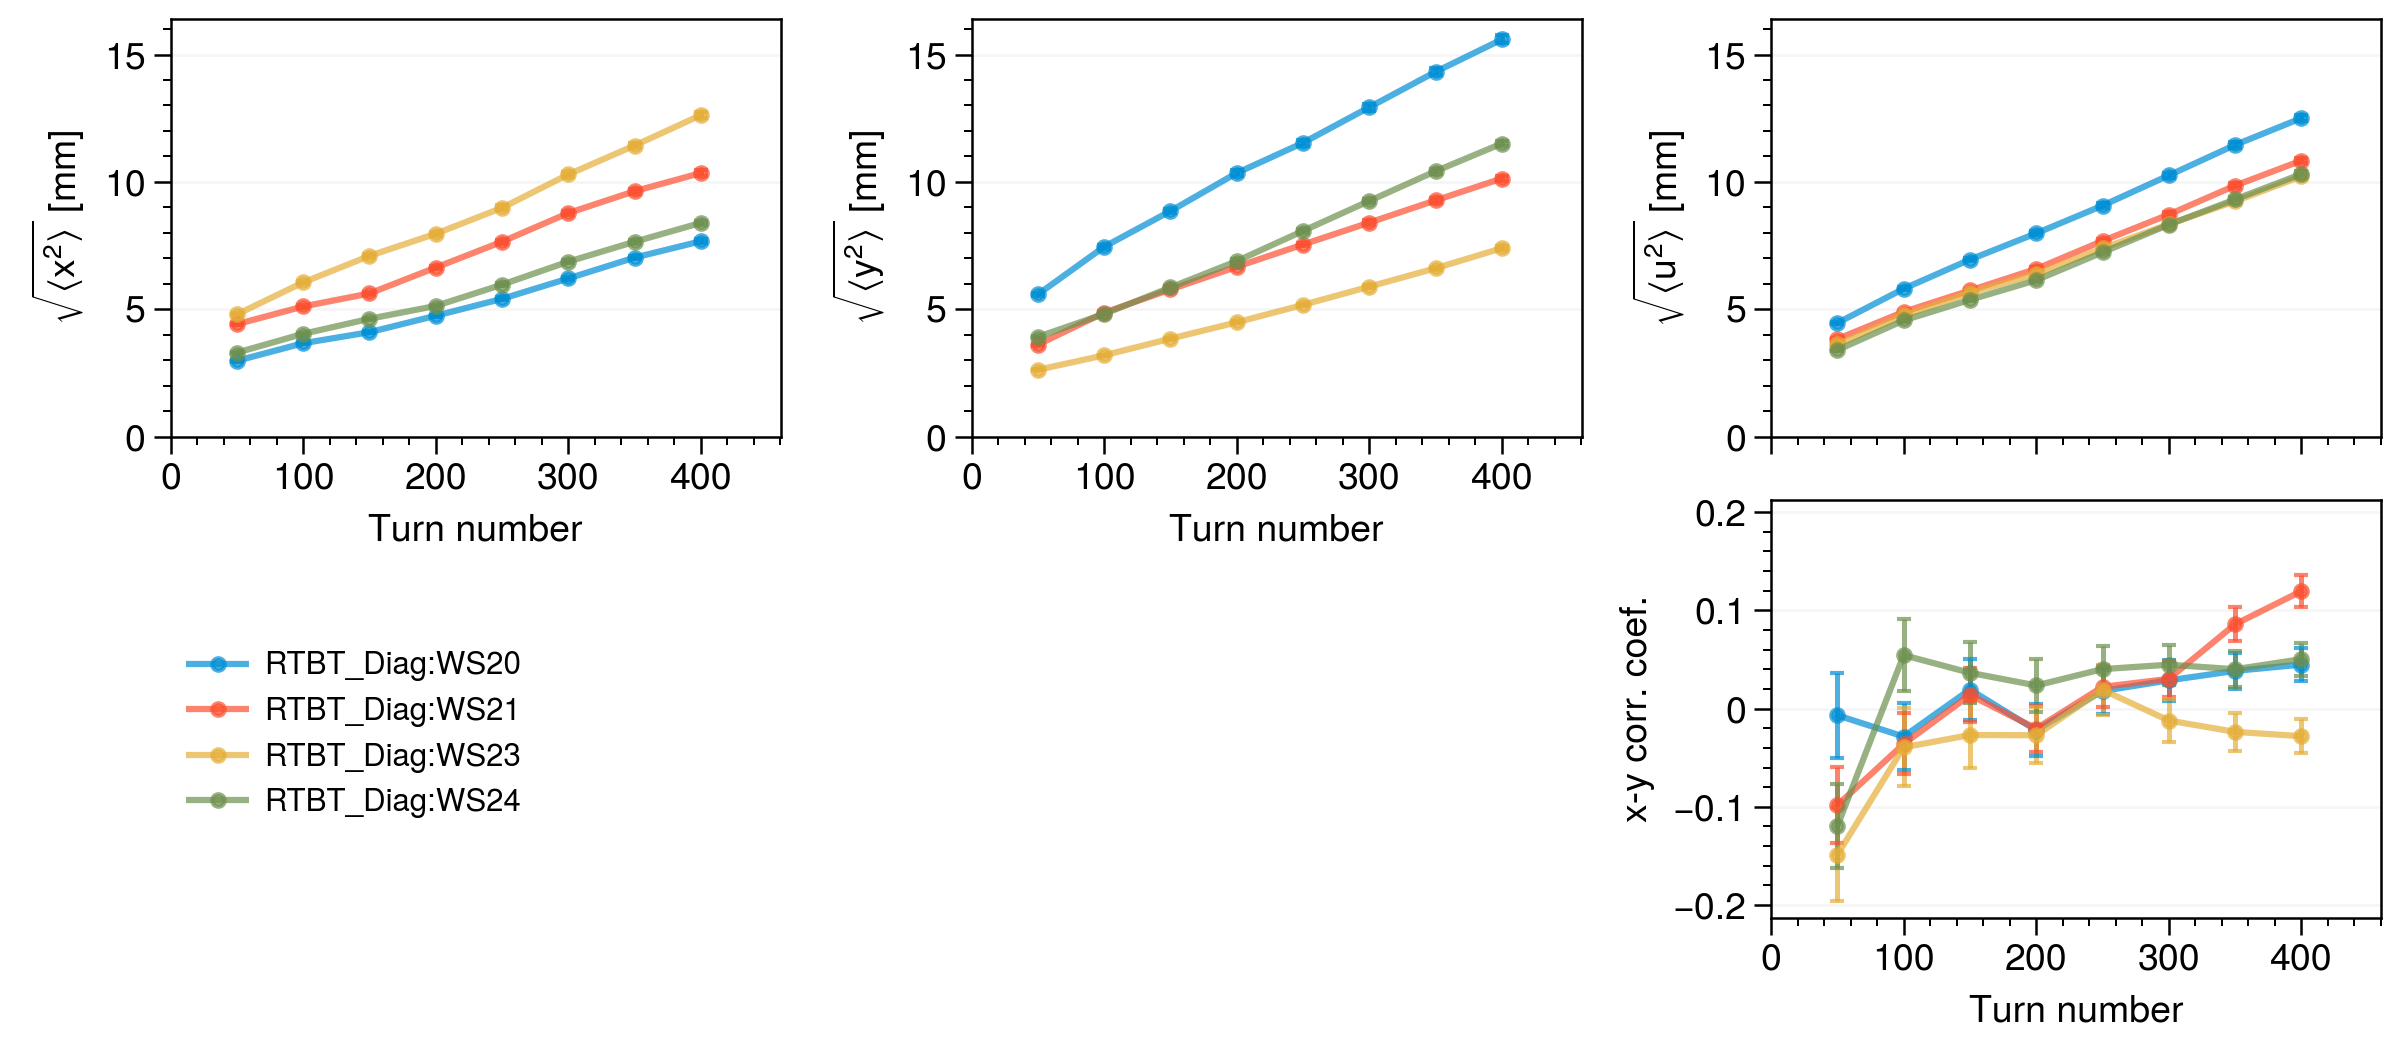
\includegraphics[width=\textwidth]{Images/chapter5/exp3/rms.png}
    \end{subfigure}
    \caption{Measured wire-scanner profiles from Experiment 3.}
    \label{fig:exp3_wsmeas}
\end{figure}
%
%
\begin{figure}[!p]
    \centering
    \begin{subfigure}{0.6\textwidth}
        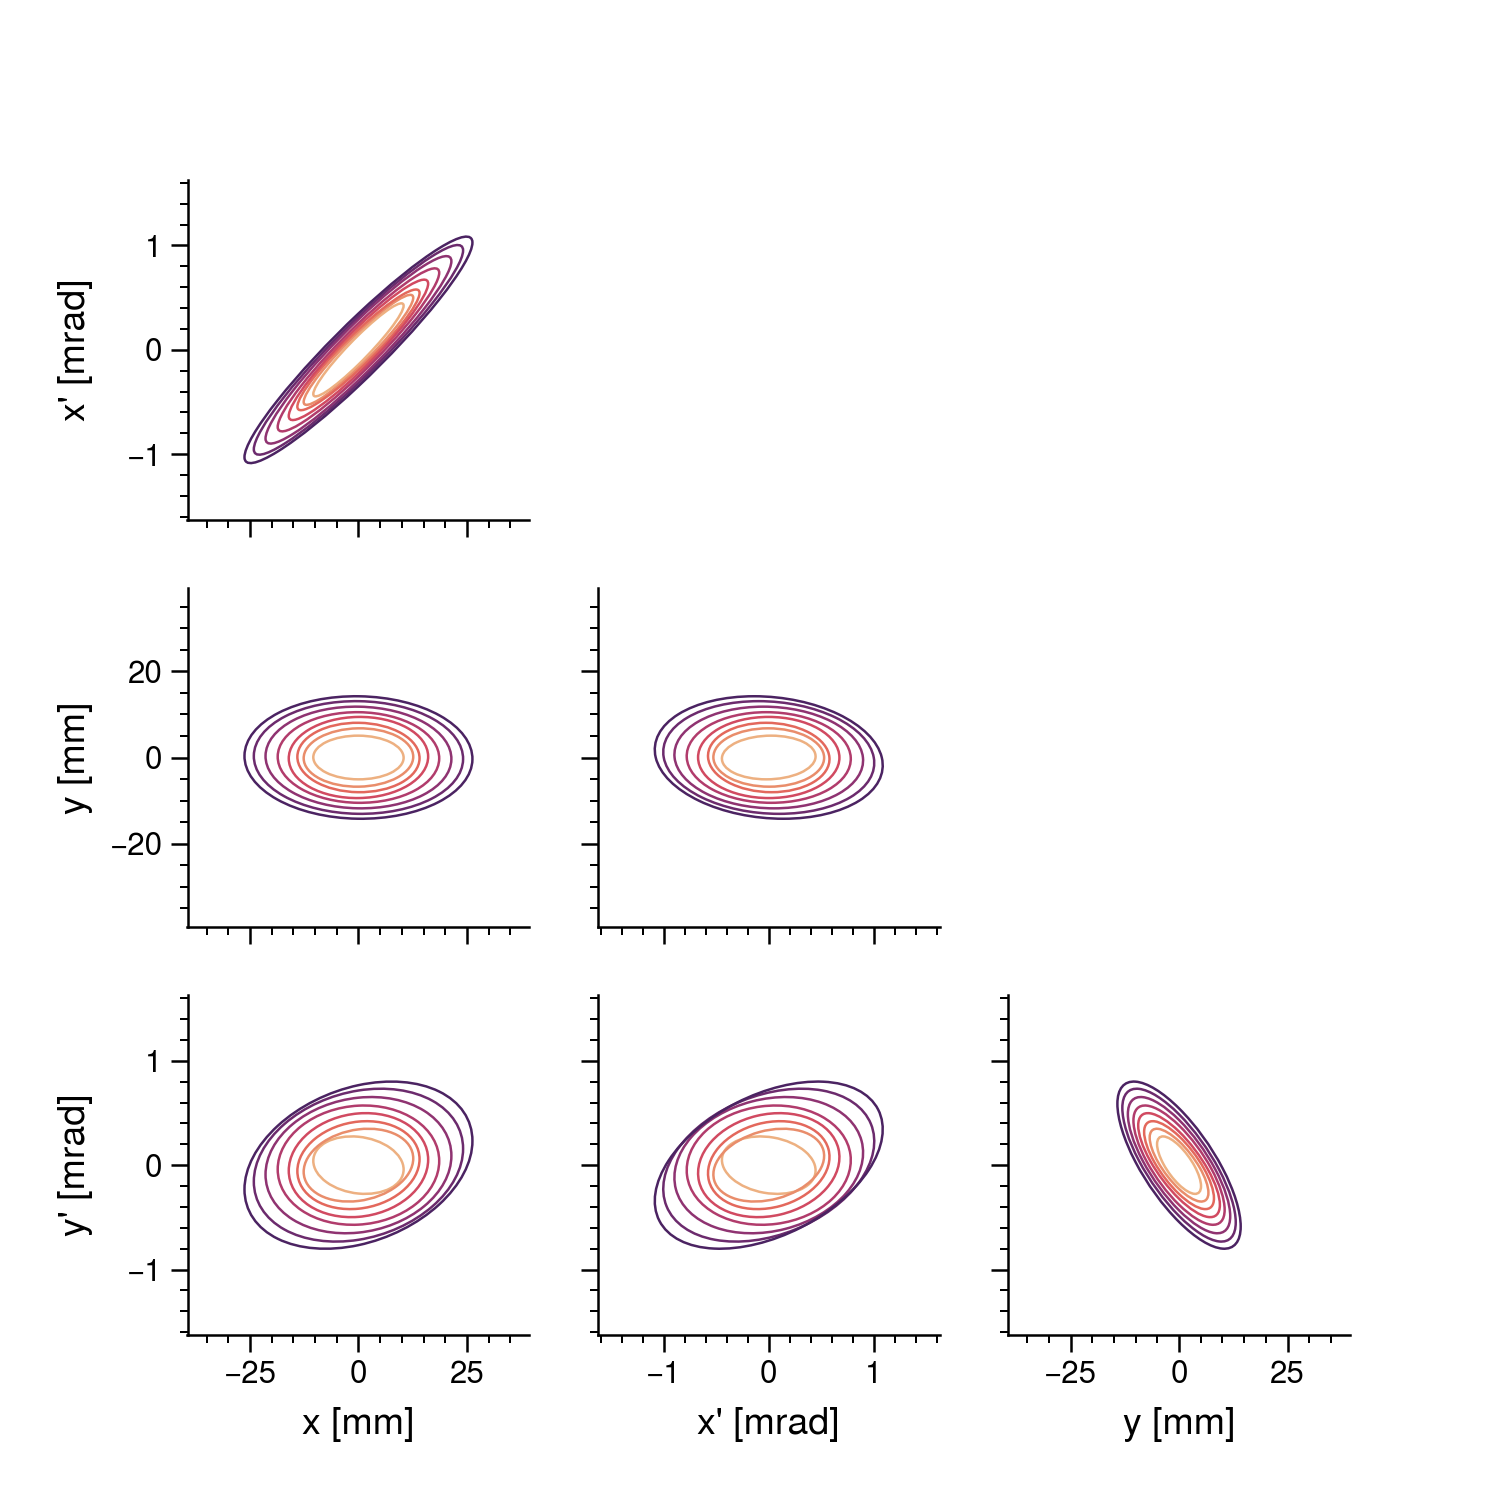
\includegraphics[width=\textwidth]{Images/chapter5/exp3/corner.png}
    \end{subfigure}
    \hfill
    \begin{subfigure}[t]{0.39\textwidth}
        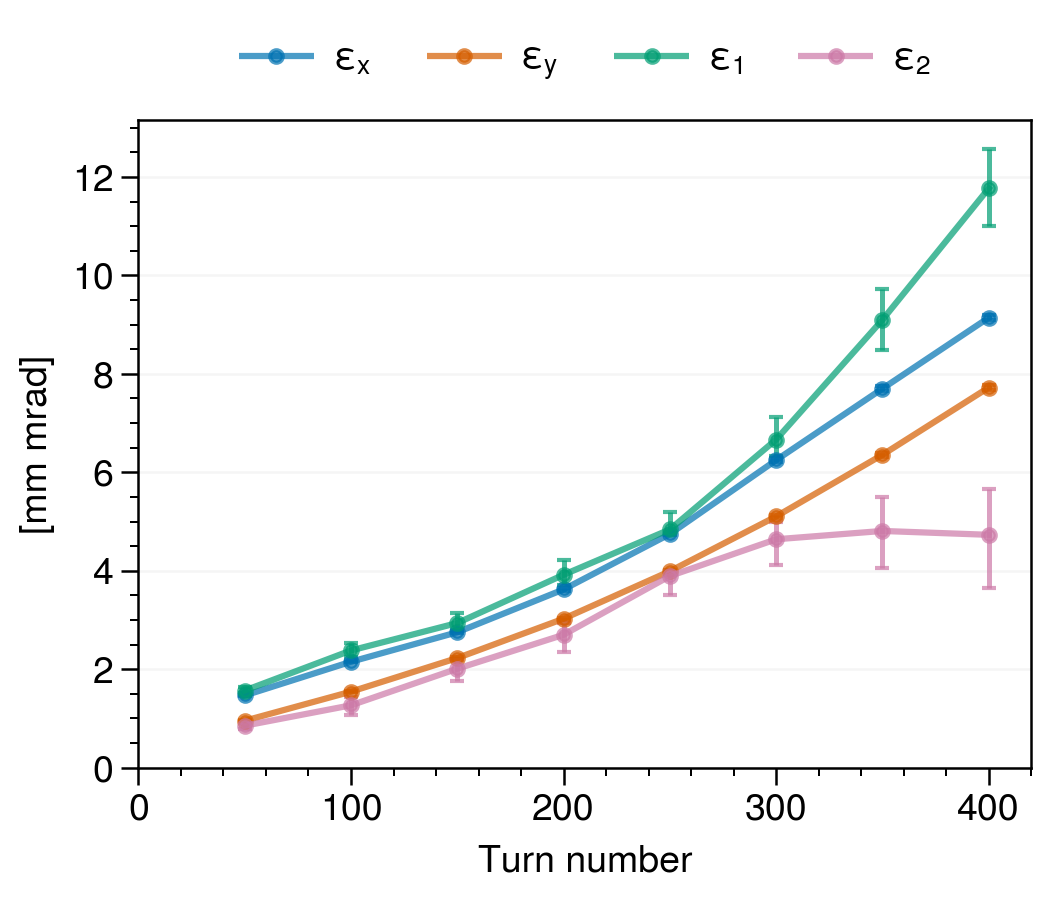
\includegraphics[width=\textwidth]{Images/chapter5/exp3/emittances.png}
    \end{subfigure}
    \caption{Reconstructed emittances and covariance ellipses from Experiment 3.}
    \label{fig:exp3_emittances}
\end{figure}
% 

Notice that $\varepsilon_{1,2}$ significantly deviate from $\varepsilon_{x,y}$ after 300 turns. This was the largest cross-plane correlation measured so far. For additional comparison with the previous experiments, it is helpful to reconstruct the covariance matrix at different locations in the RTBT, which will not change the emittances but will change the correlations between the phase space coordinates. The reconstructed cross-plane correlation coefficients are plotted in Fig.~\ref{fig:exp3_compare_corr} for Experiments 3, 2, and 1a.
%
\begin{figure}[!p]
    \centering
    \vspace*{3.0cm}
    \begin{subfigure}{0.32\textwidth}
        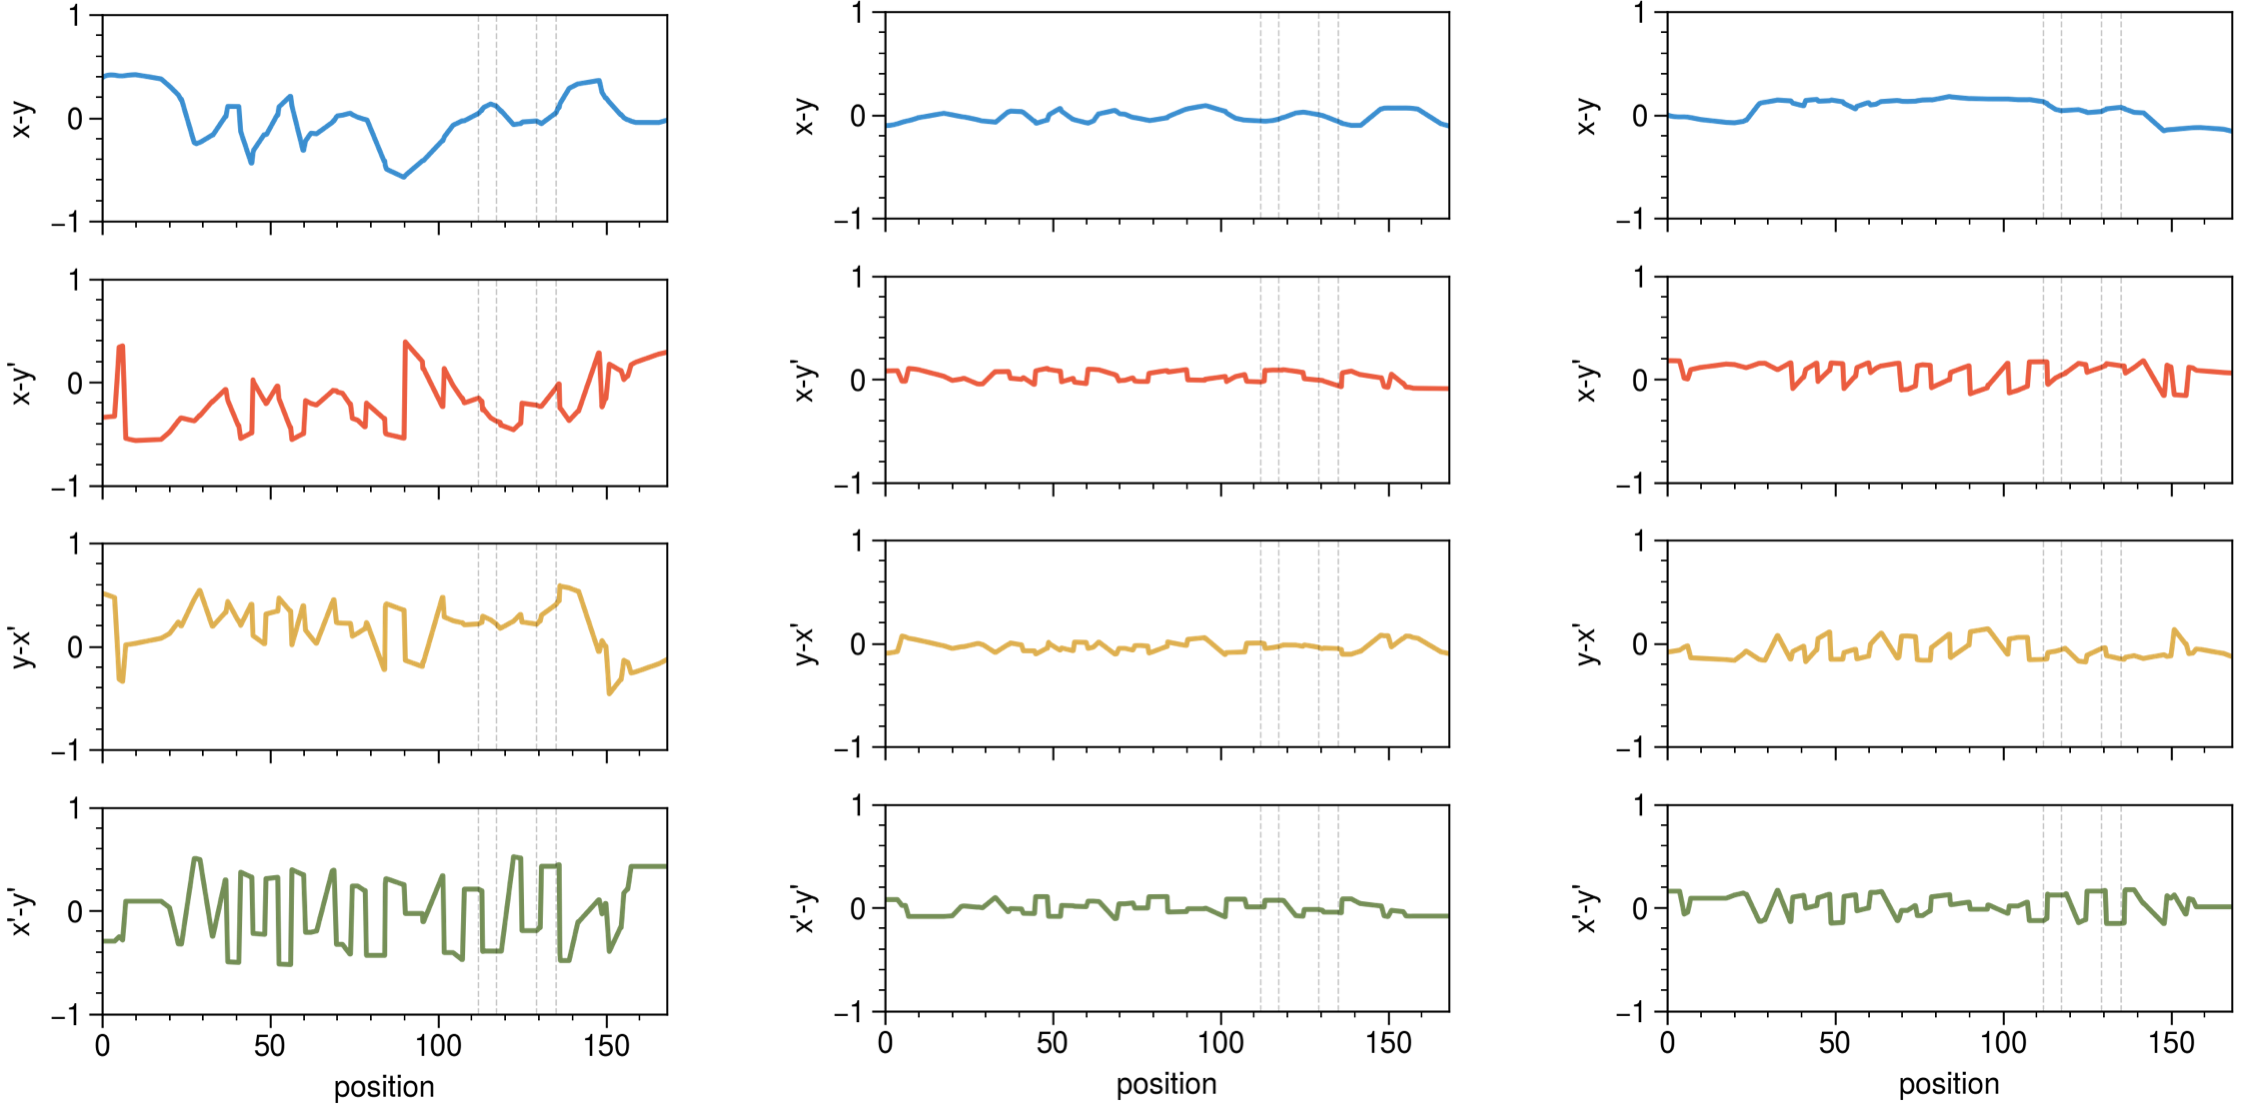
\includegraphics[width=\textwidth]{Images/chapter5/exp3/compare_corr.png}
    \end{subfigure}
    \hfill
    \begin{subfigure}{0.32\textwidth}
        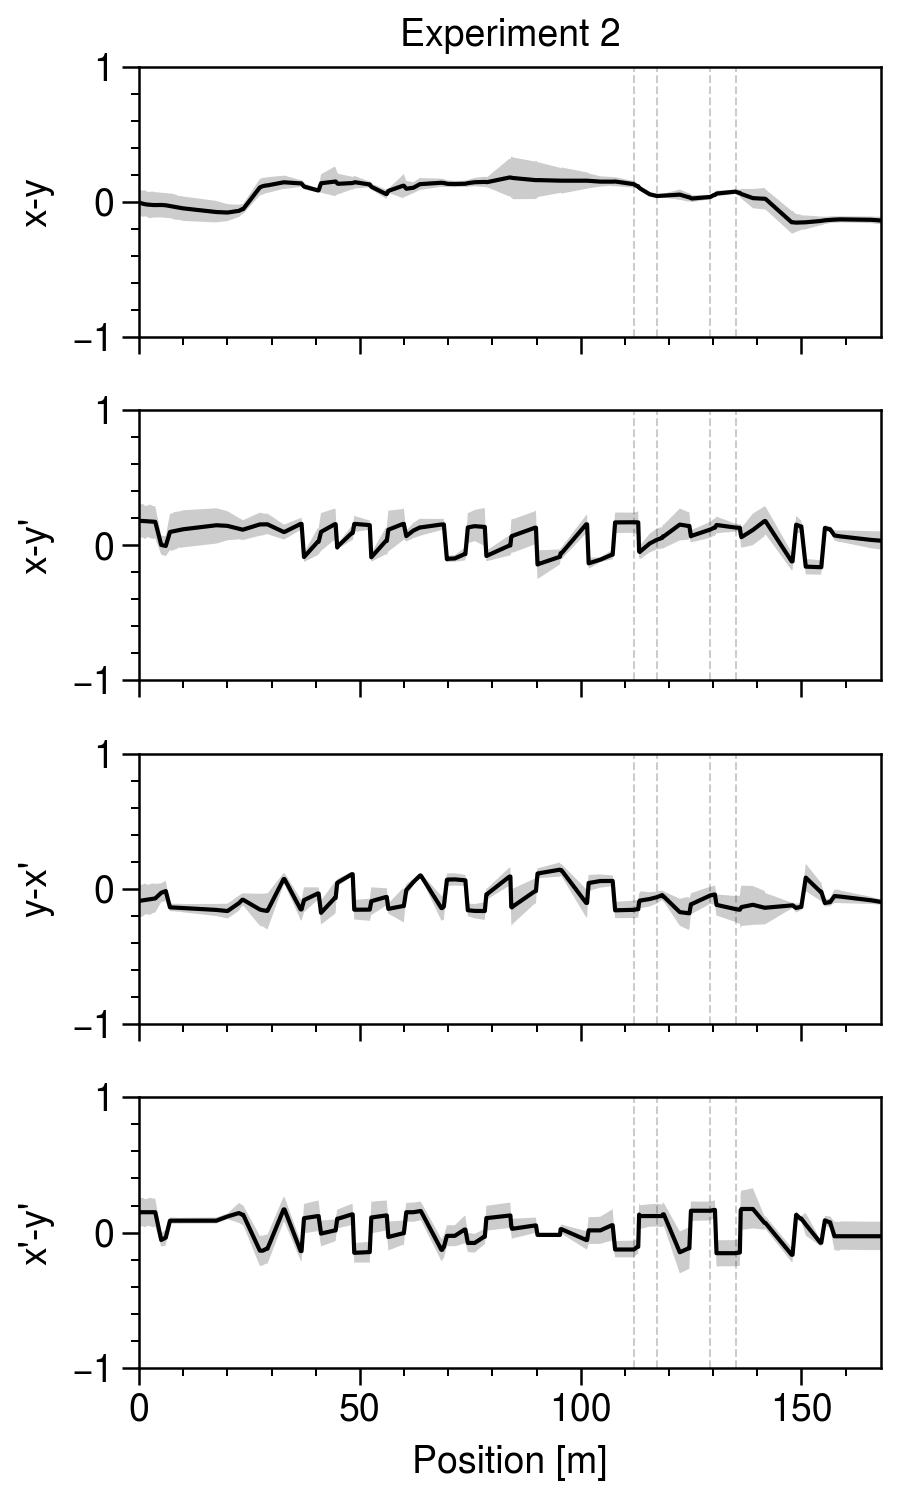
\includegraphics[width=\textwidth]{Images/chapter5/exp2/compare_corr.png}
    \end{subfigure}
    \hfill
    \begin{subfigure}{0.32\textwidth}
        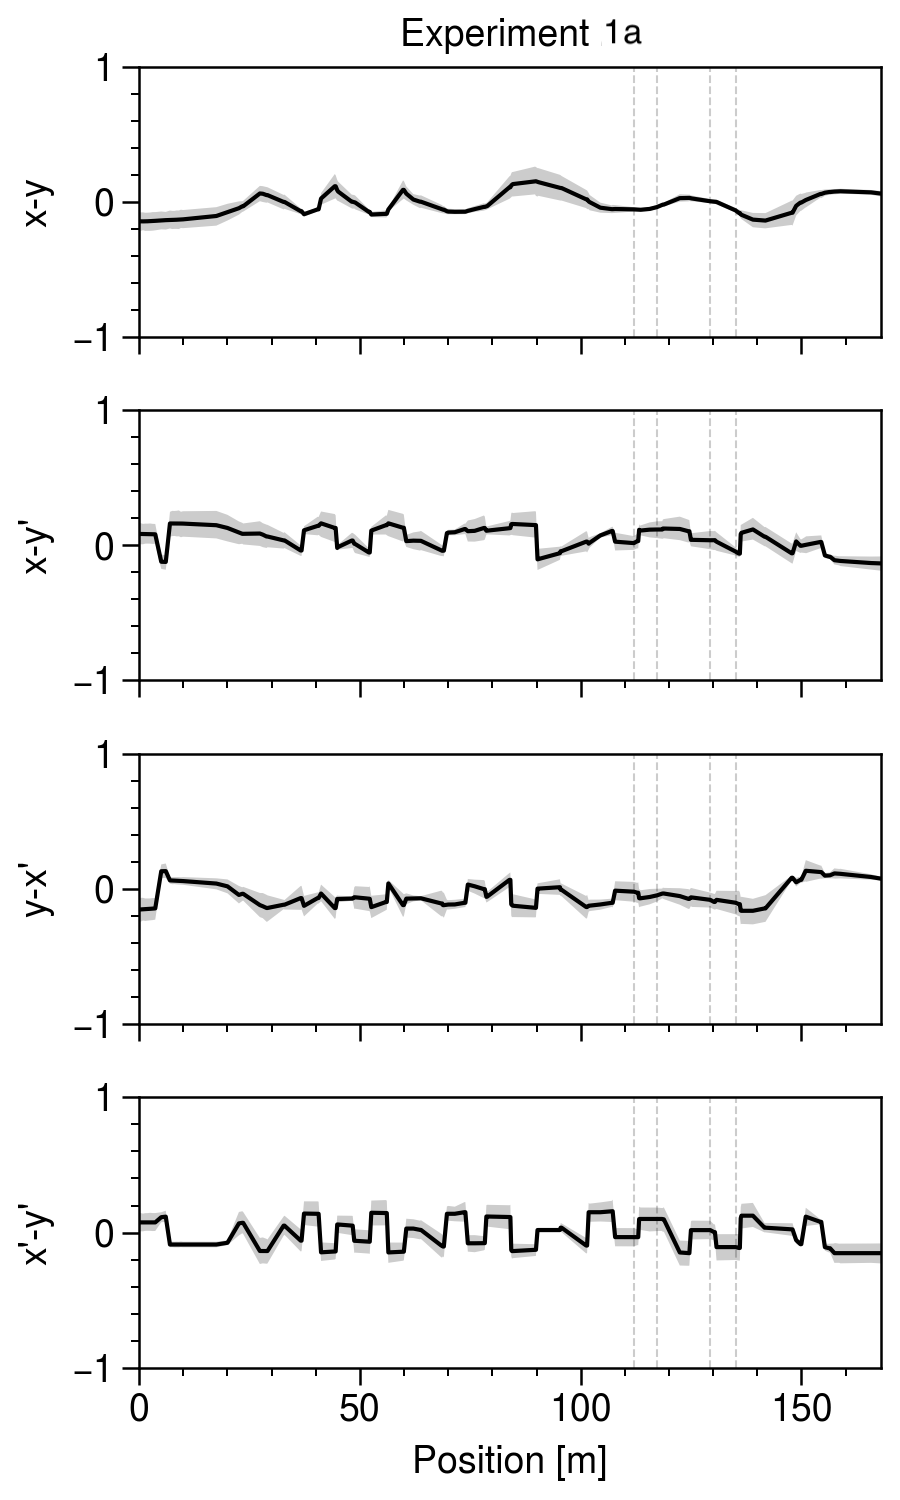
\includegraphics[width=\textwidth]{Images/chapter5/exp1a/compare_corr.png}
    \end{subfigure}
    \caption{Reconstructed cross-plane correlation coefficients for Experiments 3, 2, and 1a.}
    \label{fig:exp3_compare_corr}
    \vspace*{3.0cm}
\end{figure}
% 
The black lines represent the reconstructed values, and the grey regions represent the standard deviation across the random trials with noise added to the measured moments. In a beam with a reduced 4D emittance, these coefficients should exhibit a strong dependence on the external focusing; hence, Fig.~\ref{fig:exp3_compare_corr} is evidence that the painting method has produced a beam with reduced 4D emittance.

At the end of this experiment, beam images on the target were collected as the horizontal and vertical phase advances were scanned. The initial script used $15 \times 15$ phase advances, storing all the images in one array, but this caused the program to crash on step 150 due to a memory error. At this point there was not much time remaining in the control room, so a second script was run that used $7 \times 7$ phase advances. Unfortunately, it was overlooked that the optics in the RTBT had already been modified for the wire-scanner measurements; the required magnet changes were eventually too large and it was decided to stop the program after 43/49 images had been collected. Additional problems include that the pause between changing the optics, triggering the beam, and collecting the images was apparently not long enough, so there were several blanks and duplicates in the image set, and that the beam length was inadvertently changed from 45/64 to 15/64 of the ring length, so the distribution was not the same as in the wire-scanner measurement. For this last reason, we cannot directly compare with the wire-scanner measurement. Nonetheless, two of the images are shown in Fig.~\ref{fig:exp3_target_scan}. 
%
\begin{figure}[!p]
    \centering
    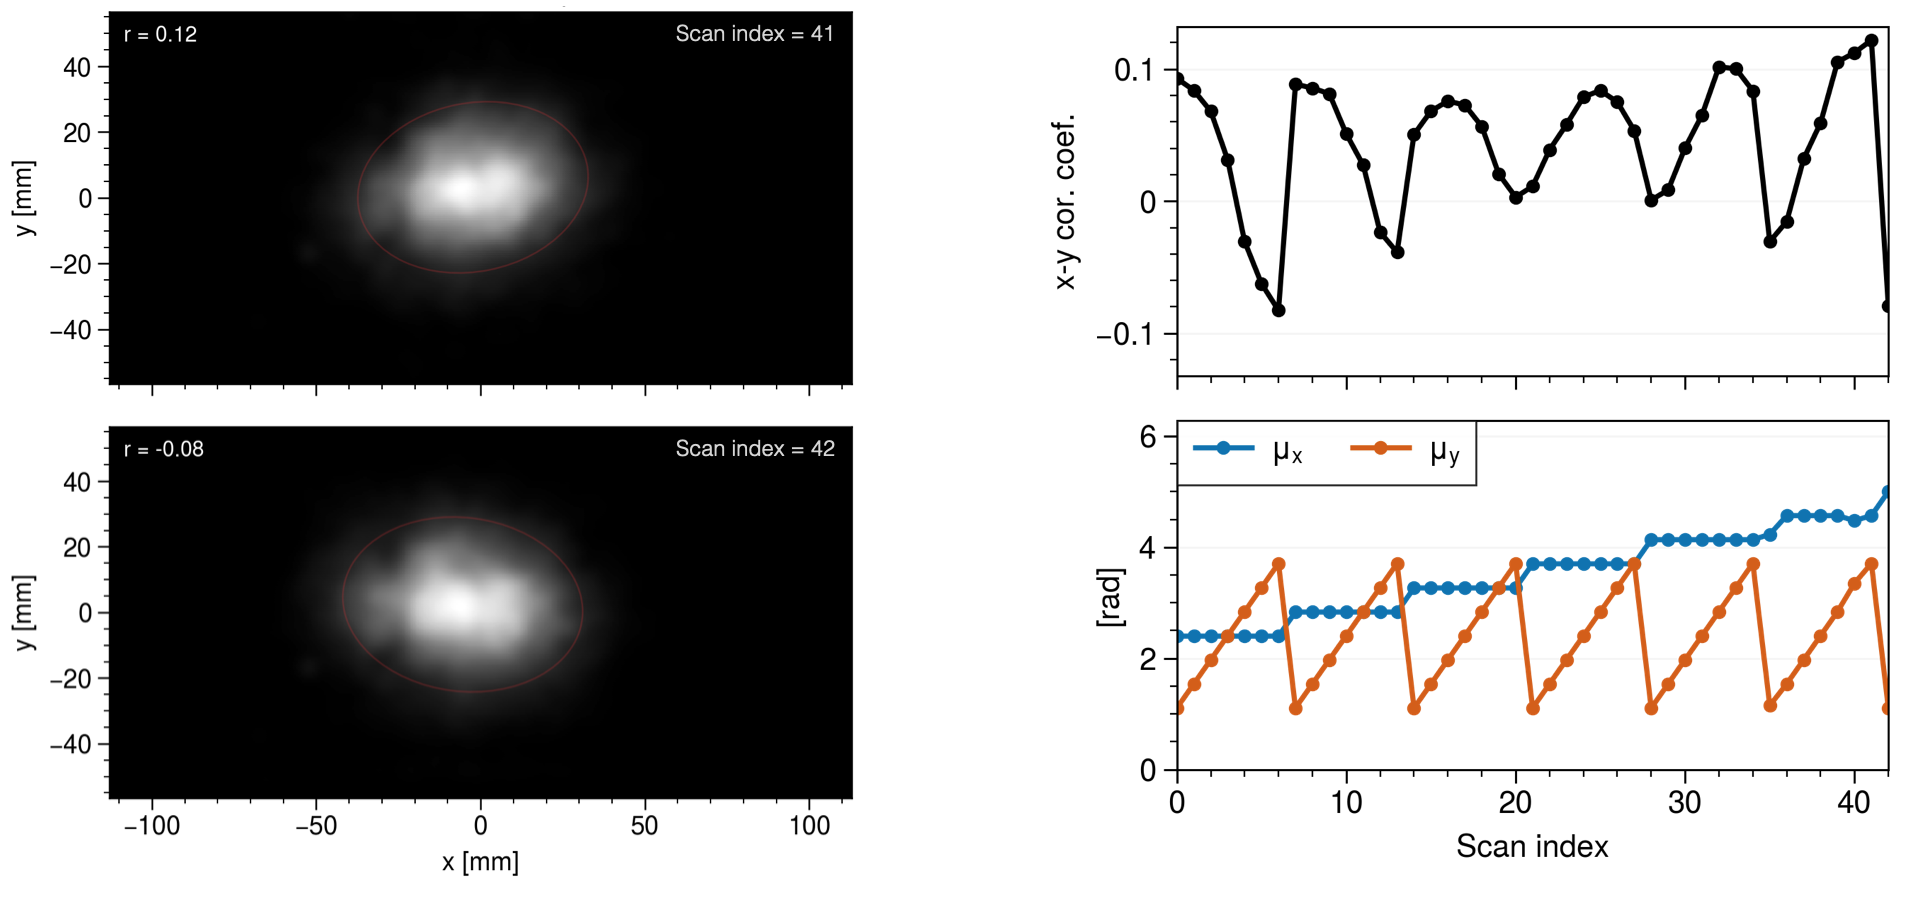
\includegraphics[width=\textwidth]{Images/chapter5/exp3/target_scan/target_scan.png}
    \caption{Scan of the phase advances at the target. Left: processed images on last two steps in the scan. Top right: $x$-$y$ correlation coefficients computed from the images. Bottom right: Phase advances at the target.}
    \label{fig:exp3_target_scan}
\end{figure}
%
The $x$-$y$ correlation coefficient\footnote{The $x$-$y$ correlation coefficient is calculated directly from the image.}, although small, clearly depends on the phase advances, demonstrating that there is cross-plane correlation in the beam. It is therefore recommended to repeat this measurement for comparison with the wire-scanner reconstruction. We also note that if a beam with small 4D emittance is produced in the future, arranging the target images in matrix form as in Fig.~\ref{fig:tomo_sim_target_scan} could be useful even without applying a reconstruction algorithm to the images. 

We conclude with a simulation of this experiment in Fig.~\ref{fig:exp3_sim}.
%
\begin{figure}[!p]
    \centering
    \begin{subfigure}{0.85\textwidth}
        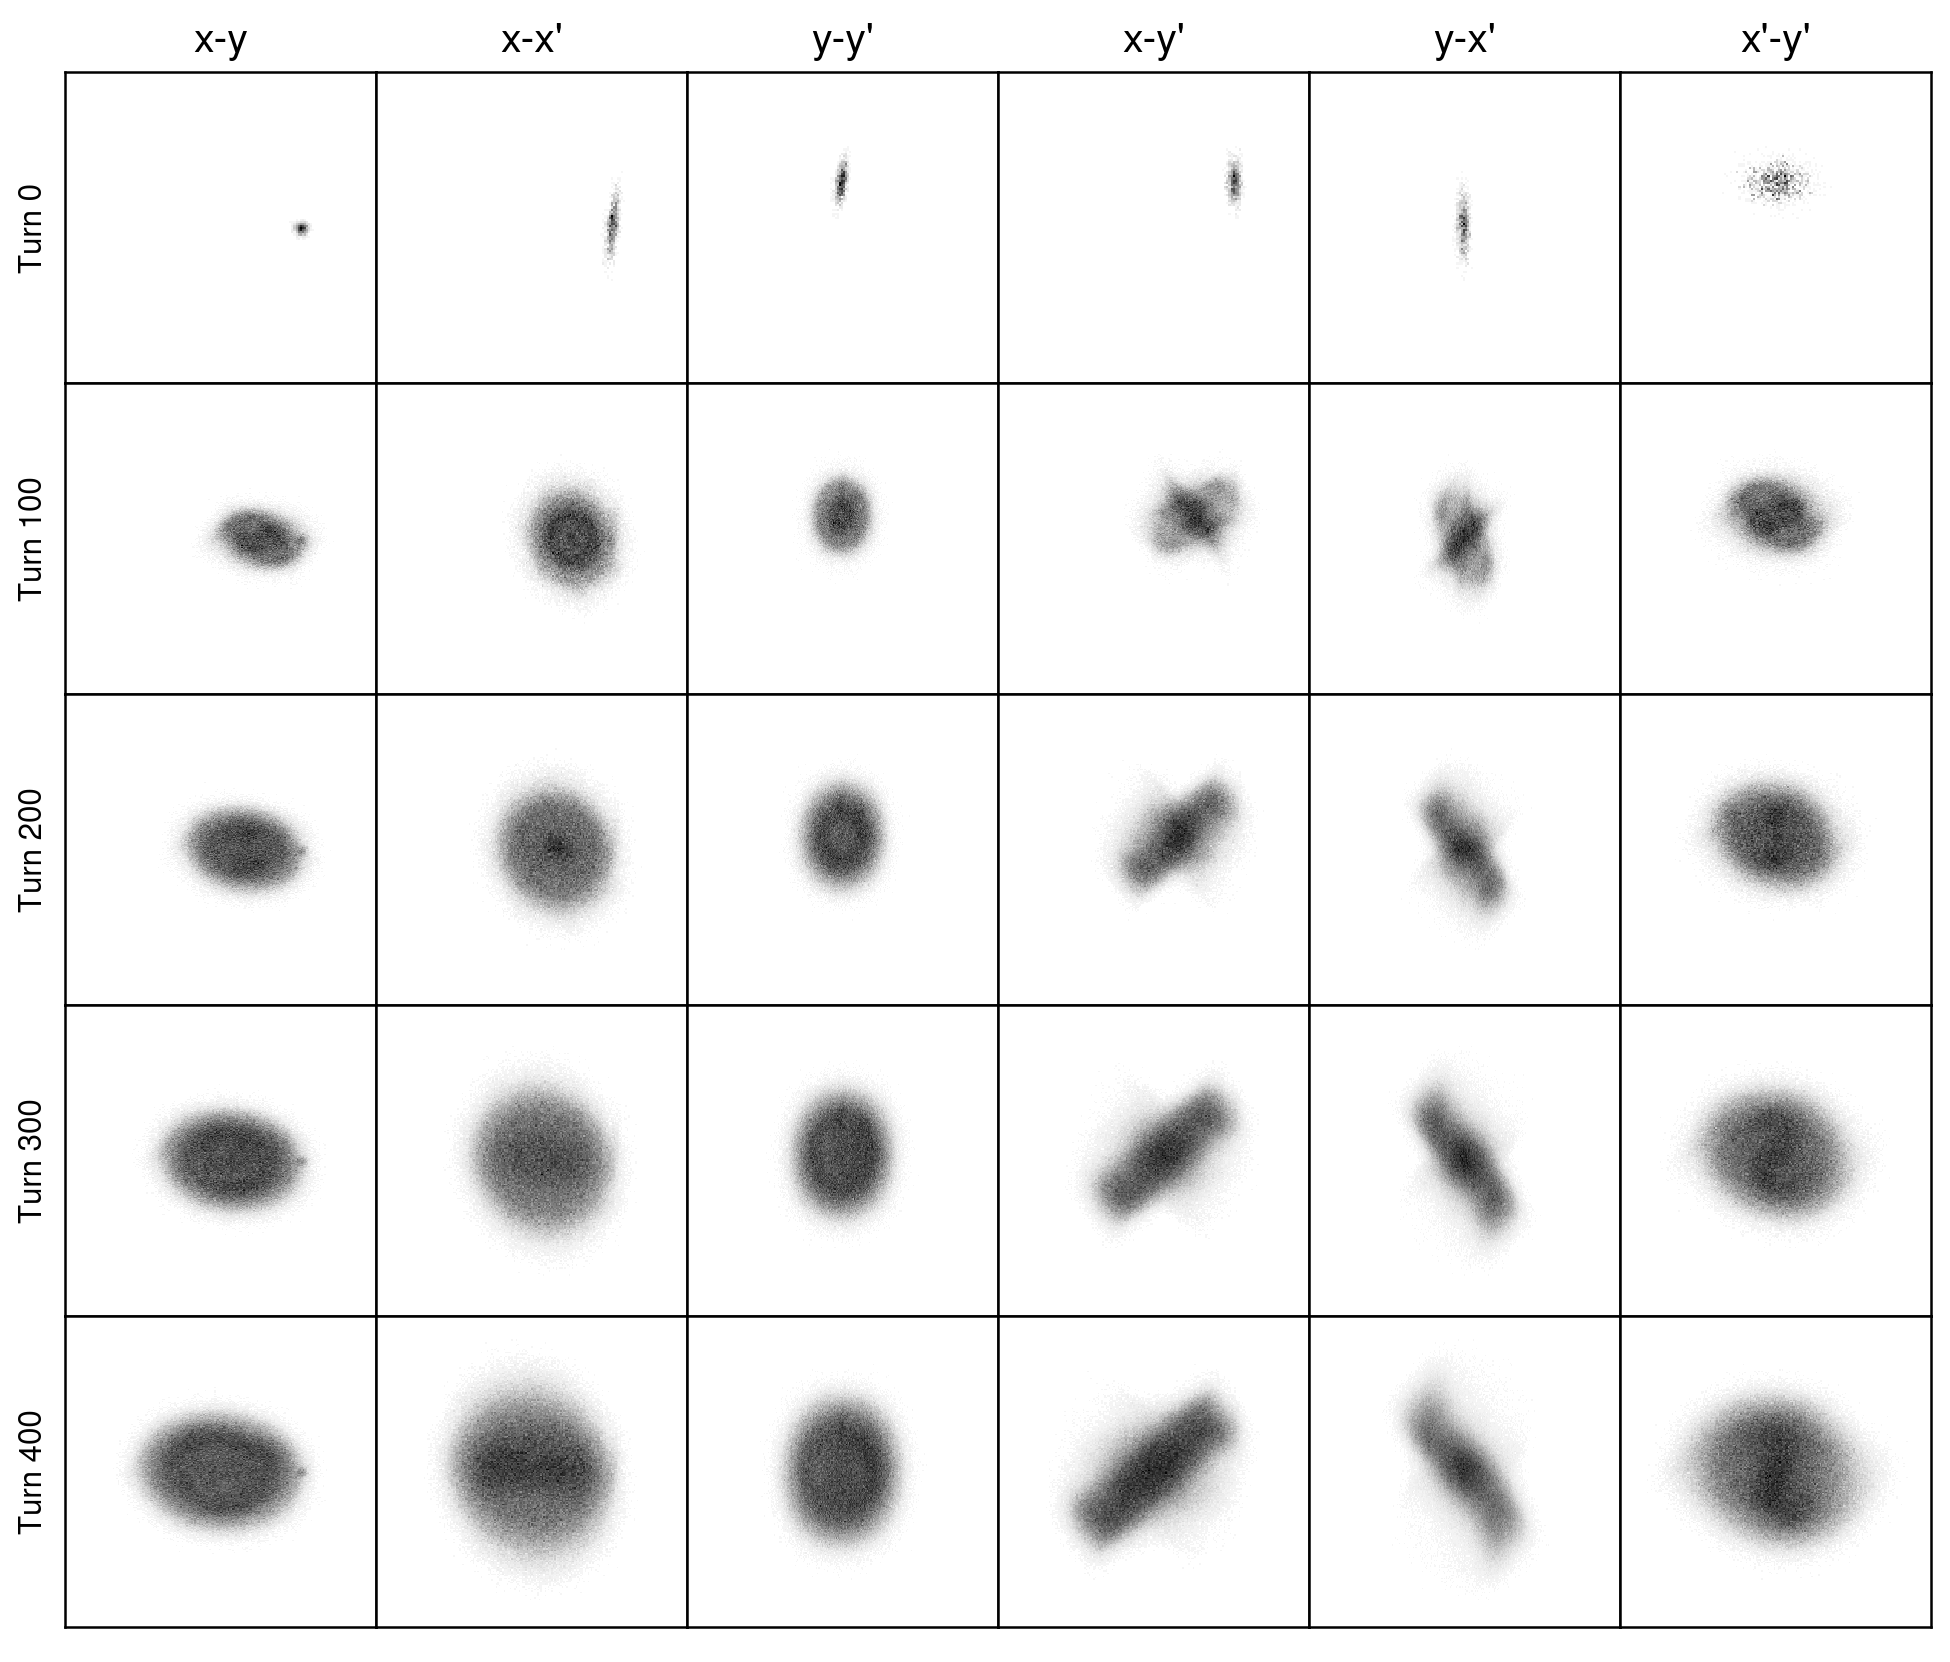
\includegraphics[width=\textwidth]{Images/chapter5/exp3/sim_snapshots.png}
    \end{subfigure}
    \vfill
    \vspace*{1.0cm}
    \vfill
    \begin{subfigure}{0.7\textwidth}
        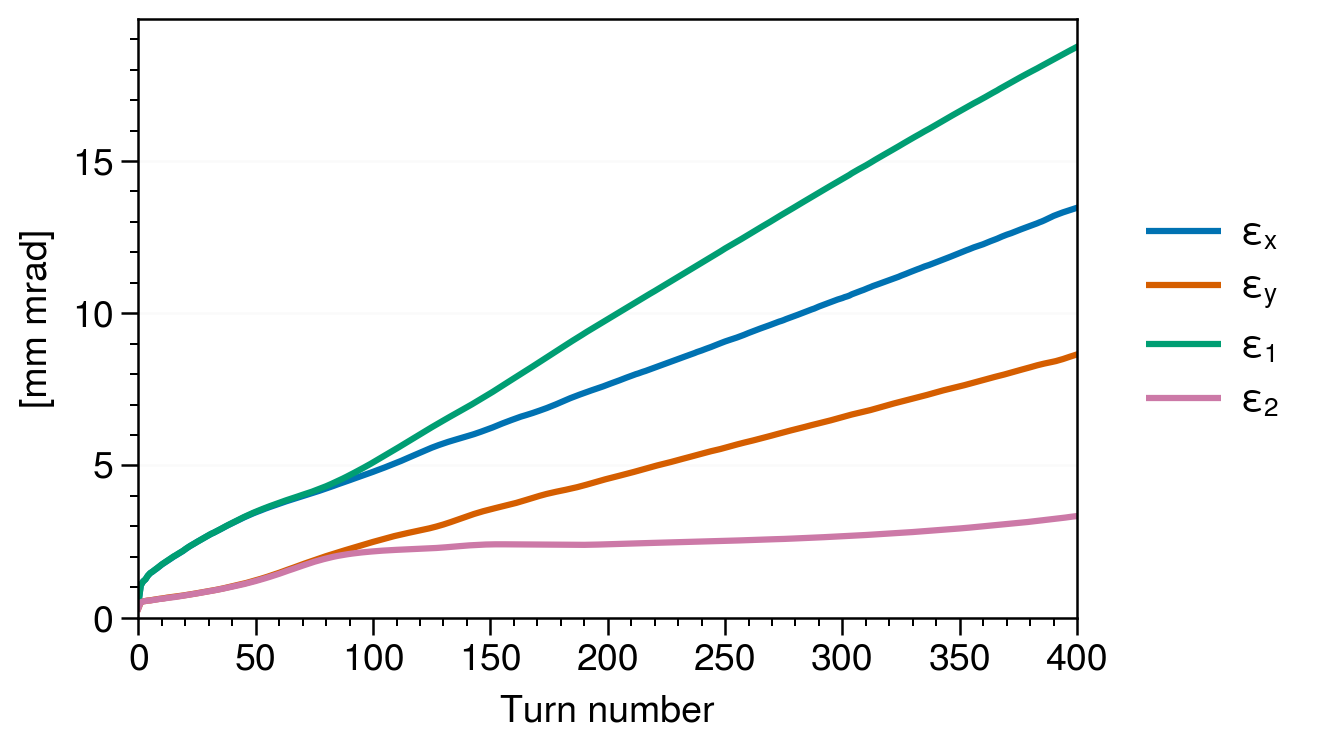
\includegraphics[width=\textwidth]{Images/chapter5/exp3/sim_emittances.png}
    \end{subfigure}
    \caption{Simulation of Experiment 3.}
    \label{fig:exp3_sim}
\end{figure}
%
This looks closer to the best-case scenario from Chapter \ref{chap-3}, even through solenoids are not present in the ring and the vertical slope from the kickers is limited. Again, the predicted ratio $\varepsilon_1 / \varepsilon_2$ is larger than what was measured; however, the simulations of Experiment 2/3 differ in a similar way to the measurements of Experiment 2/3. Namely, in Experiment 3, the smaller intrinsic emittance curve flattens as injection progresses and the final ratio $\varepsilon_1 / \varepsilon_2$ is larger than in Experiment 2. 

We note that the zero-current tunes in the simulation were equal at $\nu_x = \nu_y = 6.18$. The measured tunes were also equal, but there may be some uncertainty in the measurement; therefore, simulation was repeated as the horizontal tune was varied in steps of 0.005. At $\nu_x = 6.19$, there was not a large change from the original case. At $\nu_x = 6.2$, the cross-plane correlation in the beam was eliminated. Fig.~\ref{fig:exp3_sim_nux6.195_nuy6.18} shows the case when $\nu_x = 6.195$. 
%
\begin{figure}[!p]
    \centering
    \begin{subfigure}{0.85\textwidth}
        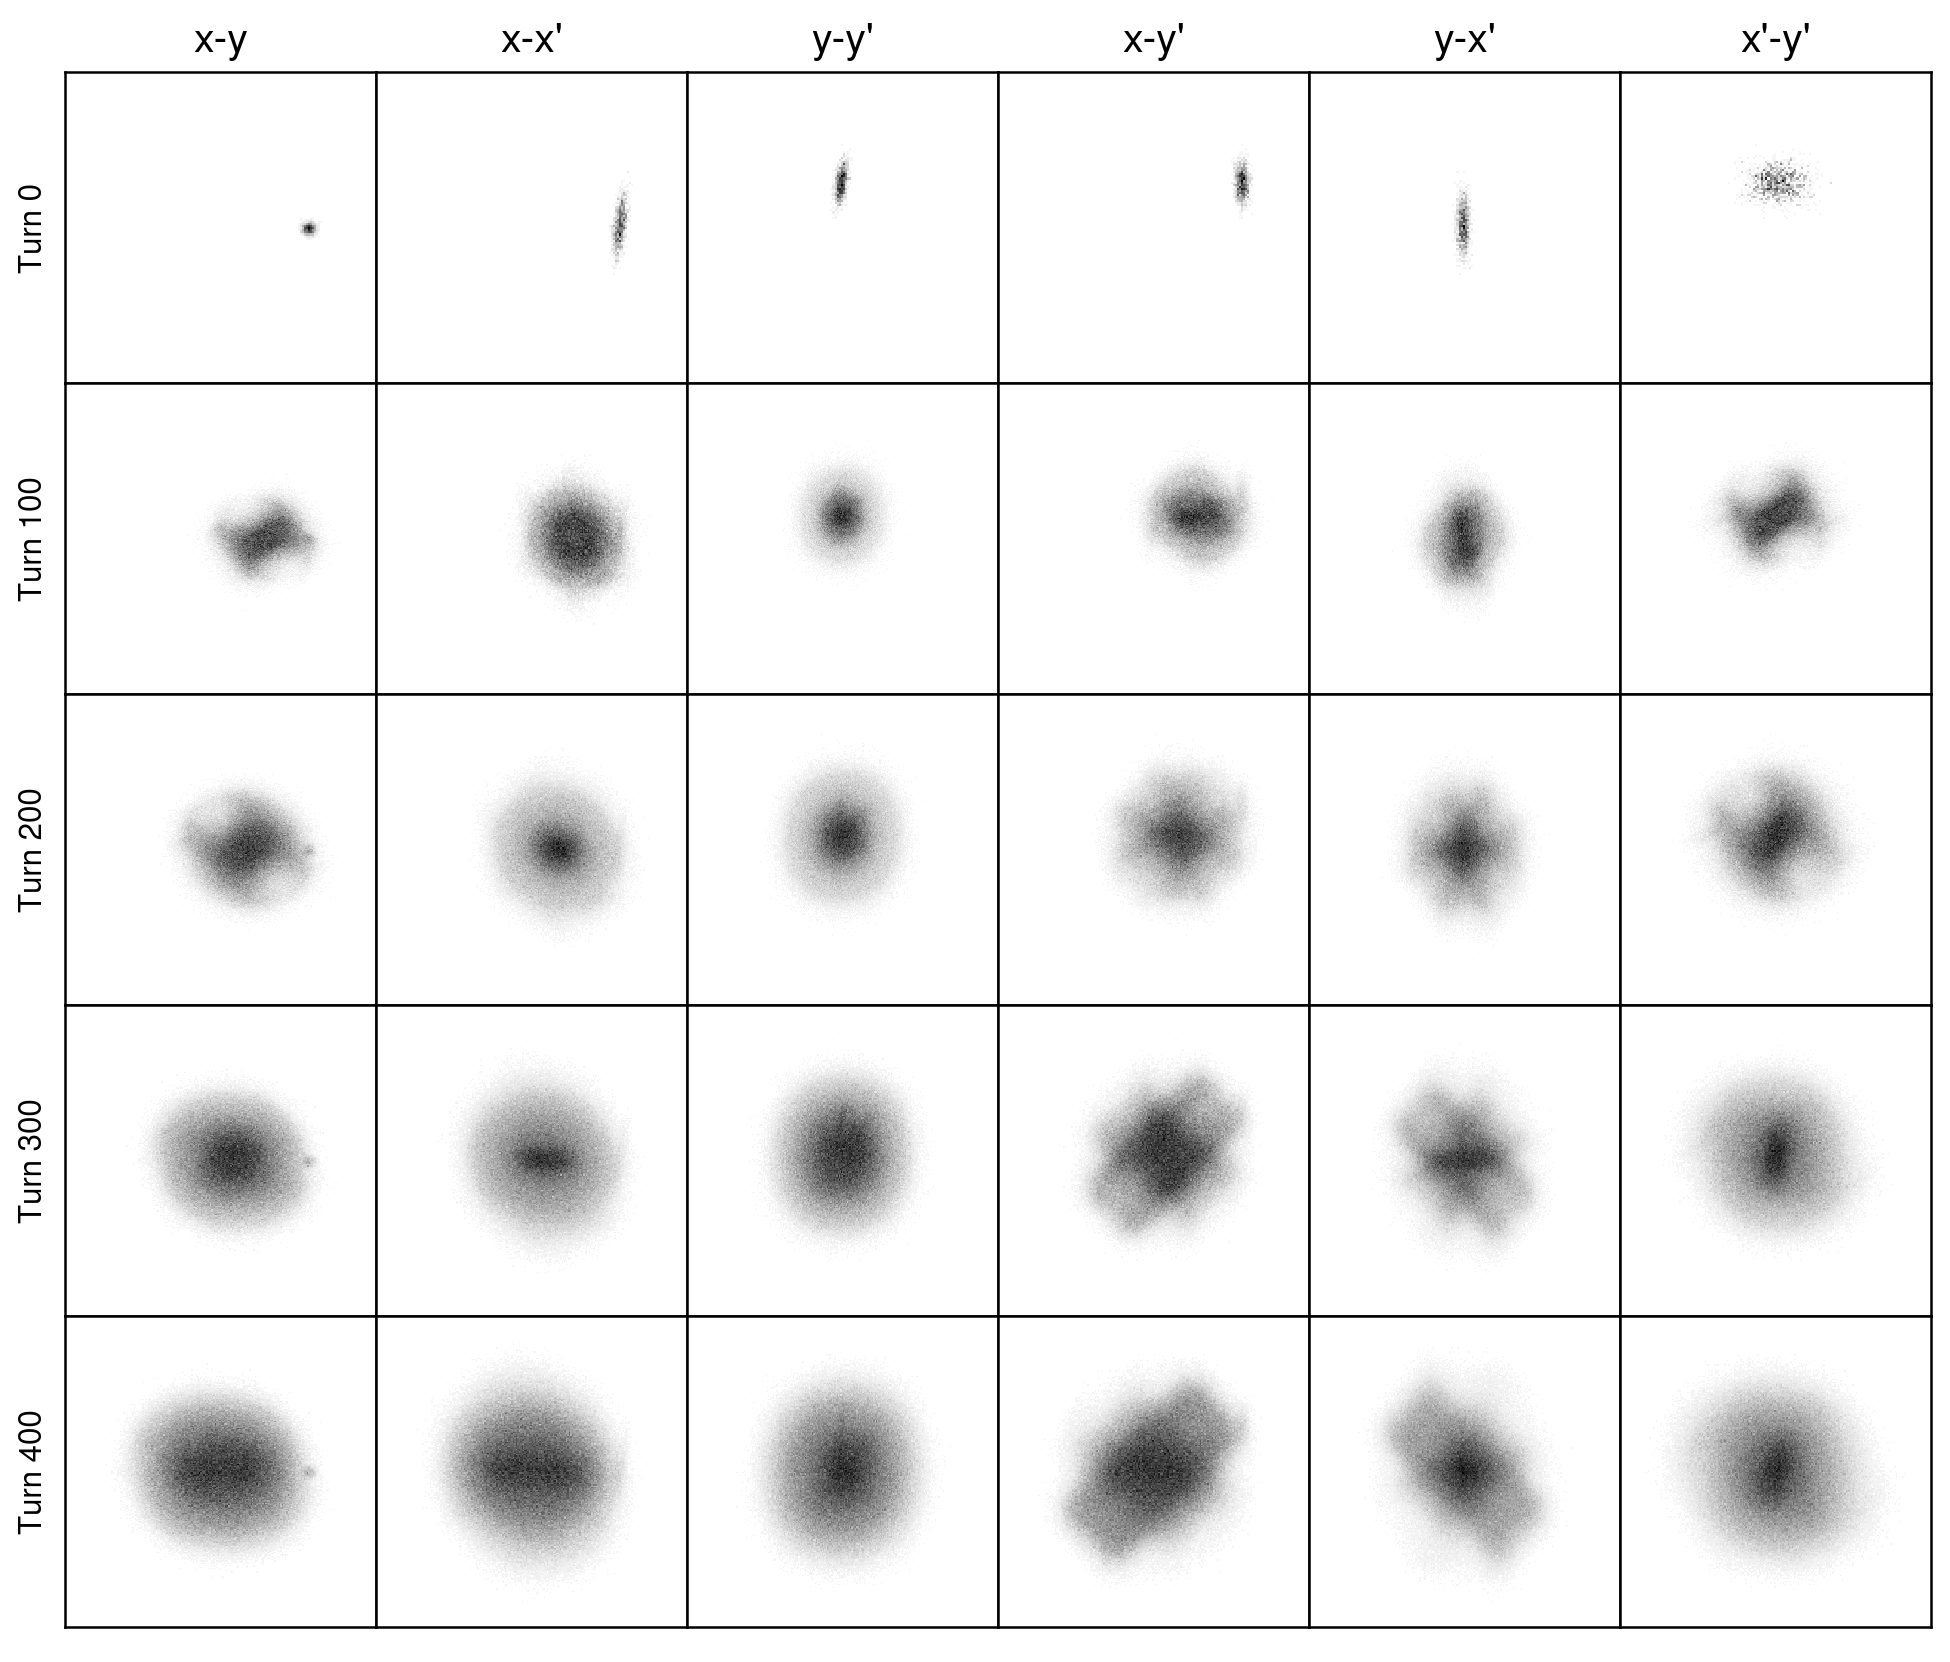
\includegraphics[width=\textwidth]{Images/chapter5/exp3/sim_snapshots_nux6.195_nuy6.18.png}
    \end{subfigure}
    \vfill
    \vspace*{1.0cm}
    \vfill
    \begin{subfigure}{0.7\textwidth}
        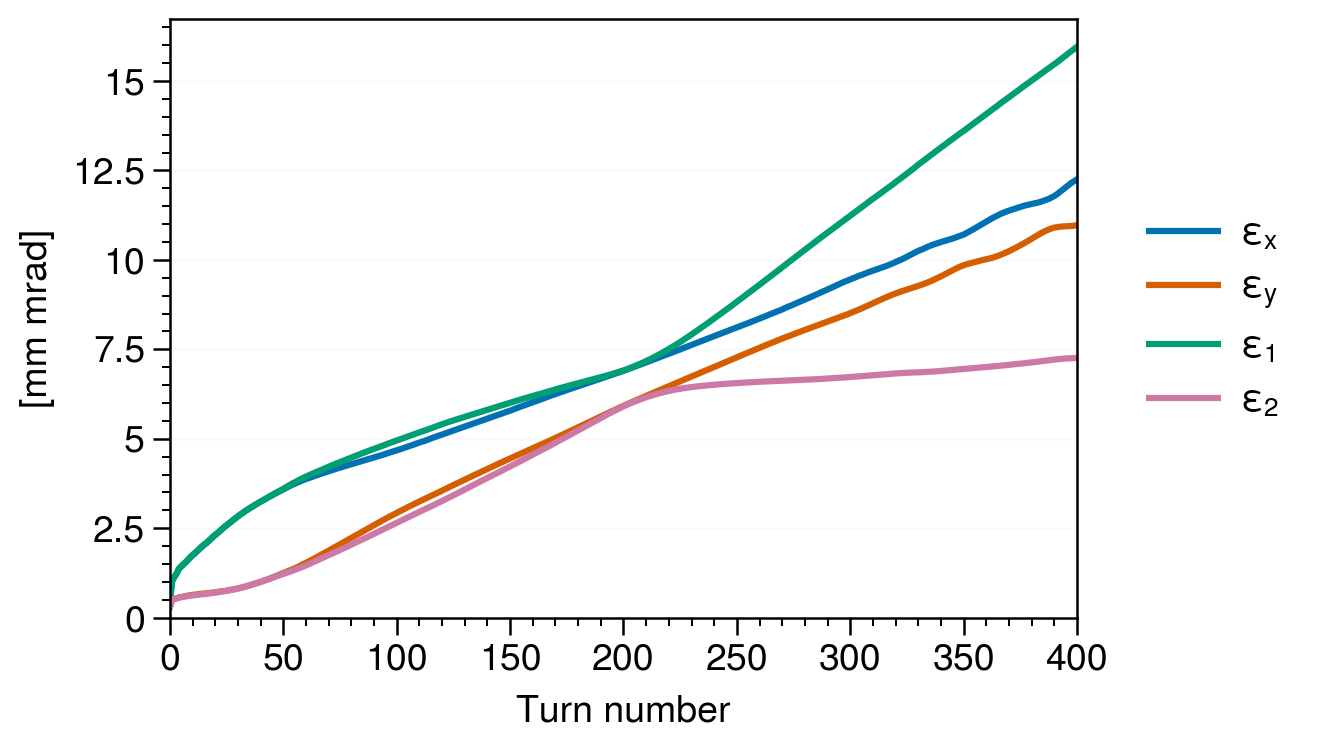
\includegraphics[width=\textwidth]{Images/chapter5/exp3/sim_emittances_nux6.195_nuy6.18.png}
    \end{subfigure}
    \caption{Simulation of Experiment 3 with $\nu_x = 6.195$, $\nu_y = 6.18$.}
    \label{fig:exp3_sim_nux6.195_nuy6.18}
\end{figure}
%
The time at which the intrinsic emittances diverge from the apparent emittances has been pushed later in injection, more closely resembling the measurements in Fig.~\ref{fig:exp3_emittances}. We thus accept the hypothesis that this simulation is an accurate representation of reality. If this is hypothesis is valid, it raises the probability that the simulated `best-case scenario" in Chapter \ref{chap-3} can be approached future with further tuning of the ring and with the addition of solenoid magnetic fields.




\section{Experiment 4}

[Jan. 2022]


\section{Summary}

The goal of the experiments in this chapter was to carry out elliptical painting in the SNS and measure the painted distribution. This has been accomplished. In Experiment 1, the Ring Injection Control (RIC) application was tested at 1 GeV beam energy and a procedure to efficiently measure the emittance during injection was identified. It was also found that lowering the beam energy was necessary to move the closed orbit to the foil. In Experiment 2, the beam energy was lowered to 0.8 GeV. Measurements showed that particles were injected near the closed orbit at the start of injection, and that the beam size grew with approximate square root time-dependence. A small split in the intrinsic emittances was measured near the end of injection. Simulations indicated that increasing the beam size and reducing the beam intensity would have a positive effect. In Experiment 3, the beam length, transverse size, and intensity were varied. The most promising case — 20\% reduction in beam intensity and 150\% increase in horizontal beam size — was investigated in more detail. A larger split in the intrinsic emittances was measured near the end of injection. Additionally, the tilt angle of the beam image on the target was shown to depend on the phase advances at the target. In Experiment 4, [...]. These results are promising: variation of the machine parameters has a significant effect on the painted distribution.